%-------------------------------------------------------------------------------
% This file provides a skeleton ATLAS paper.
%-------------------------------------------------------------------------------
% \pdfoutput=1
% The \pdfoutput command is needed by arXiv/JHEP/JINST to ensure use of pdflatex.
% It should be included in the first 5 lines of the file.
% \pdfinclusioncopyfonts=1
% This command may be needed in order to get \ell in PDF plots to appear. Found in
% https://tex.stackexchange.com/questions/322010/pdflatex-glyph-undefined-symbols-disappear-from-included-pdf
%-------------------------------------------------------------------------------
% Specify where ATLAS LaTeX style files can be found.
\newcommand*{\ATLASLATEXPATH}{latex/}
% Use this variant if the files are in a central location, e.g. $HOME/texmf.
% \newcommand*{\ATLASLATEXPATH}{}
%-------------------------------------------------------------------------------
\documentclass[PAPER, atlasdraft=true, texlive=2016, UKenglish,coverpage]{\ATLASLATEXPATH atlasdoc}
% The language of the document must be set: usually UKenglish or USenglish.
% british and american also work!
% Commonly used options:
%  atlasdraft=true|false This document is an ATLAS draft.
%  texlive=YYYY          Specify TeX Live version (2016 is default).
%  coverpage             Create ATLAS draft cover page for collaboration circulation.
%                        See atlas-draft-cover.tex for a list of variables that should be defined.
%  cernpreprint          Create front page for a CERN preprint.
%                        See atlas-preprint-cover.tex for a list of variables that should be defined.
%  NOTE                  The document is an ATLAS note (draft).
%  PAPER                 The document is an ATLAS paper (draft).
%  CONF                  The document is a CONF note (draft).
%  PUB                   The document is a PUB note (draft).
%  BOOK                  The document is of book form, like an LOI or TDR (draft)
%  txfonts=true|false    Use txfonts rather than the default newtx
%  paper=a4|letter       Set paper size to A4 (default) or letter.

%-------------------------------------------------------------------------------
% Extra packages:
\usepackage{\ATLASLATEXPATH atlaspackage}
\usepackage{comment}
\usepackage{booktabs}
% Commonly used options:
%  biblatex=true|false   Use biblatex (default) or bibtex for the bibliography.
%  backend=bibtex        Use the bibtex backend rather than biber.
%  subfigure|subfig|subcaption  to use one of these packages for figures in figures.
%  minimal               Minimal set of packages.
%  default               Standard set of packages.
%  full                  Full set of packages.
%-------------------------------------------------------------------------------
% Style file with biblatex options for ATLAS documents.
\usepackage{\ATLASLATEXPATH atlasbiblatex}

% Useful macros
\usepackage{\ATLASLATEXPATH atlasphysics}
% See doc/atlas_physics.pdf for a list of the defined symbols.
% Default options are:
%   true:  journal, misc, particle, unit, xref
%   false: BSM, heppparticle, hepprocess, hion, jetetmiss, math, process, other, texmf
% See the package for details on the options.

% Files with references for use with biblatex.
% Note that biber gives an error if it finds empty bib files.
% \addbibresource{atlas-document.bib}
\addbibresource{bib/ATLAS.bib}
\addbibresource{bib/CMS.bib}
\addbibresource{bib/ConfNotes.bib}
\addbibresource{bib/PubNotes.bib}
\addbibresource{int.bib}

\usepackage{tikz}
\usetikzlibrary{decorations.markings}
\usetikzlibrary{snakes}
\tikzset{
    fermion/.style={draw=black, postaction={decorate},
        decoration={markings,mark=at position .55 with {\arrow[draw=black]{>}}}},
     gluon/.style={decorate, draw=black,
        decoration={coil,amplitude=3pt, segment length=5pt}},
}

% Paths for figures - do not forget the / at the end of the directory name.
\graphicspath{{logos/}{figures/}}

% Add you own definitions here (file atlas-document-defs.sty).

\usepackage{atlas-paper-defs}

%-------------------------------------------------------------------------------
% Generic document information
%-------------------------------------------------------------------------------

% Title, abstract and document 
%-------------------------------------------------------------------------------
% This file contains the title, author and abstract.
% It also contains all relevant document numbers used by the different cover pages.
%-------------------------------------------------------------------------------

% Title
\AtlasTitle{Measuring the properties of $g\rightarrow b\bar{b}$ at small opening angles in $pp$ collisions with the ATLAS detector at $\sqrt{s}=13$ TeV}

% Draft version:
% Should be 1.0 for the first circulation, and 2.0 for the second circulation.
% If given, adds draft version on front page, a 'DRAFT' box on top of each other page, 
% and line numbers.
% Comment or remove in final version.
\AtlasVersion{1.5}

% Abstract - % directly after { is important for correct indentation
\AtlasAbstract{%
The fragmentation of high energy gluons at small opening angles is largely unconstrained by present measurements.  Gluon splitting to $b$-quark pairs is a unique probe into the properties of gluon fragmentation because identified $b$-tagged jets provide a proxy for the quark daughters of the initial gluon.  In this study, key differential distributions related to the $g\rightarrow b\bar{b}$ process are measured using $33$ fb$^{-1}$ of $\sqrt{s}=13$ TeV $pp$ collision data recorded by the ATLAS experiment at the LHC in 2016.  Jets constructed from charged-particle tracks, clustered with the jet anti-$k_t$ algorithm with radius parameter $R = 0.2$, are used to probe angular scales below the $R=0.4$ jet radius.  The observables are unfolded to particle level in order to facilitate direct comparisons with predictions from present and future simulations.  Multiple significant differences are observed between the data and parton shower Monte Carlo predictions, providing input to improve these predictions of the main source of background events in analyses involving boosted Higgs bosons decaying to $b$-quarks.
}

% Author - this does not work with revtex (add it after \begin{document})
% This has to be commented out for TDR etc.
% \author{The ATLAS Collaboration}

% ATLAS reference code, to help ATLAS members to locate the paper
\AtlasRefCode{STDM-2017-17}

% CERN preprint number
% \PreprintIdNumber{CERN-EP-2017-XX}

% ATLAS date - arXiv submission; usually filled in by the Physics Office
% \AtlasDate{\today}

% ATLAS heading - heading at top of title page. Set for TDR etc.
% \AtlasHeading{ATLAS ABC TDR}

% arXiv identifier
% \arXivId{14XX.YYYY}

% HepData record
% \HepDataRecord{ZZZZZZZZ}

% Submission journal and final reference
 \AtlasJournal{Phys. Rev. D.}
% \AtlasJournalRef{\PLB 789 (2017) 123}
% \AtlasDOI{}

%-------------------------------------------------------------------------------
% The following information is needed for the cover page. The commands are only defined
% if you use the coverpage option in atlasdoc or use the atlascover package
%-------------------------------------------------------------------------------

% List of supporting notes  (leave as null \AtlasCoverSupportingNote{} if you want to skip this option)
% \AtlasCoverSupportingNote{Short title note 1}{https://cds.cern.ch/record/XXXXXXX}
 \AtlasCoverSupportingNote{Support note}{https://cds.cern.ch/record/2289245}
%
% OR (the 2nd option is deprecated, especially for CONF and PUB notes)
%
% Supporting material TWiki page  (leave as null \AtlasCoverTwikiURL{} if you want to skip this option)
% \AtlasCoverTwikiURL{https://twiki.cern.ch/twiki/bin/view/Atlas/WebHome}

% Comment deadline
 \AtlasCoverCommentsDeadline{September 14, 2018}

% Analysis team members - contact editors should no longer be specified
% as there is a generic email list name for the editors
 \AtlasCoverAnalysisTeam{Zihao Jiang, Benjamin Nachman, Lauren Tompkins}

% Editorial Board Members - indicate the Chair by a (chair) after his/her name
% Give either all members at once (then they appear on one line), or separately
% \AtlasCoverEdBoardMember{EdBoard~Chair~(chair), EB~Member~1, EB~Member~2, EB~Member~3}
% \AtlasCoverEdBoardMember{EdBoard~Chair~(chair)}
 \AtlasCoverEdBoardMember{John~Alison~(previous chair; now in CMS)}
 \AtlasCoverEdBoardMember{Andy~Buckley~(chair)}
 \AtlasCoverEdBoardMember{Ian~Shipsey}

% A PUB note has readers and not an EdBoard -- give their names here (one line or several entries)
% \AtlasCoverReaderMember{Reader~1, Reader~2}
% \AtlasCoverReaderMember{Reader~1}
% \AtlasCoverEdBoardMember{Reader~2}

% Editors egroup
 \AtlasCoverEgroupEditors{atlas-stdm-2017-17-editors@cern.ch}

% EdBoard egroup
 \AtlasCoverEgroupEdBoard{atlas-stdm-2017-17-editorial-board@cern.ch}


% Author and title for the PDF file
\hypersetup{pdftitle={ATLAS document},pdfauthor={The ATLAS Collaboration}}

%-------------------------------------------------------------------------------
% Content
%-------------------------------------------------------------------------------
\begin{document}

\maketitle

\tableofcontents


%-------------------------------------------------------------------------------
\section{Introduction}
\label{sec:intro}
As discussed in Chapter \ref{chap:vbf}, the VBF \Hbb measurement requires identification of \bjets for both online and offline. Improvements of \btagging techniques can suppress the light and charm backgrounds and hence increase the sensitivity of \Hbb search. More importantly, improvement for online \btagging can lower the energy threshold for \bjet triggers and hence increase the efficiency of \Hbb event selections. This chapter focuses on improving the \btagging algorithm with Recurrent Neural Network (RNN). 

The most widely used and recommended \btagging algorithm within the ATLAS collaboration during the Run II LHC operation was \textit{MV2}. Briefly, the \textit{MV2} algorithm utilizes the different aspects of the $b$-hadron decay such as large impact parameters for its daughter tracks, existence of secondary vertex and so on. The algorithm is based on three low-level $b$-tagging algorithms: \textit{IP3D} (an impact parameter(IP)-based algorithms), \textit{SV1}(an inclusive secondary vertex-based algorithm), \textit{JetFitter} (a decay chain multi-vertex reconstruction algorithm)~\cite{ref:btagPaper}. The \textit{MV2} algorithm then takes the final and intermediate outputs from these baseline taggers as input and combines them through BDT~\cite{ATL-PHYS-PUB-2016-012}.

Many aspects of the \textit{MV2} algorithm can be improved despite its effectiveness. One could design better baseline algorithms or combination algorithm to improve \textit{MV2}. This thesis investigates particularly the improvement of the baseline algorithm \textit{IP3D}. This IP algorithm has the benefit that $b$-jet identification is possible even if no secondary vertex is explicitly reconstructed. The algorithm assigns per-track probabilities that a track is originated from a jet of a given flavor and take products of the marginal probabilities to estimate the likelihood. The per-track probabilities are estimated by referencing binned likelihood distributions from simulation while ignoring the potential correlations between them. This simplification is driven by a practical concern in the likelihood algorithm: accounting the correlations between tracks or the different track variables would need an estimation of the joint probabilities which have unmanageably large dimensions for binned linkelihood method.

To overcome these difficulties, the Recurrent Neural Network(RNN) is adopted. RNNs are a subclass of neural networks architectures that allow extensions to sequence-based and temporal domains (see~\cite{ref:RNNthesis} and references therein). They are typically used in natural language processing~\cite{languagemodel,DBLP:journals/corr/abs-1303-5778}, machine translation~\cite{MT,MT2}, and time-series analysis~\cite{timeseries,timeseries2}. In the case of $b$-tagging, the tracks in a $b$-jet can be treated as a variable-length sequence to recast $b$-tagging into a domain where RNNs have proven to be useful. This chapter presents the work of designing a new RNN-based \btagging algorithm called \textit{RNNIP}.

%-------------------------------------------------------------------------------

%-------------------------------------------------------------------------------
\section{ATLAS detector}
\label{sec:detector}
The name ATLAS is short for \textit{A Toroidal LHC Apparatus}. It is a multi-purpose particle detector which is designed primarily to detect and measure particles coming out of proton-proton collisions. The detector is located 100 meters underground at the LHC point one so that it is shielded from cosmic rays and weighs about 7000 tons. The ATLAS detector has a forward-backward symmetric cylindrical geometry with radius of 25 meters and length 44 meters. Over three thousand collaborators work at the ATLAS experiment. By design and for cross validation purpose, the ATLAS detector is very similar in regard of its functionality to its counterpart the CMS (Compact Muon Solenoid) detector at LHC point five. 

The collaboration uses a right-handed coordinate system as the convention. The beam pipe which penetrates through the detector is the $z$-axis of the coordinate system, while the origin of which is the beam interaction point (IP) also the center of the detector. The $x$-axis points from the origin of the detector towards the LHC ring center while $y$ axis points upward to the ground. Cylindrical coordinate is used in addition to the Cartesian coordinate described above. The $x-y$ plane parameterized by ($r,\phi$) where $r$ is the radius inside the plane and $\phi$ is the azimuthal angle around the beam. A polar angle $\theta$ is also defined with respect to the beam. The particle pseudorapidity defined as $\eta = -\ln \tan(\theta/2)$ is more commonly used than the polar angle as the difference between two massless particles' pseudorapidity is Lorentz invariant. The measure in the angular plane is defined as $\Delta R = \sqrt{\Delta \phi^2+\Delta \eta^2}$.

The ATLAS detector has approximately $4\pi$ coverage in solid angle. It contains many sub-systems as shown in Fig.\ref{fig:detector-atlas} which are used to measure different properties of the particles as well as distinguish different types of them. The major sub-components are the inner tracking detector, electromagnetic and hadronic calorimeters, and a muon spectrometer. There is also a dedicated data acquisition system to read out, filter and save the massive amount of data collected by these systems. The inner-most part of the detector is the inner detector,more details to be found in Sec.\ref{sec:detector-id}, primarily used to measure the charged-particle trajectories. A superconducting solenoid provides 2T magnetic field pointing in the $z$ direction can bend the charged-particles which will leave energy deposits on the layers of the inner detector, first few of which are silicon pixel layers followed by semiconductor microstrips (SCT) and then a transition radiation tracker (TRT). Most of the particles produced from the collisions end their journey in the calorimeter system, see Sec.\ref{sec:detector-calo}. The combination of electromagnetic lead/liquid-argon (LAr) calorimeter and the hadronic calorimeter built with steel/scintillator tiles measures the energies of particles. Only neutrinos and muons typically go beyond the calorimeters. Neutrinos hardly interact with materials and escape the detector while muons then enters the muon spectrometer with superconducting toroids providing 4T magentic field as will be described in Sec.\ref{sec:detector-mu}. The data coming out of the detector goes through a trigger system (Sec.\ref{sec:detector-trigger}) in order not to swap the disk. First level of filtering is done with level one trigger (L1) implemented in hardware. Another level of software trigger then accepts events at a even smaller rate. 


\begin{figure}[htpb!]
\begin{center}
  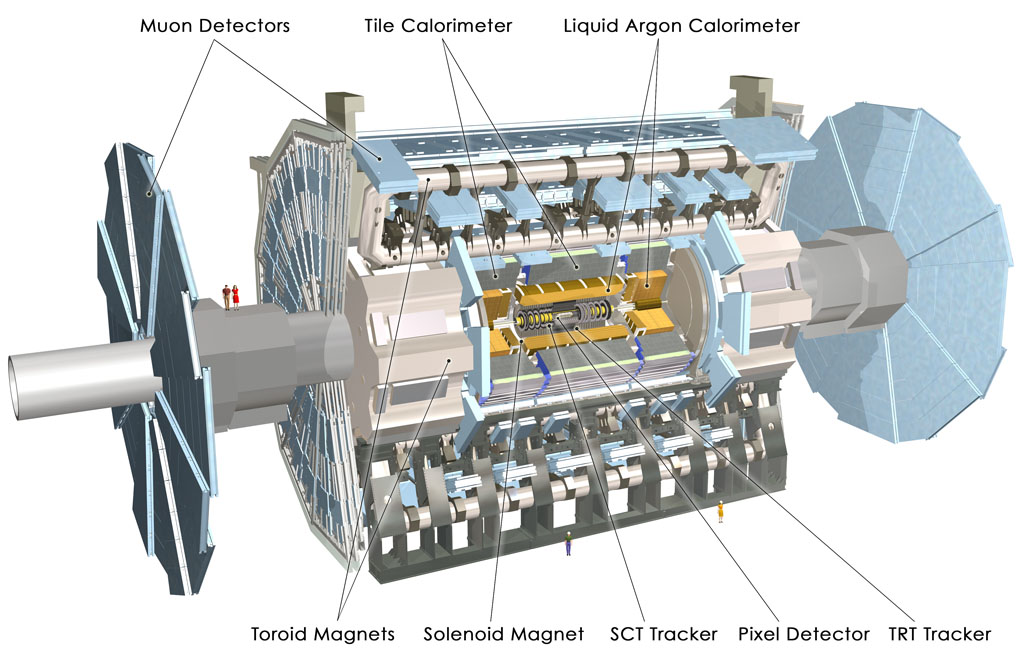
\includegraphics[width=0.85\linewidth]{figures/detector/ATLAS_Silver_White_MK}
\caption{View of the ATLAS detector and its sub-systems}
\label{fig:detector-atlas}
\end{center}
\end{figure}





%-------------------------------------------------------------------------------
\section{Datasets}
\label{sec:data}
\input{sections/datasets}
%-------------------------------------------------------------------------------

%-------------------------------------------------------------------------------
\section{Object and Event Selection}
\label{sec:obj}
\label{sec:gbb-obj}

\subsubsection{Primary Vertex and Track Selection}
The primary hard scattering vertex for the event is chosen as the vertex with the highest $\sum p_{T}^{2}$ where the sum runs over the tracks associated to the vertex. Tracks which are used to determine the primary vertex need to pass the following selection:
\begin{enumerate}
    \item $p_T>$ 0.5 GeV
    \item Number of Pixel hits greater than 1
    \item Number of SCT hits greater than 6
    \item $|d_0|<1$mm, with respect to primary vertex
    \item $|z_0\sin(\theta)|<1$mm, with respect to primary vertex
\end{enumerate}

\subsubsection{Jet Selection}
In this study we use $R$=1.0 calorimeter jets and $R=0.2$ track jets. Calorimeter jets are clustered in $y-\phi$ space using the anti-$k_t$~\cite{Cacciari:2008gp} algorithm with $R=1.0$ reconstructed from topological calorimeter clusters~\cite{TopoClusters} using the local cluster weighting (LCW) algorithm \cite{EndcapTBelectronPion2002} and calibrated to account for the detector response. Track jets are reconstructed clustering inner detector tracks using the anti-$k_t$ algorithm and are required to have at least two tracks.

\noindent The $R = 1.0$ calorimeter jets are groomed using the trimming procedure~\cite{Krohn:2009th}, whereupon the $k_{t}$ subjets ~\cite{Cacciari200657} with $R=0.3$ are discarded if the fractional $p_{T}$ of the subject relative to the whole $R=1.0$ jet satisfies $f_\text{ cut}<0.05$.  

\noindent The $R=0.2$ track jets are subject to the following selection, 
\begin{enumerate}
	\item $p_T>$10 GeV
	\item $|\eta|<2.5$	
	\item The track jet originates from the primary vertex (OriginIndex==0)
\end{enumerate}

\subsubsection{$b$-tagging}

Jets are identified as $b$-jets using the multivariate discriminant $MV2c10$ \cite{btag} which includes impact parameter and secondary vertex information as inputs.  The chosen $MV2c10$ working point corresponds to an average $b$-tagging efficiency of 70\% for $b$-jets in simulated $t\bar{t}$ events.  

\subsubsection{Ghost Association of Jets}

We adopt a robust matching algorithm called ghost association~\cite{area} to associate $R=0.2$ track jets to $R=1.0$ jets. With this method, the 4-vector of the physics object is added to the inputs of the jet clustering algorithm but the object 4-vector has the $p_T$ set to an infinitesimal amount, hence called a ghost.  Jet clustering is then performed. This way, the ghost does not alter the clustering history, but the 4-vectors retain the original object direction and are clustered into a jet if the ghost 4-vector points within the active area of the jet.

\subsubsection{Flavor Labeling of Jets in Simulation}

The flavor content of the track jet is determined by ghost matching truth particles (weakly decaying $B$-hadrons and $c$-hadrons) to the track jet. For each jet, if a $B$-hadron is found to be associated to the jet, then the jet is labeled as a $b$-jet.  If there are no $B$-hadrons but a $c$-hadron is found to be associated to the jet, then the jet is labeled as a $c$-jet. Otherwise, the jet is labeled as a light-flavored jet. 

\subsubsection{Truth Jets}

All final state truth particles (ignoring truth pileup) with mean lifetimes longer than 30 ps, except muons and neutrinos, are used as input to the clustering of truth jets. 

%-------------------------------------------------------------------------------

%-------------------------------------------------------------------------------
\section{Observables}
\label{sec:obs}
\input{sections/observables}
%-------------------------------------------------------------------------------

%-------------------------------------------------------------------------------
\section{Background Estimation}
\label{sec:analysis}
\label{sec:gbb-bkgsub}
\subsection{Flavor Fractions}
Post \btagging, a large fraction of events are backgrounds as shown in Table~\ref{tab:posttaggingflav}. To unfold the data, subtraction of the remnant background is necessary. It is a known problem that the nominal MC flavor fractions could deviate from the true values in data (see e.g.~\cite{ATLAS-CONF-2016-002}). To have good control over the flavor fractions, we seek to estimate the flavor fractions in bins of each observable by fitting the distributions of some variables, which may not be powerful enough to tag individual jets, but are sensitive to the numbers of jets of different flavors. 

\begin{table}[htbp]
\centering
\resizebox{\textwidth}{!}{
\begin{tabular}{|l|l|l|l|l|l|l|l|l|l|}
\hline
Flavor Combination & BB      & BC     & BL     & CB     & CC     & CL     & LB     & LC     & LL     \\ \hline
Flavor Fraction    & 19.01\% & 2.20\% & 34.68\% & 0.39\% & 5.73\% & 17.99\% & 0.37\% & 0.86\% & 18.76\% \\ \hline
\end{tabular}}
\caption{Post $b$-tagging flavor composition in MC. The first letter of the flavor combination is the flavor of the leading jet. The second letter of the combination is the flavor of the sub-leading jet. }
\label{tab:posttaggingflav}
\end{table}


\subsection{$s_{d_{0}}$ as Discriminant Variable }
\label{sec:gbb-sd0}

The long decay length of heavy flavor hadrons make the signed significance of impact parameter $s_{d_{0}}$ of tracks associated to a jet a good discriminating variable. The $s_{d_{0}}$ is defined as 
\begin{equation}
s_{d_{0}} = \frac{d_0}{\sigma(d_0)} \cdot s_{j}
\end{equation}
where $d_{0}$ is the track transverse impact parameter, $\sigma(d_{0})$ is the uncertainty on the $d_0$ measurement, and $s_{j}$ is the sign of $d_{0}$ with respect to the jet axis. The variable $s_j$ is defined as
\begin{equation}
s_{j} = \textrm{sign}\left\{\ \sin\left(\arctan \left( \frac{p_{j,\ y}}{p_{j,\ x}}\right) - \phi_t\right) \cdot d_{0} \ \right\}
\end{equation}
 where $p_{j,\ x}$ and $p_{j,\ y}$ are the $x$ and $y$ components of the jet moments, respectively, and $\phi_{t}$ is the azimuthal angle of the track.
 
For a given track jet, by construction we have at least two tracks as constituents of the jet. %(number of track constituents distributions are shown in Fig.\ref{fig:gbb-ntrk}).
We take the sub-leading $s_{d_{0}}$ of the track (leading means highest value of $|s_{d_{0}}|$, sub-leading is second largest, etc.) as \subsdzero and build templates of different flavors using this variable to fit and derive the flavor fractions from data.   The second highest $s_{d_{0}}$ is used because it is less likely the result of mis-measured track parameters for non-$b$-jets. For illustration of the impact parameter significance please refer back to Fig.\ref{fig:reco-trkdef}.


%\begin{figure}[htbp]
%  \centering
% 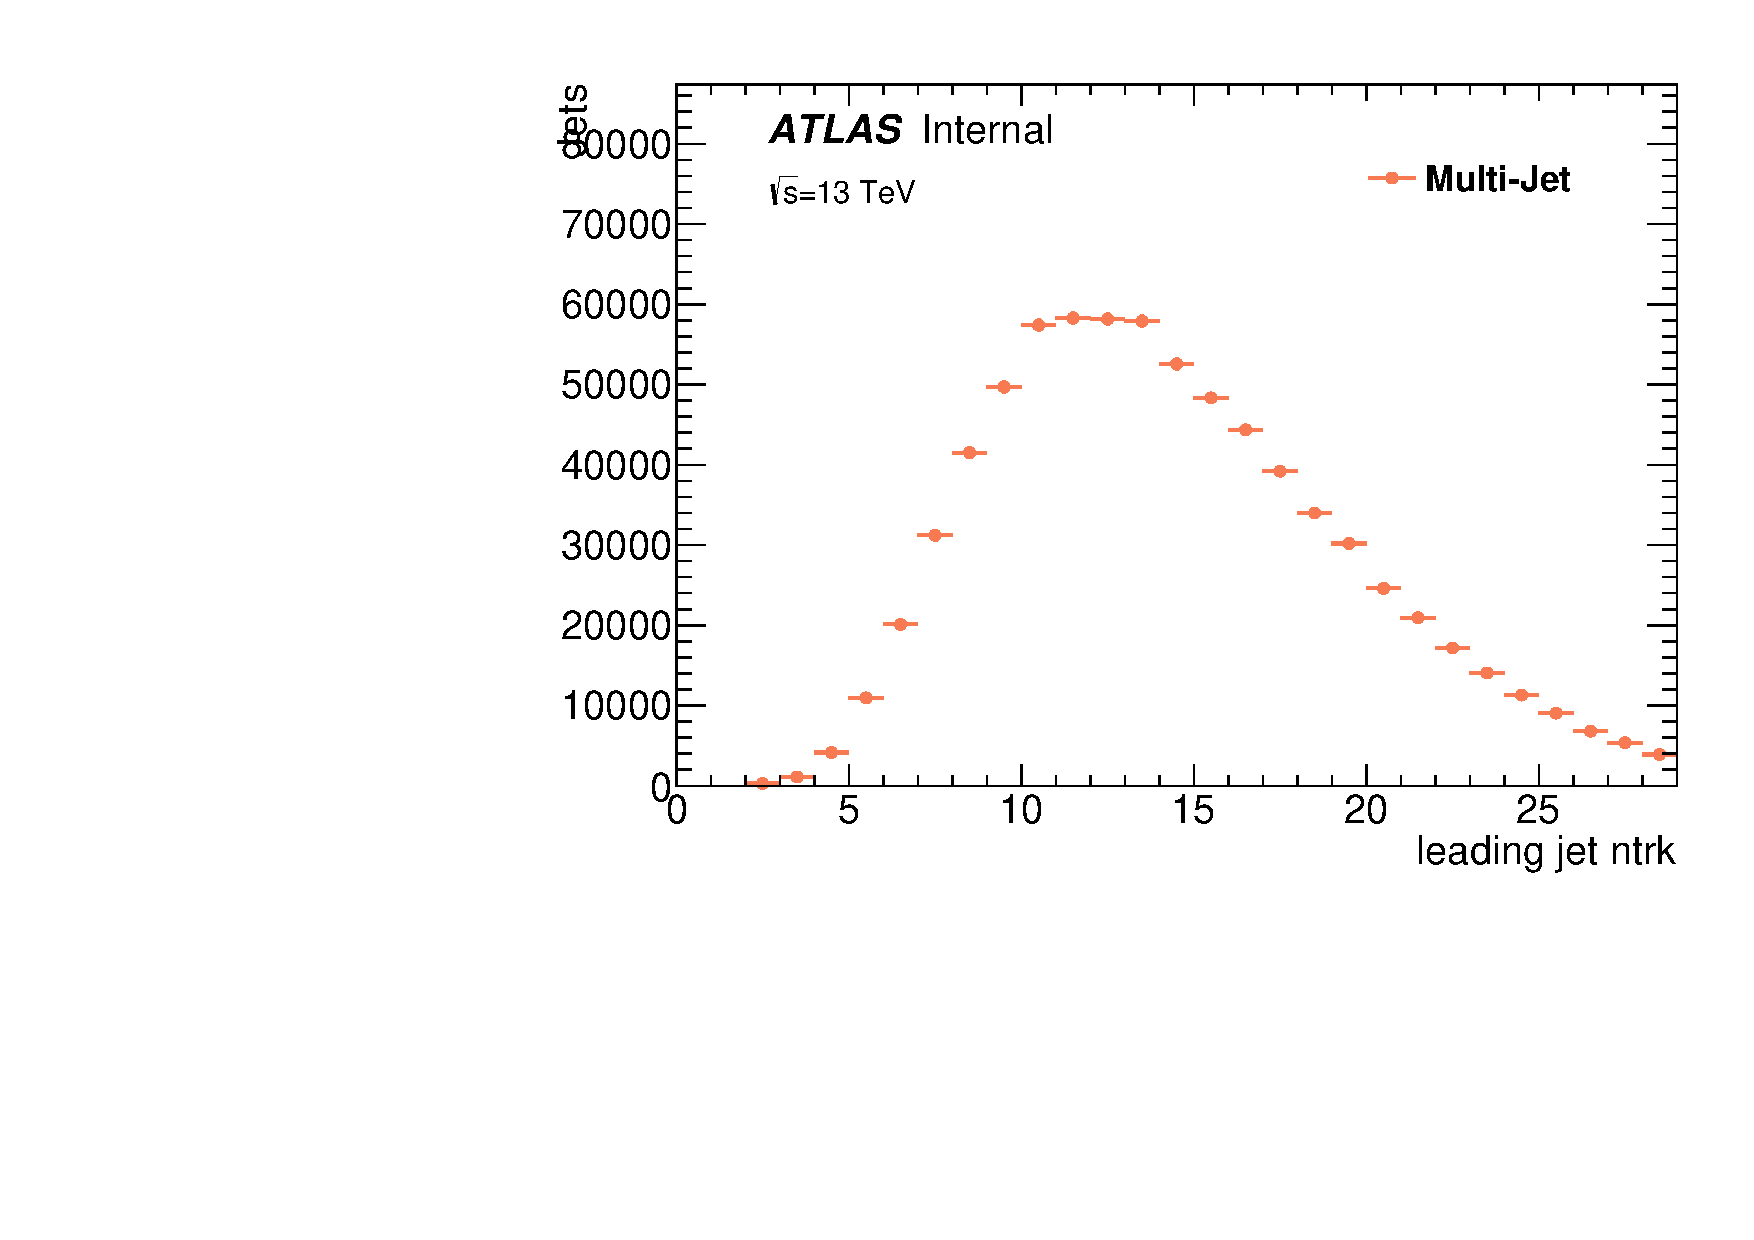
\includegraphics[width=0.48\textwidth]{figures/gbb/Leading_trkjet_ntrk_PostTag.pdf}
% 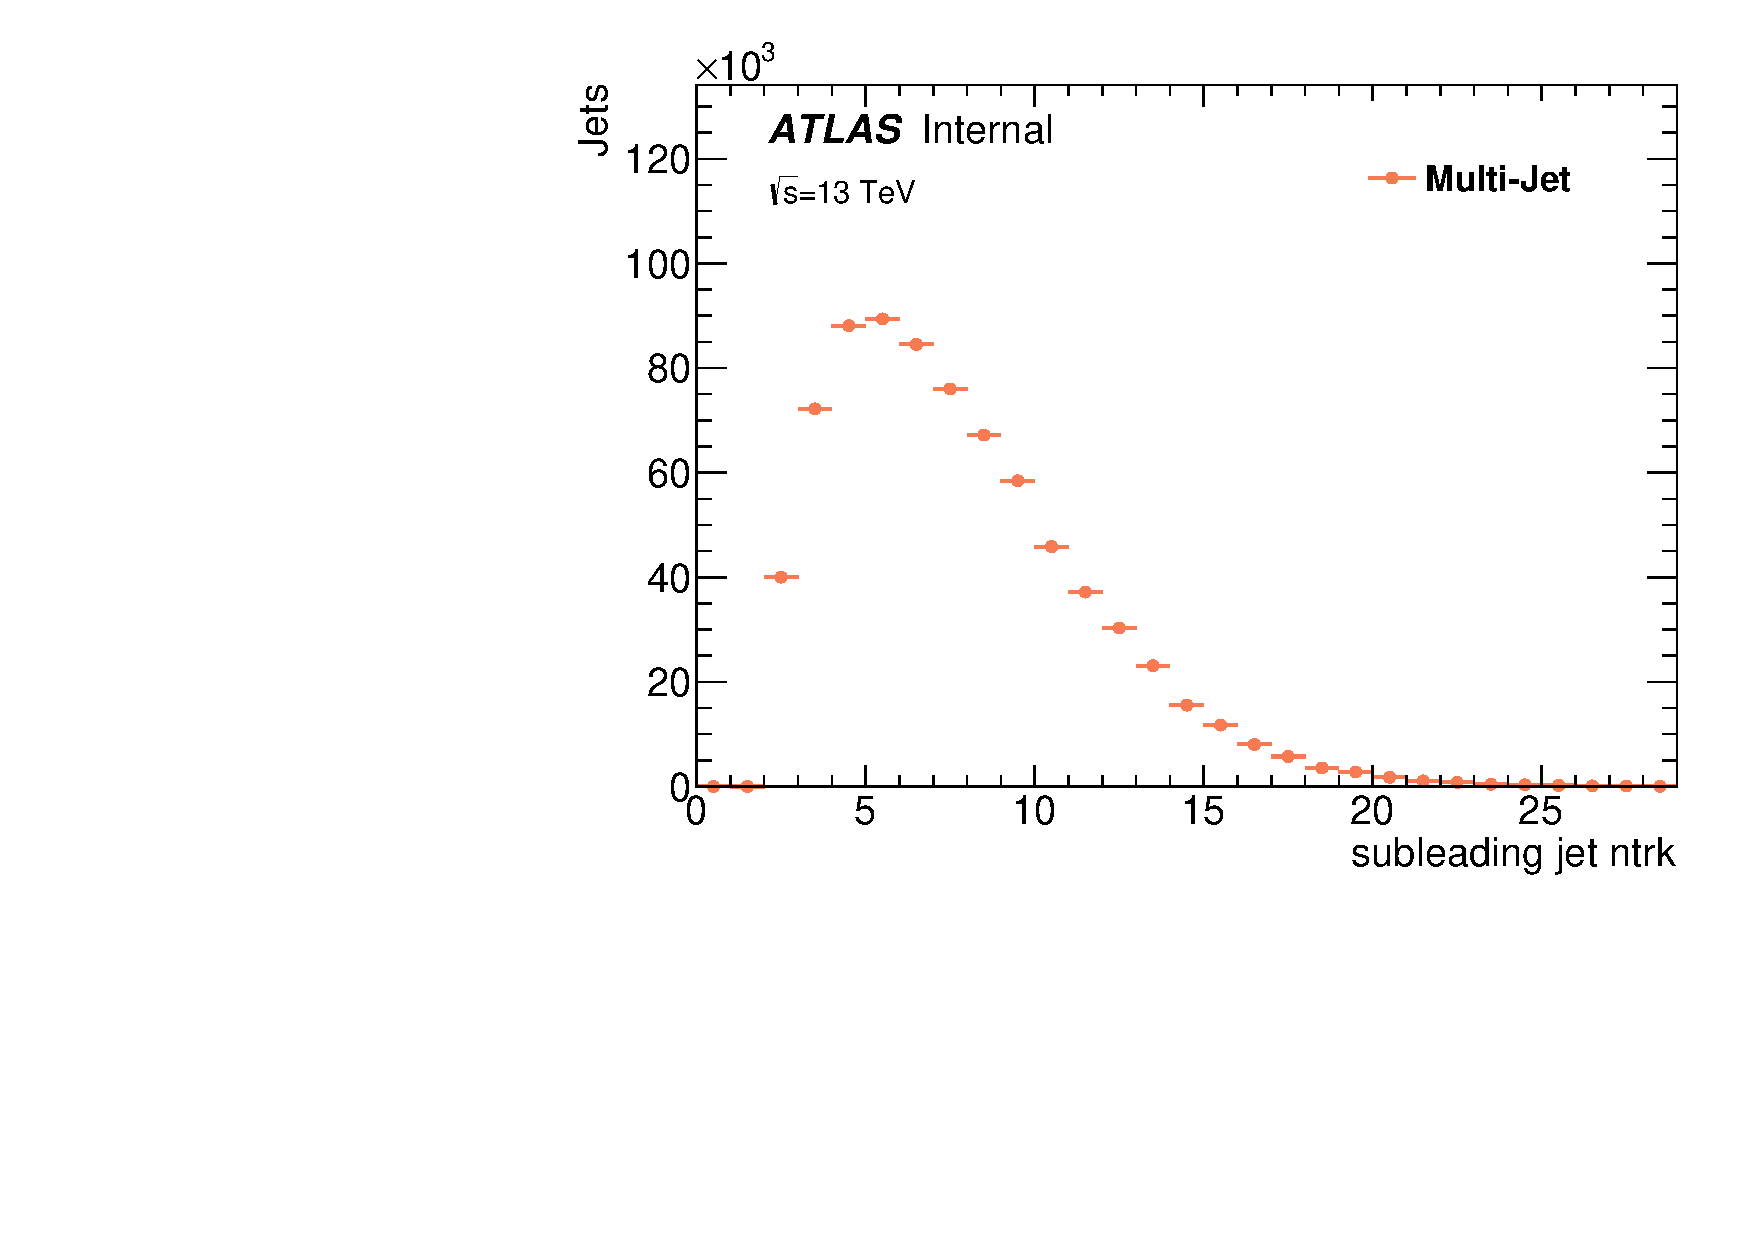
\includegraphics[width=0.48\textwidth]{figures/gbb/SubLeading_trkjet_ntrk_PostTag.pdf}\\
%\caption{The number of track distribution for leading (left) and sub-leading (right) track jets in MC prediction}
%  \label{fig:gbb-ntrk}
%\end{figure}


%%%%%%%%%%%%%%%%%%%%%%%%%%%%%%%%%%%%%%%%%%%%%%%%%

\subsection{Binned Maximum Likelihood Estimation}

An $m$ flavor component template fit ($m = 3$ for the fit we perform) is carried out by maximizing a binned likelihood function defined as $\mathcal{L} = \prod _{i=1} ^n p(y_i| \vec{\theta})$, where $\vec{\theta} \in \mathbb{R}^m$ denotes the number of events from each flavor component, $n$ is the number of bins we are fitting and $y_i$ is the number of data events in bin $i$. The assumption of $p(y_i|\vec{\theta})$ is Poisson distribution: 
\begin{equation}
p(y_i|\vec{\theta}) = \frac{\exp{(-\vec{\theta} \vec{\cdot x_i)}} {(\vec{\theta}} \vec{\cdot x_i})^{y_i}}{y_i !}, 
\end{equation}
where $\vec{x_i}=(x_{i1}...,x_{ij}...,x_{im}) \in \mathbb{R}^m$ is a vector, and each component denotes the $i^{th}$ bin value in the normalized templates for the $j^{th}$ flavor ($b$, $c$ and light).   We determine the flavor fractions by finding the $\vec{\theta}$ that maximizes $\mathcal{L}$. The fit is carried out by the MIGRAD function of the MINUIT package. 

%%%%%%%%%%%%%%%%%%%%%%%%%%%%%%%
\subsection{\subsdzero Templates }
\label{sec:gbb-subdzerotemplates}

The flavor contents of the two $R=0.2$ jets in a $R=1.0$ jet are correlated. 
Tagging one of the $b$ jets increases the probability of the other track jet 
being a $b$ jet. Therefore, we should not treat the flavor 
contents of the two jets independently and thus must take into account both jets 
flavors simultaneously when fitting. On the other hand, given the flavors of the 
two $R= 0.2$ jets, their \subsdzero values are not correlated, as shown in Table \ref{tab:sd0cor}. 
Therefore, we can derive the flavor fractions by fitting simultaneously the 
1-dimensional \subsdzero distributions of the leading and sub-leading jets
 using templates derived from all of the possible 2-jet flavor pair 
combinations. This is essentially a Naive Bayes approximation, i.e. assuming the joint 
2-D probability density is the product of the two 1-D probability density
 $p(\subsdzero(j1), \subsdzero(j2)) = p(\subsdzero(j1))p(\subsdzero(j2))$.

\begin{table}[htbp]
\centering
\begin{tabular}{|r|r|r|r|}
\hline
\centering
Flavor Combination & \subsdzero Correlation Factor\\
\hline
BB & 0.7\% \\
BL & 0.4\% \\
BC & -2.2\% \\
LB & 3.9\%\\
LL & 0.3\%\\
LC & 0.8\%\\
CB & -0.3\% \\
CL & 0.5\% \\
CC & -4.1\% \\

\hline
\end{tabular}%
\caption{Correlation factor between the \subsdzero values of the two R = 0.2 jets.}
\label{tab:sd0cor}
\end{table}%

There are in total nine different ordered flavor pairs: BB, BL, BC, CB, CL, CC, 
LB, LC and LL such that the first flavor is that of the leading track jet and 
the second is that of the other track jet. Many of these components are very small 
for us to fit their contributions correctly as show in Table~\ref{tab:posttaggingflav}. 
Therefore, starting with BL, CL templates, we merge other templates to these templates
to form B-like and C/L-like templates. The metric we use for determining the similarity 
between two distributions is: $S=\frac{1}{2}\int \frac{(p_1(x)-p_2(x))^2}{p_1(x)+p_2(x)}$, 
where $p_1(x)$ and $p_2(x)$ are two different distributions. 
Based on calculation, we merge the BC template with the BL 
template, and other components into CL as seen in 
Table \ref{tab:overlap-unmerged}. The merged templates are 
presented in Figure \ref{fig:gbb-templates} and the separation powers estimated by the same metric are 
presented in Table \ref{tab:overlap-merged}. 
We show the full set of templates in bins of the observables we are interested in 
measuring in Appendix~\ref{sec:gbb-app-sd0templates}. 

It is noteworthy that the statistics of our Monte Carlo samples is low.
Presumably, a double $b$-tagging strategy would be preferable as it could filter 
out most of the background processes.
However, double $b$-tagging strategy would also yield background templates with large 
statistical fluctuations. In Fig. \ref{fig:gbb-template-leadtight-medium} the comparison 
of the templates derived from single $b$-tagging and double $b$-tagging (at 70\% $b$-
efficiency for both jets) in one bin of $\Delta R$ is shown. The considerable statistical uncertainties ($\geq 10\%$ relative uncertainty per bin in template)
of double $b$-tagging strategy lead us to use single $b$-tagging strategy instead. 


\begin{table}[htpb]
\centering
\begin{tabular}{|l|l|l|l|l|}
\hline
   & BL   & CL    & BB   \\ \hline
BC & 0.02 & 0.08  & 0.11 \\ \hline
CC & 0.09 & 0.03  & 0.14 \\ \hline
LC & 0.07 & 0.05  & 0.12 \\ \hline
LB & 0.17 & 0.12  & 0.05 \\ \hline
CB & 0.19 & 0.14  & 0.08 \\ \hline
LL & 0.02 & 0.01  & 0.17 \\ \hline
BB & 0.16 & 0.21  & 0    \\ \hline

\end{tabular}
\caption{Templates similarity calculated using the metric $S=\frac{1}{2}\int \frac{(p_1(x)-p_2(x))^2}{p_1(x)+p_2(x)}$ for un-merged templates. Given two distributions $p_1(x)$ and $p_2(x)$, the metric returns 0 if they are exactly the same and returns 1 if there is no overlap between them.}
\label{tab:overlap-unmerged}
\end{table}



\begin{table}[htpb]
\centering
\begin{tabular}{|l|l|l|l|l|}
\hline
    & B    & L+C    & BB   \\ \hline
B   & 0    & 0.04  & 0.16 \\ \hline
L+C & 0.04 & 0     & 0.17 \\ \hline
BB  & 0.16 & 0.17  & 0    \\ \hline

\end{tabular}
\caption{Templates similarity calculated using the metric $S=\frac{1}{2}\int \frac{(p_1(x)-p_2(x))^2}{p_1(x)+p_2(x)}$ for merged templates. Given two distributions $p_1(x)$ and $p_2(x)$, the metric returns 0 if they are exactly the same and returns 1 if there is no overlap between them.}
\label{tab:overlap-merged}
\end{table}


\begin{figure}[htbp]
  \centering
 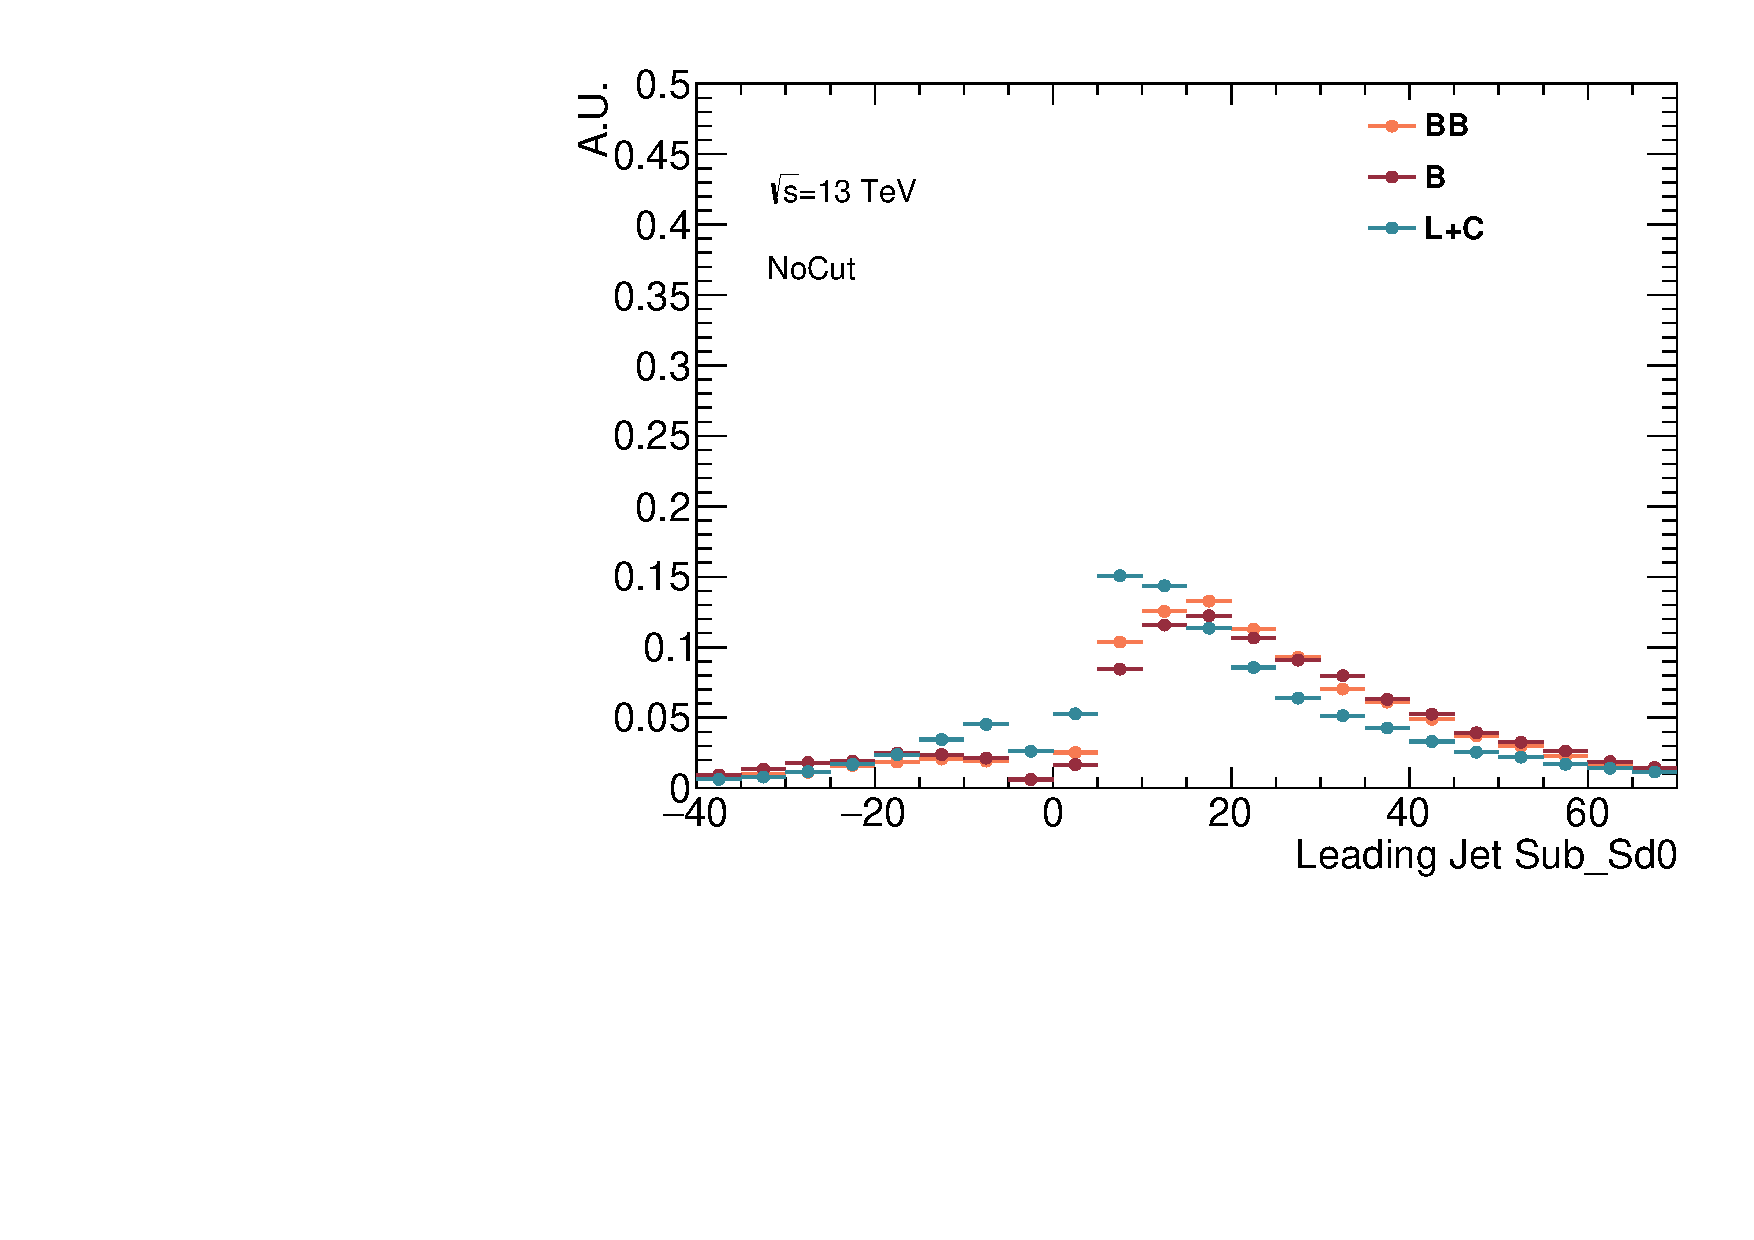
\includegraphics[width=0.48\textwidth]{figures/gbb/Sub_Sd0_Fits/Canv_FitTemplate_Inclusive_x.pdf}
 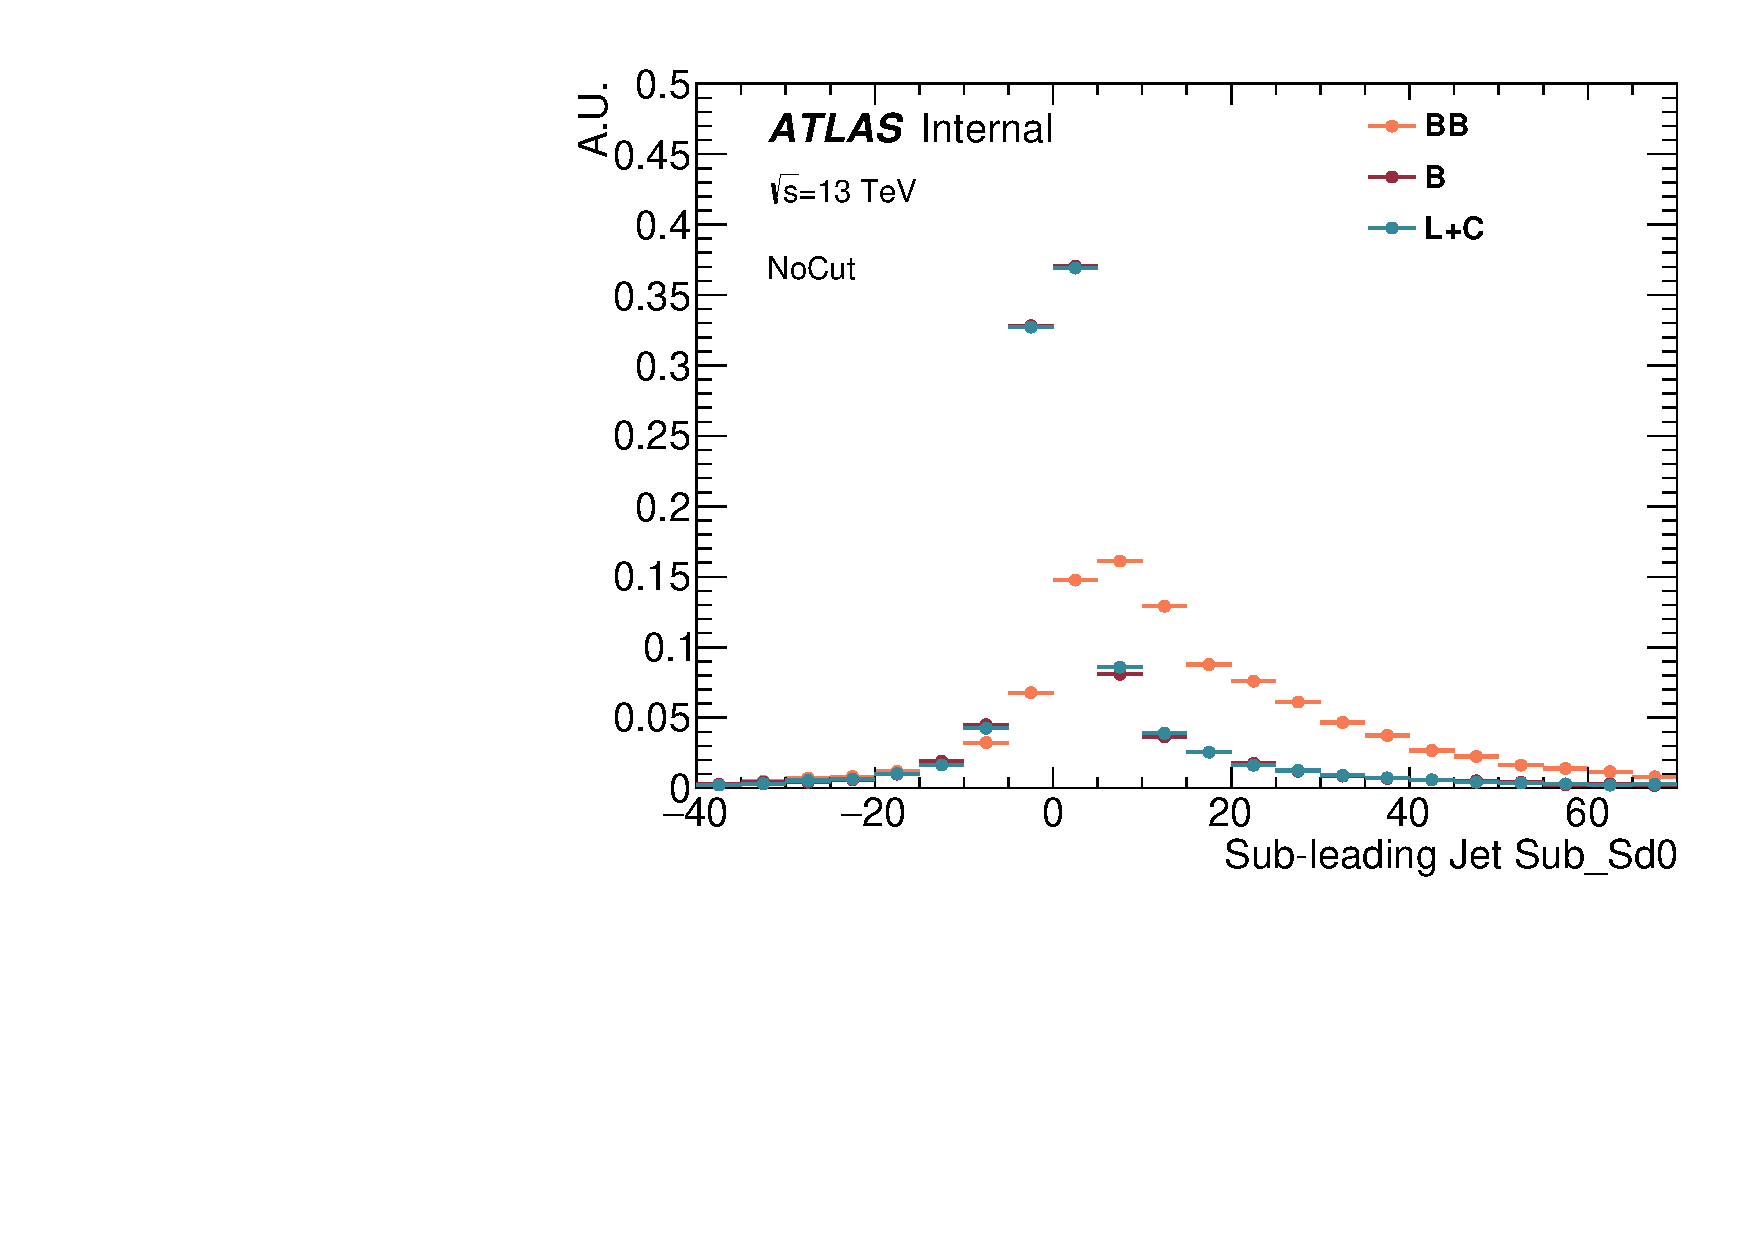
\includegraphics[width=0.48\textwidth]{figures/gbb/Sub_Sd0_Fits/Canv_FitTemplate_Inclusive_y.pdf}\\
\caption{The merged \subsdzero templates (inclusive) for leading (left) and sub-leading (right) track jets.}
  \label{fig:gbb-templates}
\end{figure}


\begin{figure}[htbp]
  \centering
 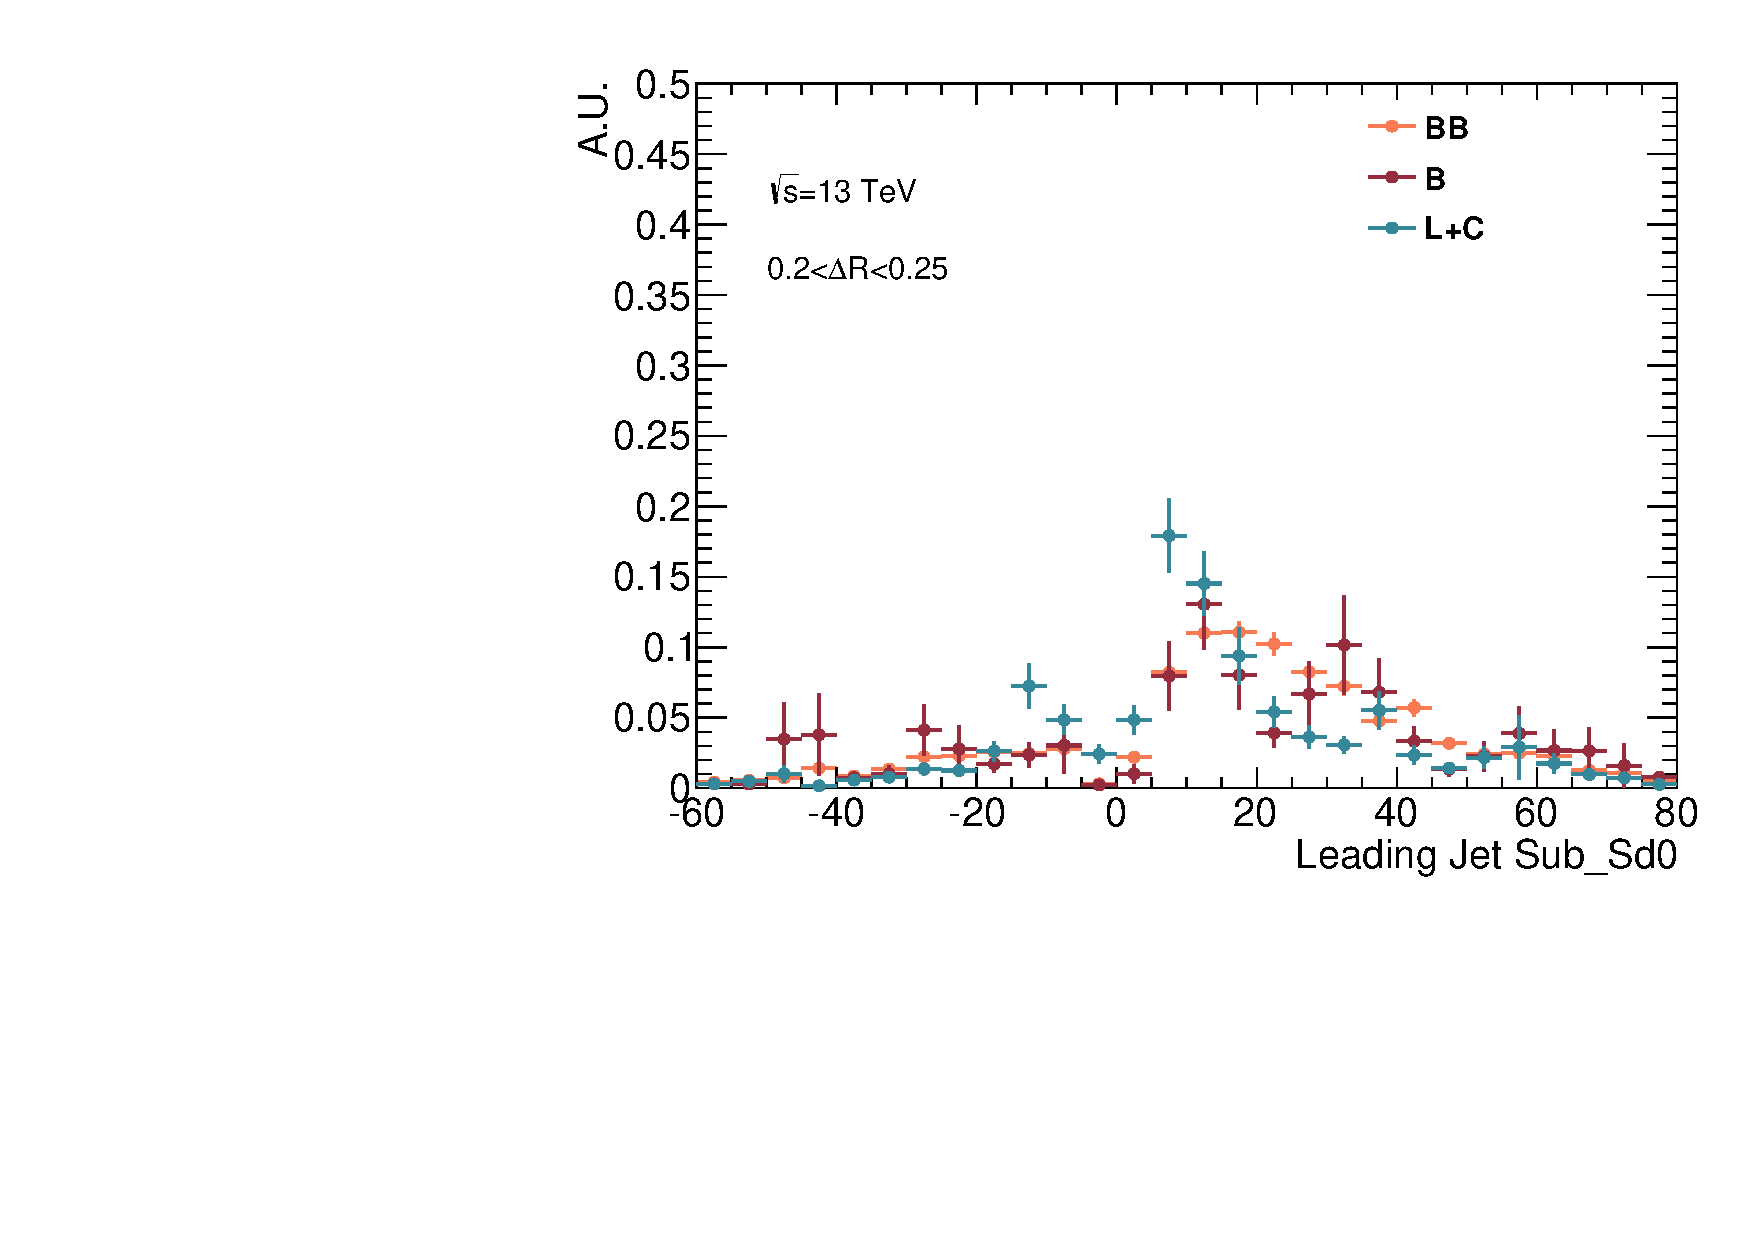
\includegraphics[width=0.48\textwidth]{figures/gbb/Canv_FitTemplate_medium.pdf}
 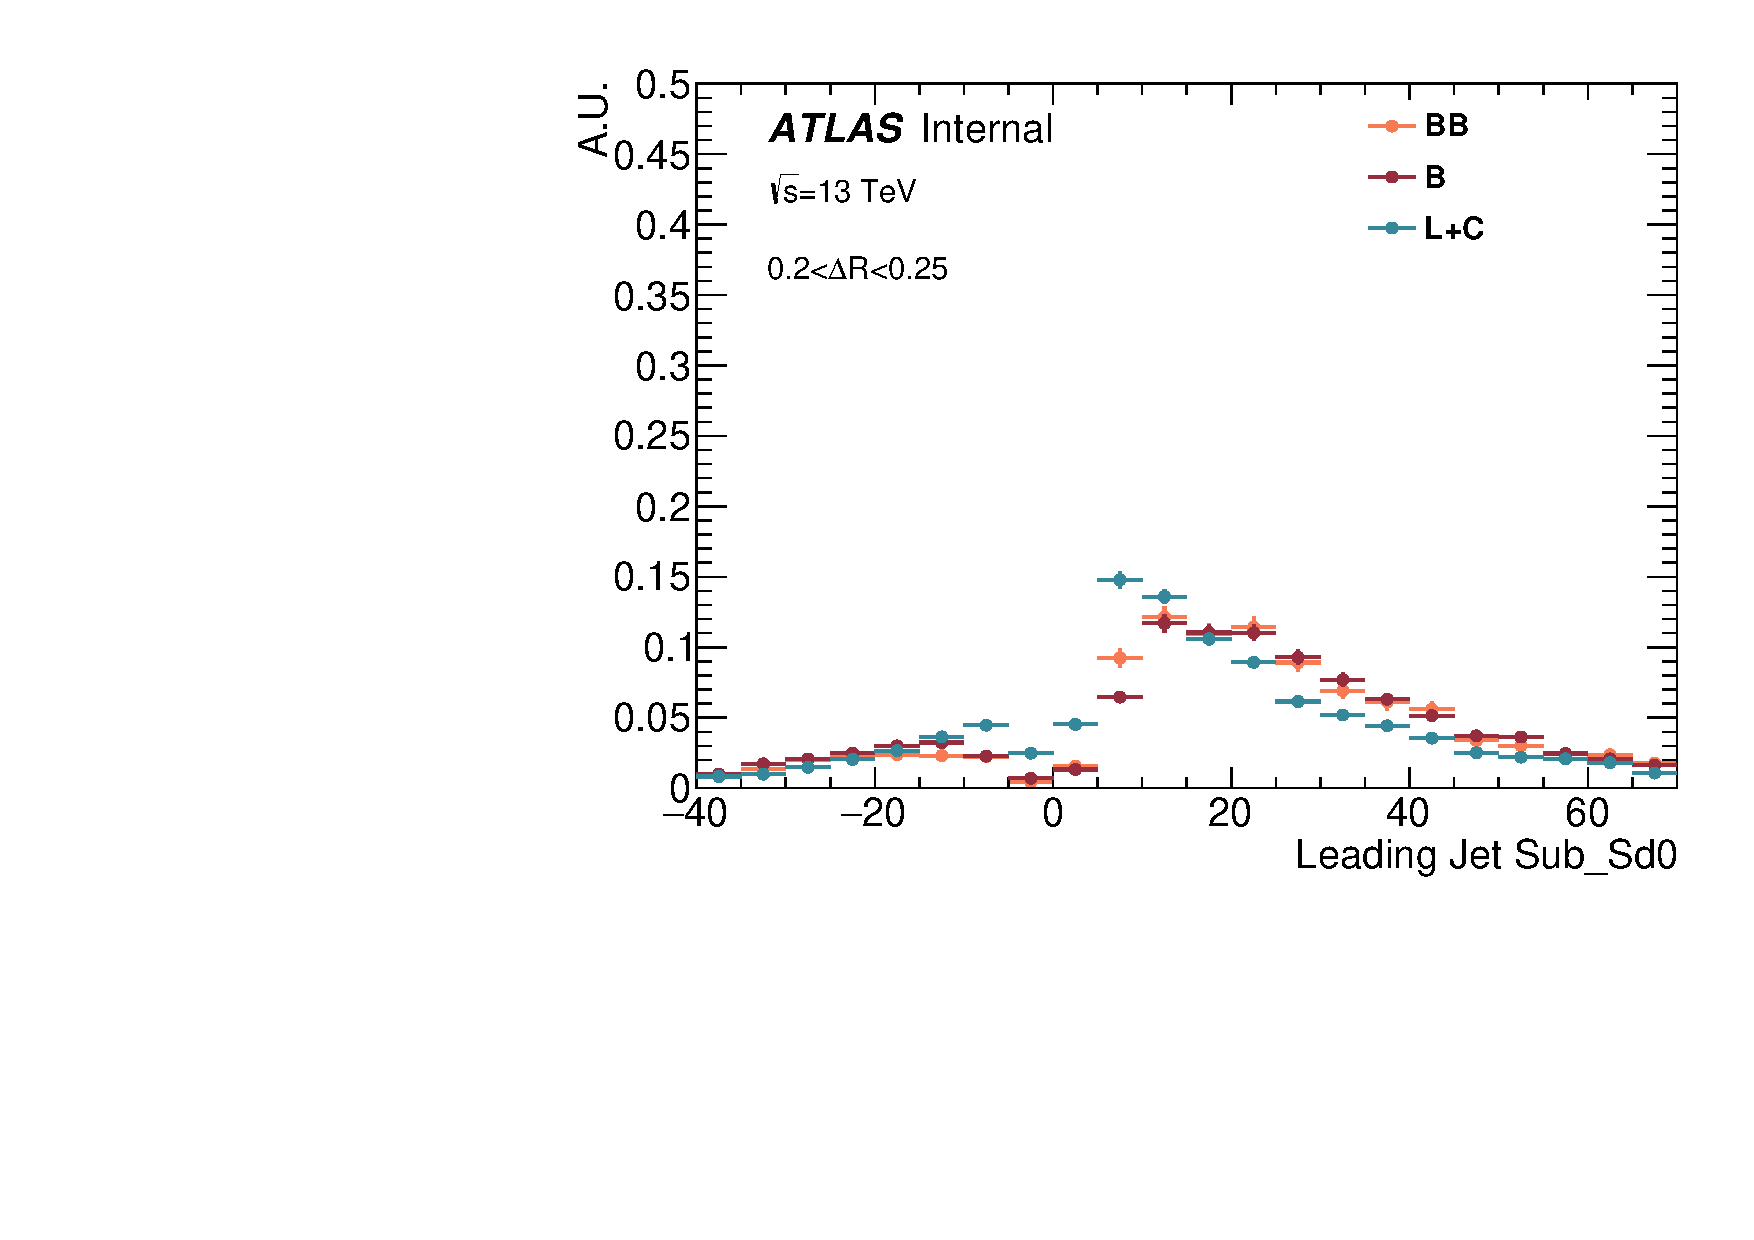
\includegraphics[width=0.48\textwidth]{figures/gbb/Sub_Sd0_Fits/Canv_FitTemplate_02-DeltaR-025_LpT_INF_SpT_INF_x.pdf}\\
\caption{The merged \subsdzero templates for leading track jets of events with $0.2<\Delta R<0.25$ for double $b$-tagging at 70\% eff WP (left) and single $b$-tagging (right). Post double $b$-tagging the statistics of background templates is too low.}
 \label{fig:gbb-template-leadtight-medium}
\end{figure}


%%%%%%%%%%%%%%%%%%%%%%%%%%%%%%%
\subsection{Systematic Uncertainty from Flavor Fraction Fits and Validation Checks}
\label{sec:gbb-sub_systematics}

Separate fits are performed for all the $\pm 1\sigma$ variations of detector systematics listed in Section~\ref{sec:gbb-systs:exp} and propagated through fits. In addition, a number of systematic uncertainties specific for the flavor fraction fits are taken into account for the background determination of the nominal fit:

\begin{enumerate}
  \item \textbf{Data and MC statistical uncertainties:} The fit statistical uncertainties are taken directly from the errors from the MINUIT fitting package and propagated to unfolding.
  \item \textbf{Fit range:} The nominal flavor fraction fit is performed in \subsdzero$\in[-40, 70]$. To avoid having the potential tail mis-modeling of \subsdzero affects the result, fits are separately performed excluding the tails on the left $[-40, -30]$ and right side $[60, 70]$ of the \subsdzero distributions. The $b\bar b$ fitted fraction differences between the left/right-excluded fits and the nominal fit are propagated to unfolding machinery as one source of uncertainty. 
  \item \textbf{Template merging scheme:} The merge of small components to form aggregated templates essentially fixes the relative fractions of these components. The systematic uncertainties caused by the merging scheme is estimated by varying the contribution of each merged component up and down by a factor of two. The template fits are performed for each of these variations. In total $8\times 2 =16$ such variations are propagated to unfolding.
  \item \textbf{Alternative discriminants:} The robustness of the choice using \subsdzero as our fitting templates is checked against another choice using the leading and third-leading $s_{d0}$ value of the track jets, which we define as \sdzero and \subsubsdzero respectively. Note that fitting with these two different variables serves only as a closure check for different background modeling. The difference of fitted flavor fractions are not propagated as a systematic uncertainty associated with unfolding.
  \item \textbf{Fitting with \pt parameterized templates:} The nominal flavor fraction fit with inclusive \subsdzero templates are checked against fitting templates parameterized with track jets \pt. For each bin of observable, the flavor fraction fit is performed in four bins of leading (J1) and sub-leading (J2) track jet \pt: $(p_T(J1), p_T(J2))$. The four bins are $(p_T(J1)<200$~$\GeV, p_T(J2)<80$~$\GeV)$, $(p_T(J1)>200$~$\GeV, p_T(J2)<80$~$\GeV)$, $(p_T(J1)<200$~$\GeV, p_T(J2)>80$~$\GeV)$ and $(p_T(J1)>200$~~$\GeV, p_T(J2)>80$~$\GeV)$. The cross check is performed to check closure. The difference of fitted flavor fractions are not propagated as a systematic uncertainty associated with unfolding.
  \item \textbf{Kinematic re-weighting:} After the event selection, there are mild disagreements between data and MC of jet kinematic properties. The impact of the disagreement on the final results is explored by re-weighting the MC, event-by-event, by the ratio of the two dimensional leading and sub-leading track jets \pt and $\eta$ distributions between MC and data post \btagging as shown in Fig.~\ref{fig:gbb-reweightmap}. The mis-modeling could arise from the overall di-jet cross section, $R=1.0$ ghost matching efficiency and $b$-tagging efficiency as a function of \pt in the particular event topology. The data and MC comparison for the \pt of the $R=1.0$ and track jets are shown after applying $b$-tagging with and without kinematics re-weighting in Fig.~\ref{fig:gbb-pT_largeR},\ref{fig:gbb-pT_leadtrkjets},\ref{fig:gbb-pT_subtrkjets}. We do not find the re-weighting affects the flavor fit in any significant way and hence do not apply the re-weighting for the nominal results and the difference of fitted flavor fractions are not propagated as a systematic uncertainty associated with unfolding.

%\ref{fig:gbb-eta_largeR} \ref{fig:gbb-eta_leadtrkjets},\ref{fig:gbb-eta_subtrkjets}. The effects of applying kinematics re-weighting is checked. A cross check is performed fitting data with templates derived from reweighted sample.

\end{enumerate}

\begin{figure}[htbp]
  \centering
 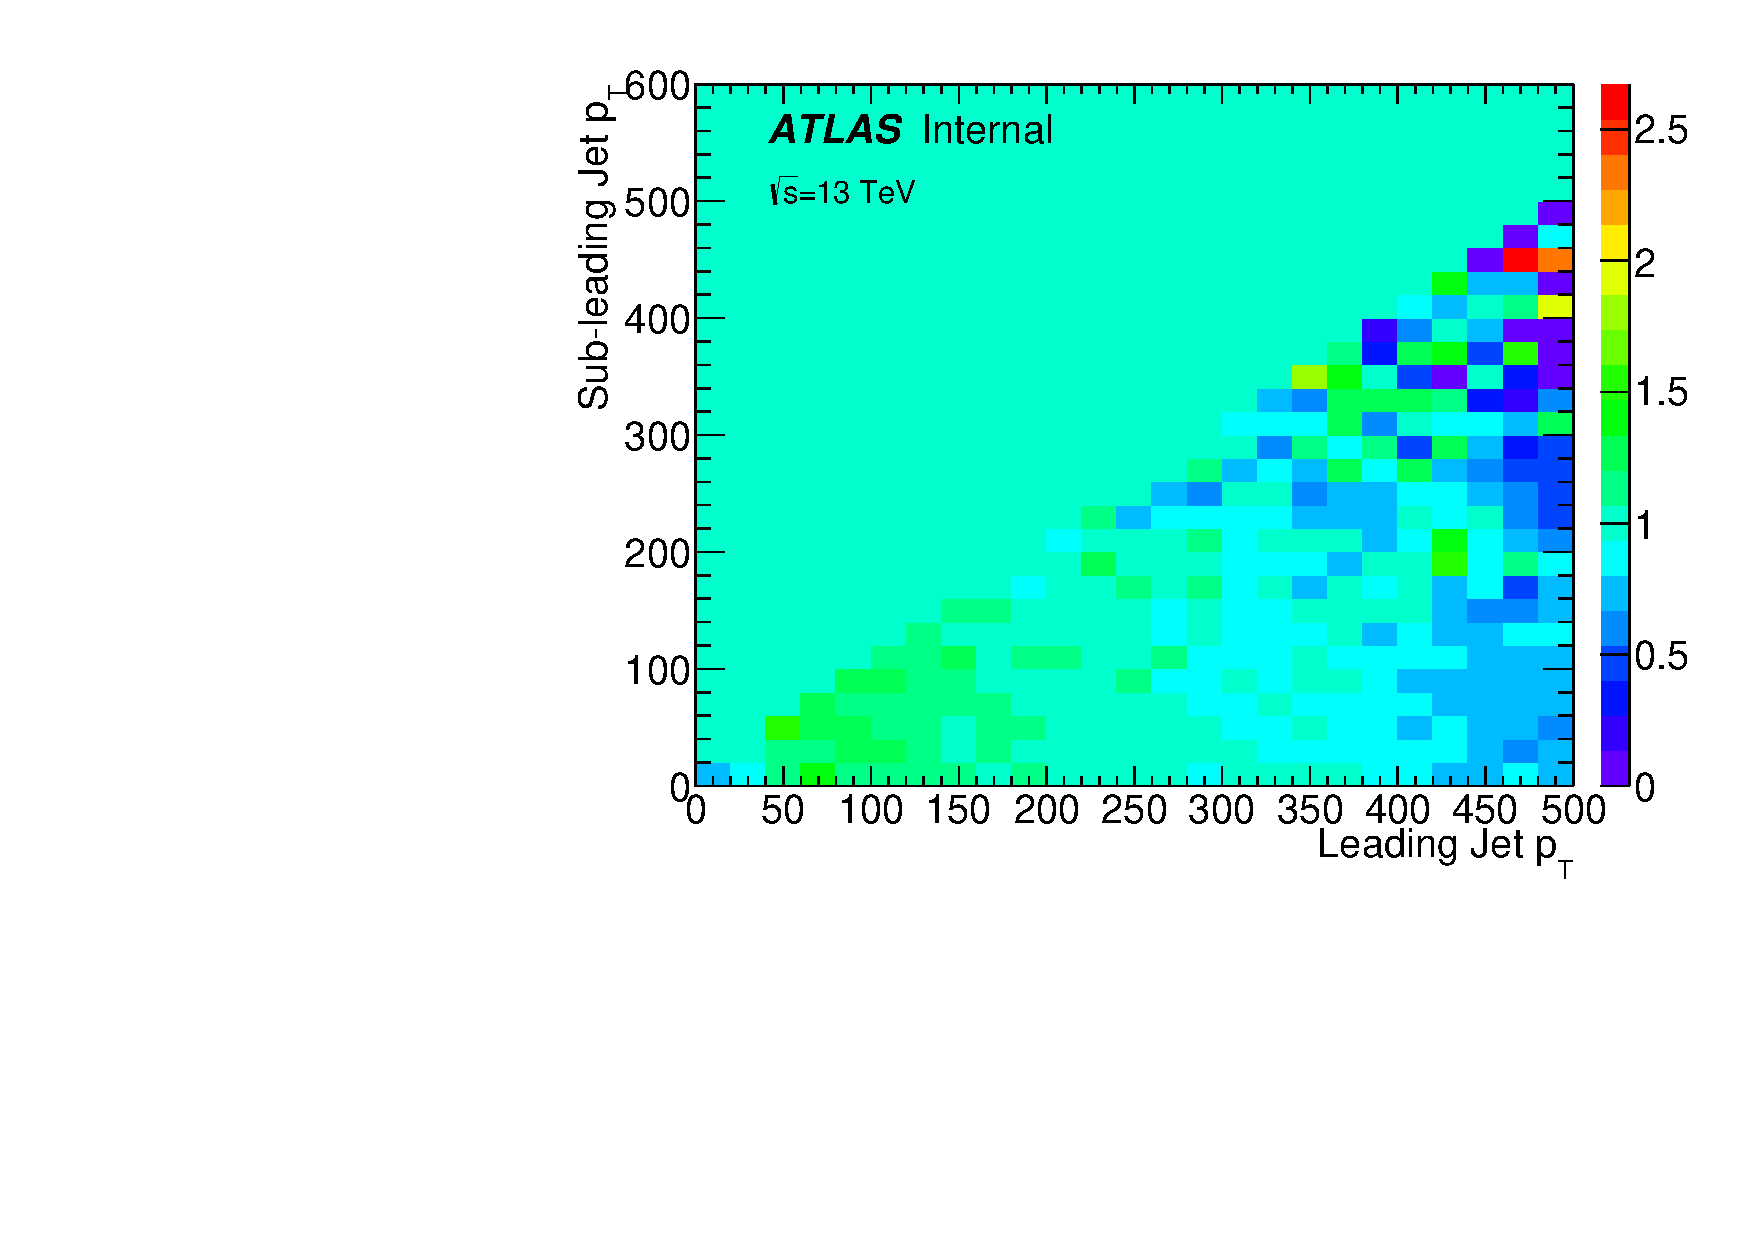
\includegraphics[width=0.6\textwidth]{figures/gbb/pTReweightMap.pdf}
\caption{The re-weighting factor applied to MC as a function of leading and sub-leading track jet \pt.}
  \label{fig:gbb-reweightmap}
\end{figure}


\begin{figure}[htbp]
  \centering
 %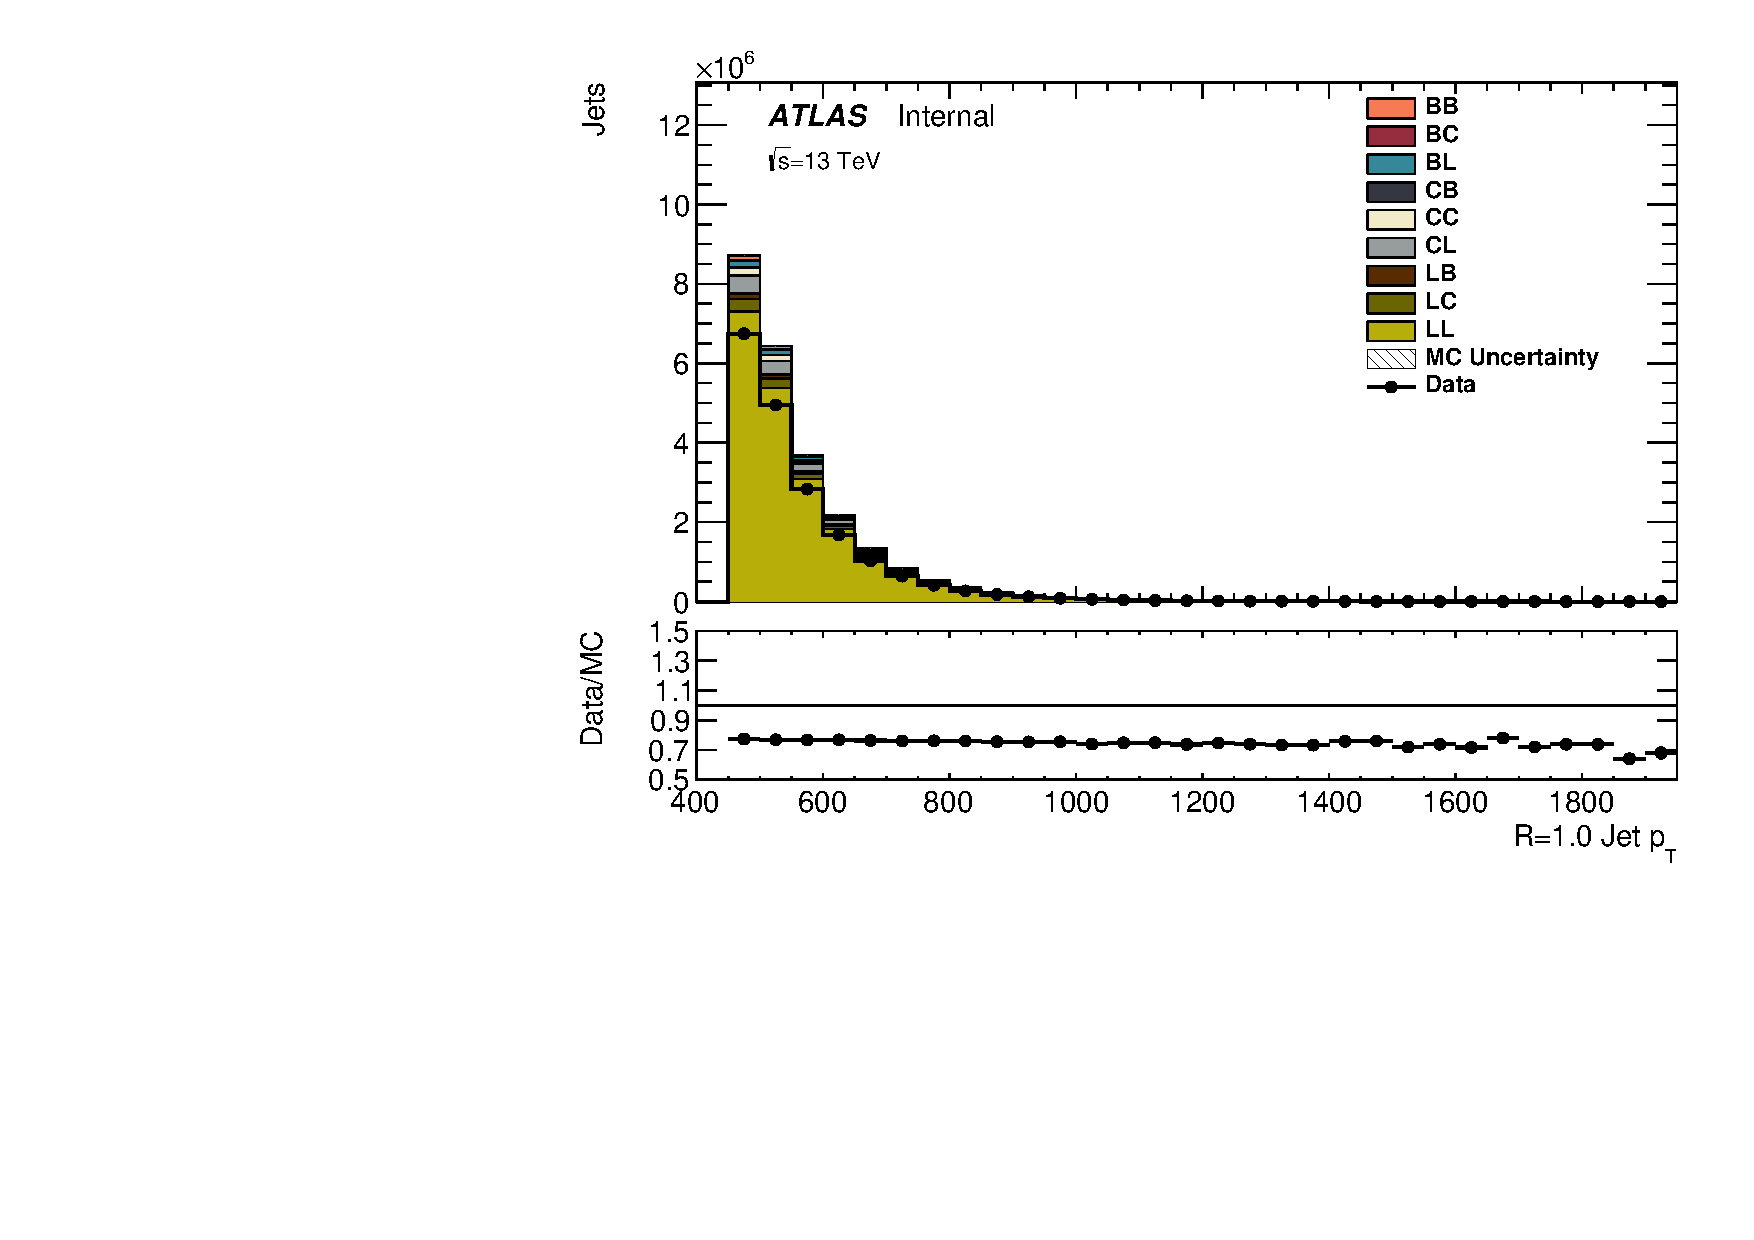
\includegraphics[width=0.38\textwidth]{figures/gbb/LargeRJet_pT_NoReweight.pdf}
 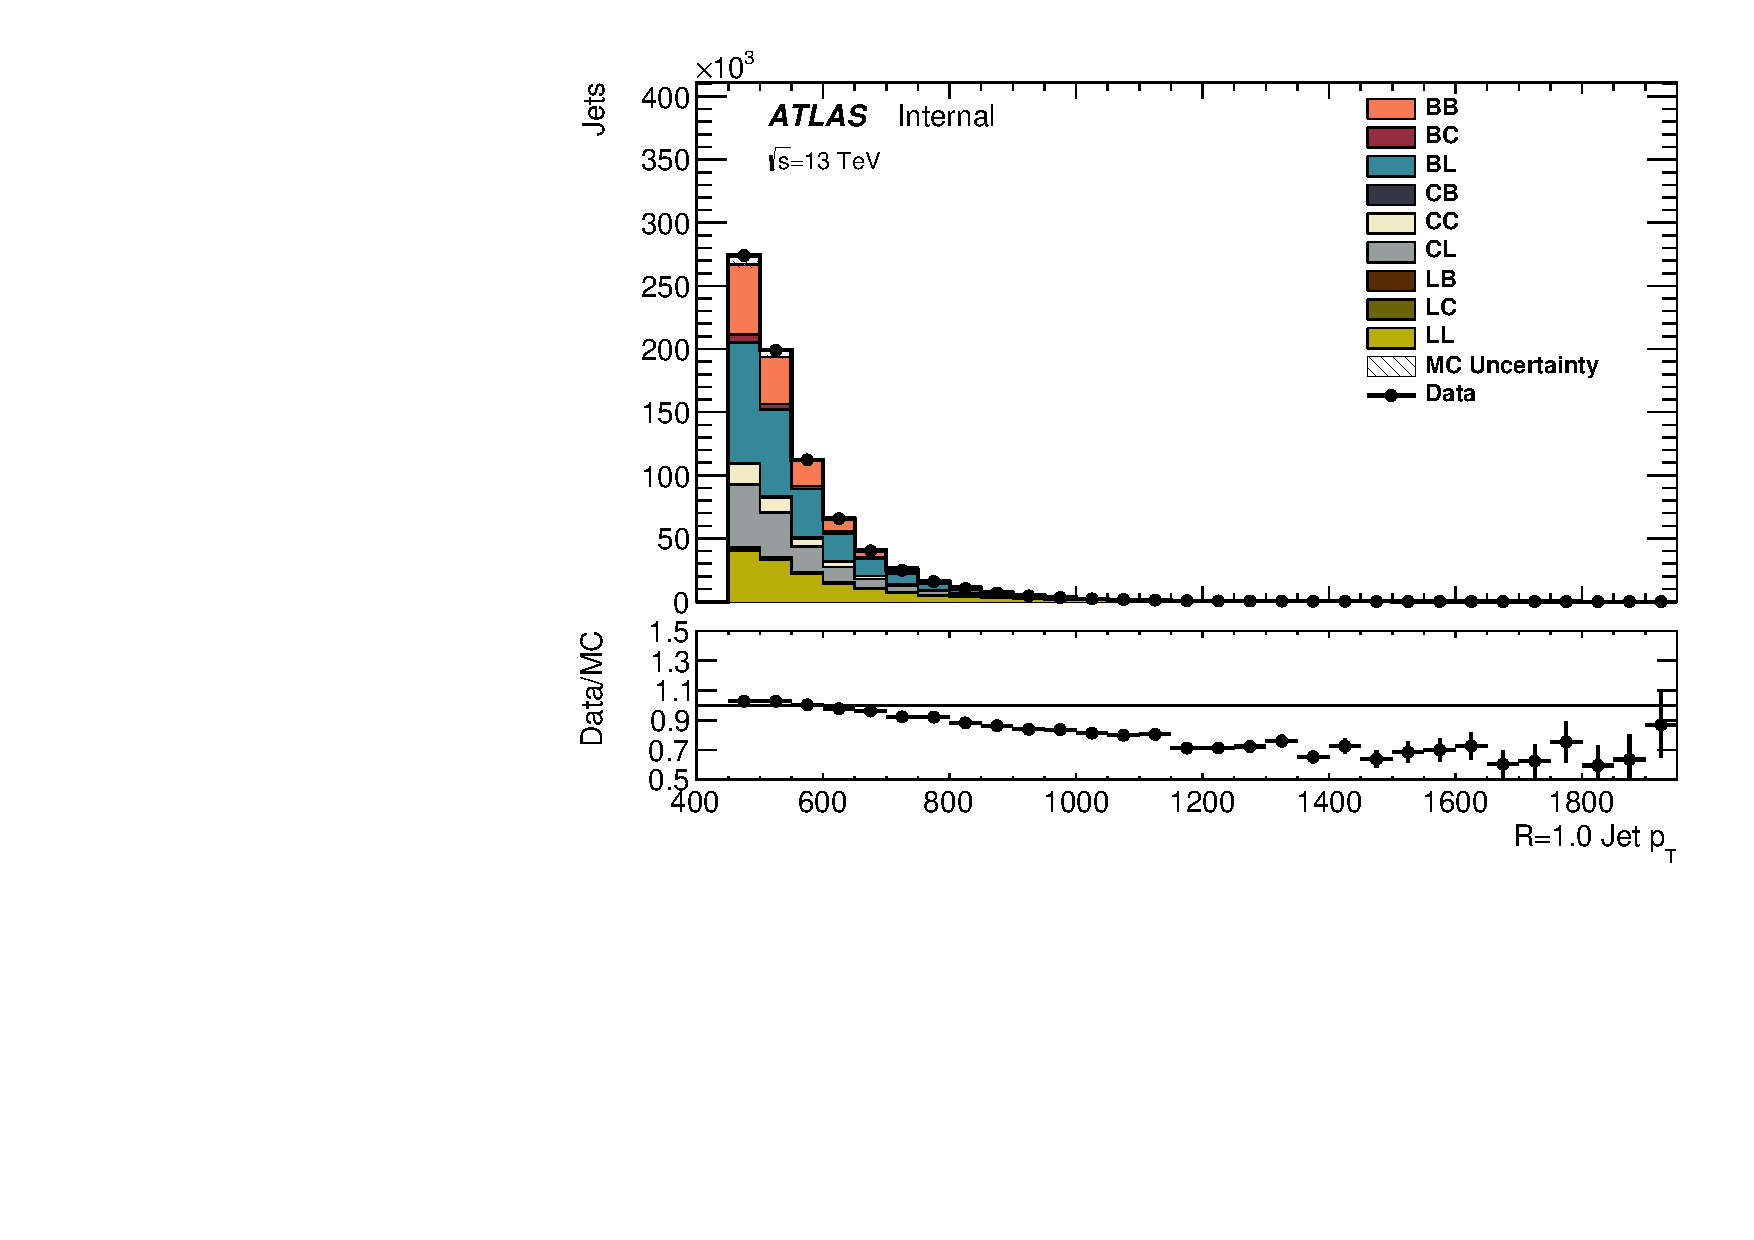
\includegraphics[width=0.38\textwidth]{figures/gbb/LargeRJet_pT_PreReweight.pdf}
 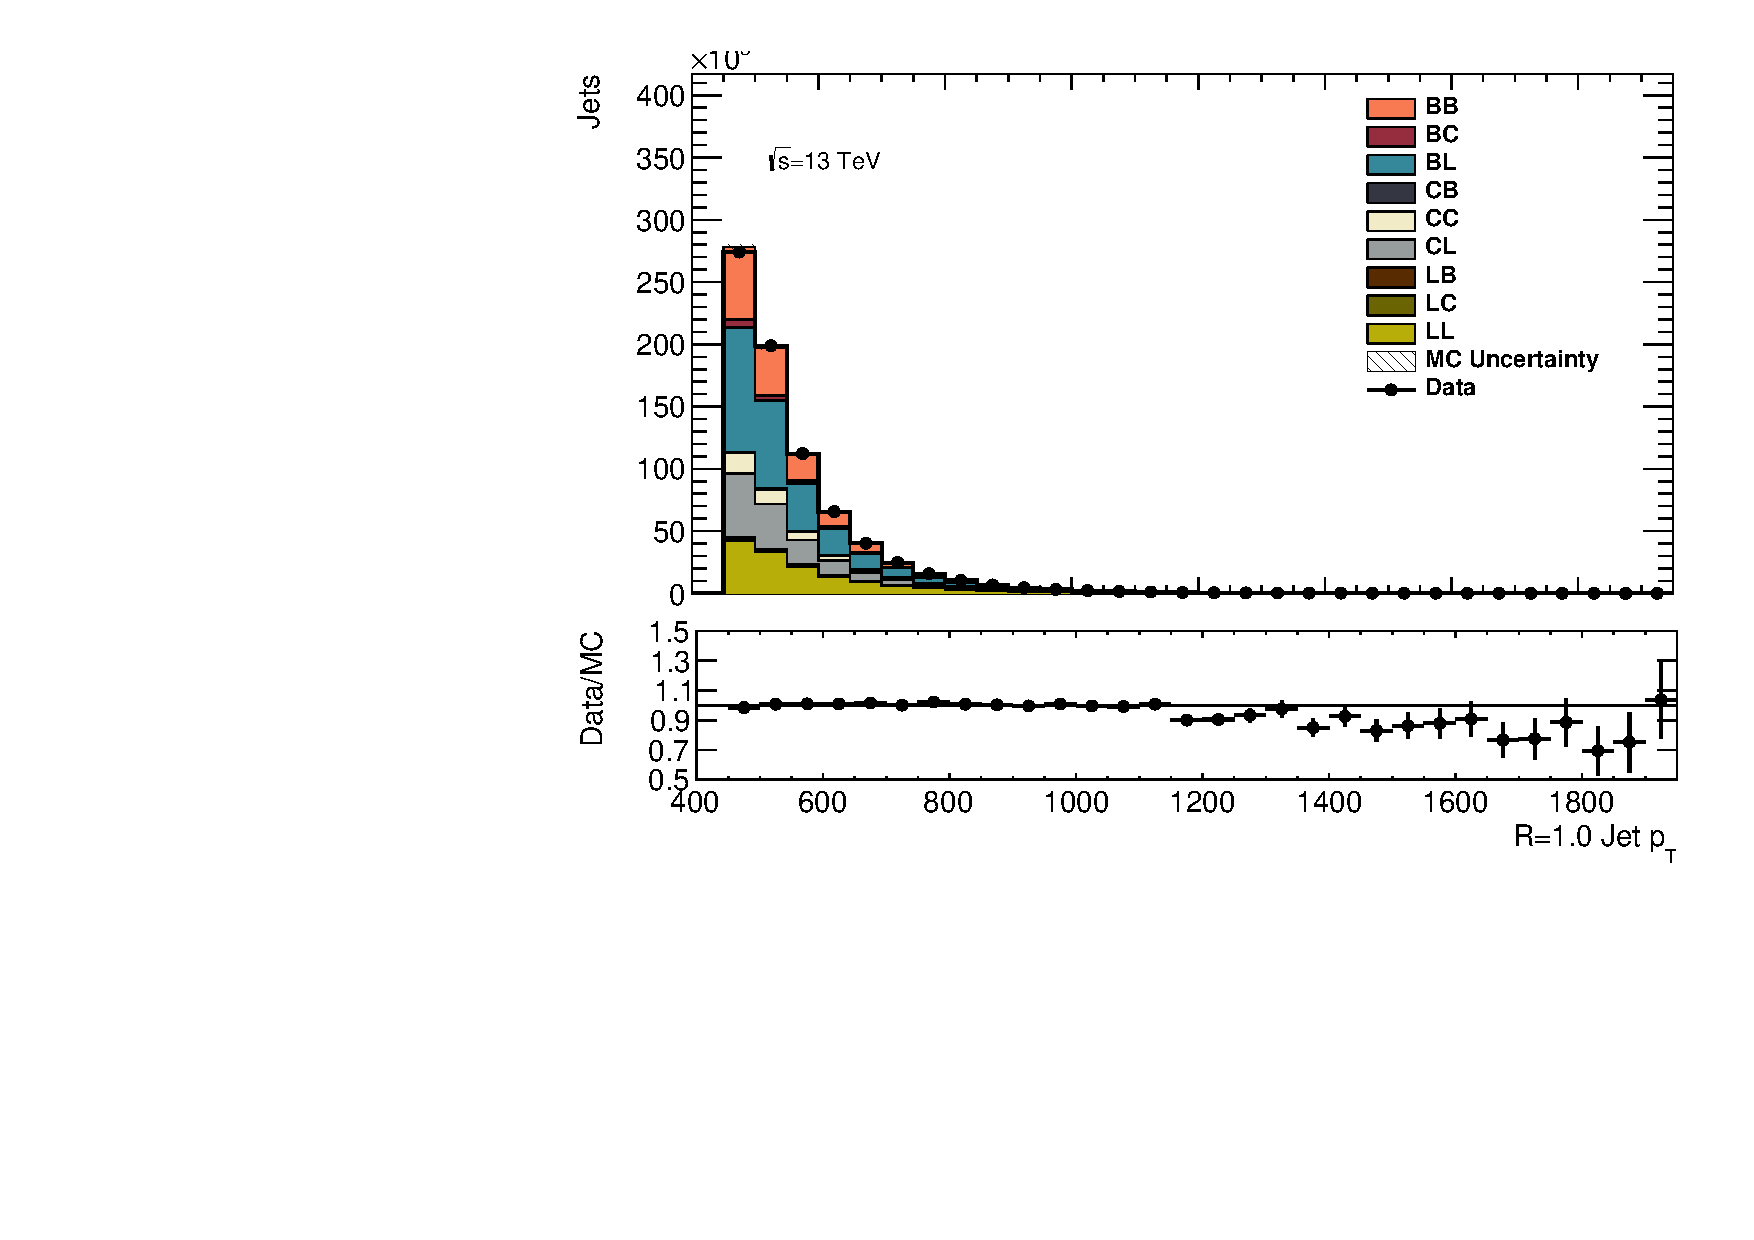
\includegraphics[width=0.38\textwidth]{figures/gbb/LargeRJet_pT_Reweight.pdf}
\caption{Data/MC comparison of $R=1.0$ jet post $b$-tagging without kinematic re-weighting (left) and post $b$-tagging with kinematic re-weighting (right).}% The label of the $R=1.0$ jet flavor content ``XY'' denotes the leading and sub-leading track jet flavor. For example, the flavors of the leading and sub-leading track jet of a ``BL'' $R=1.0$ jet are `B' and `Light' respectively.}
  \label{fig:gbb-pT_largeR}
\end{figure}


\begin{figure}[htbp]
  \centering
  %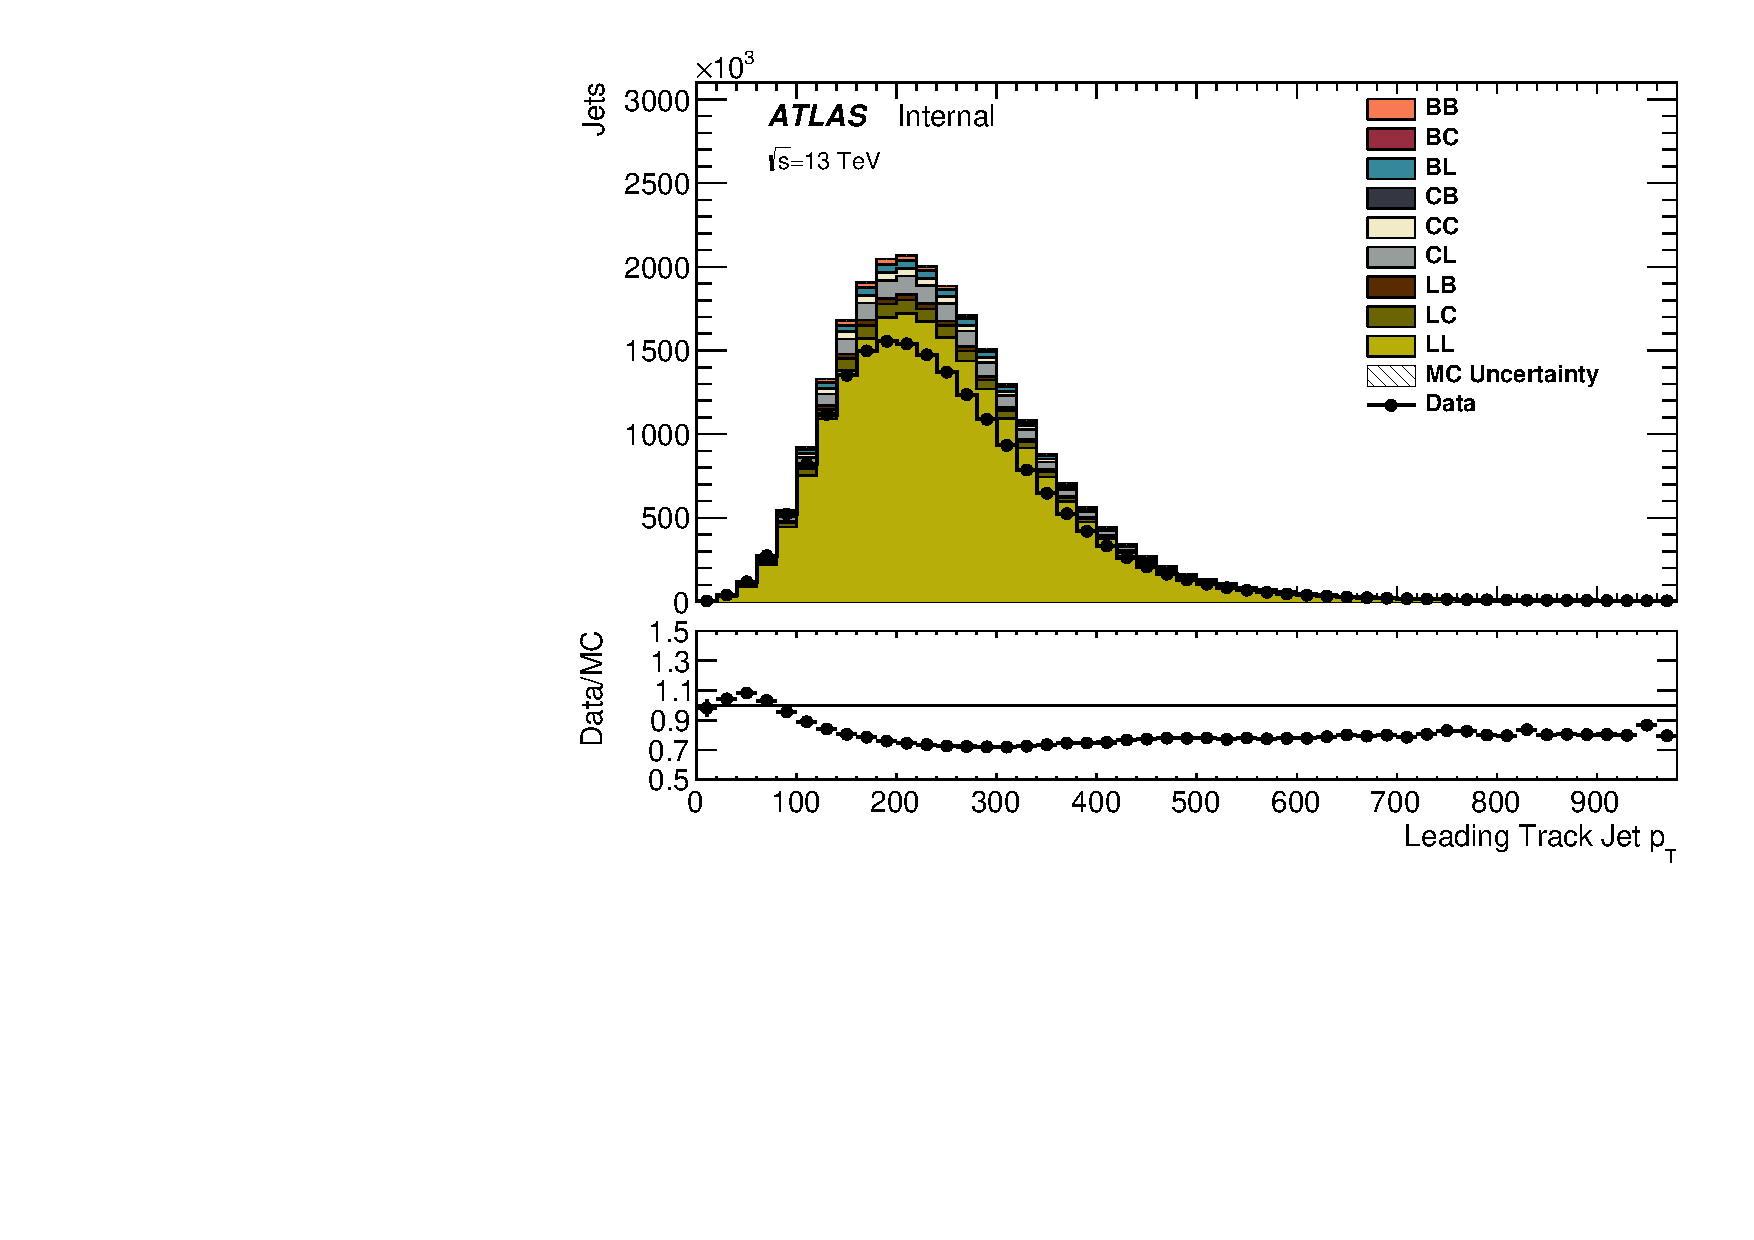
\includegraphics[width=0.38\textwidth]{figures/gbb/LeadTrkJet_pT_NoReweight.pdf}
 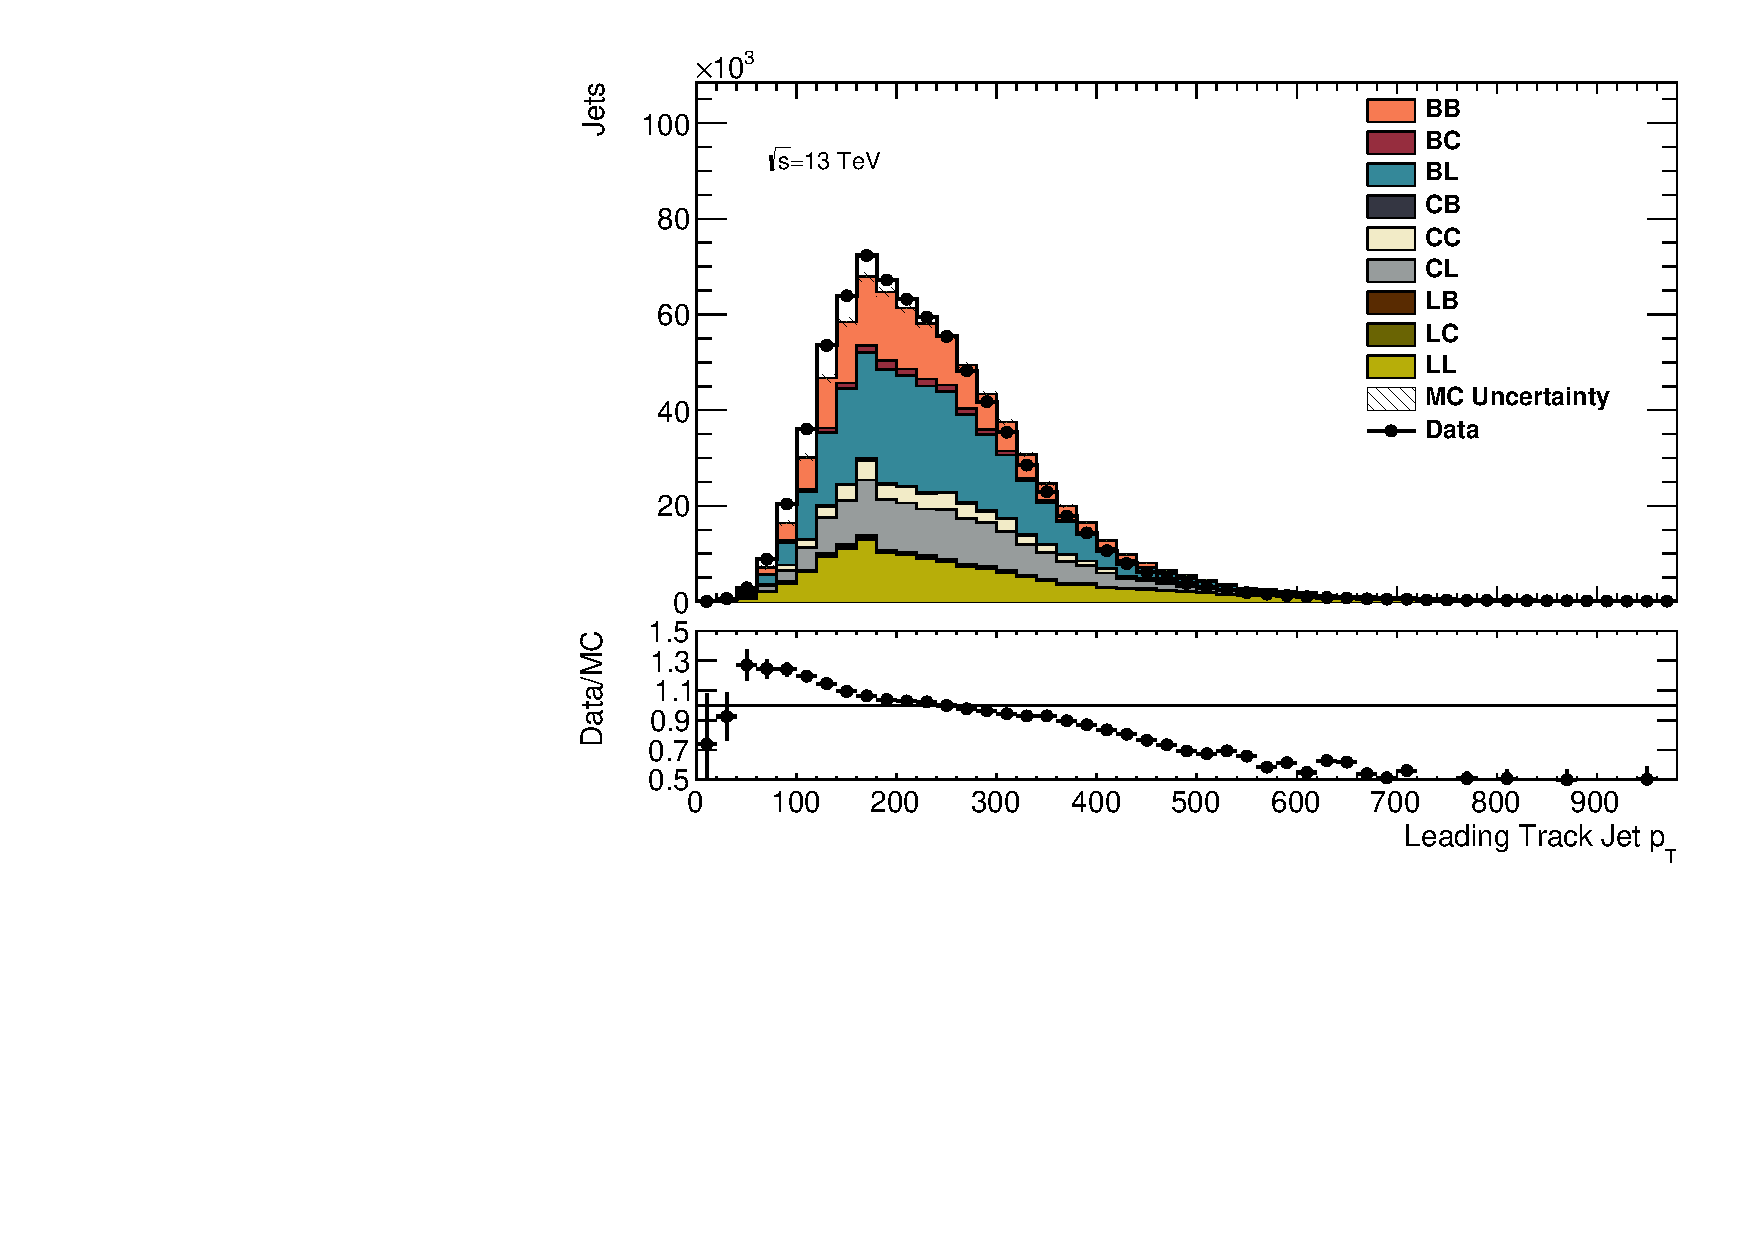
\includegraphics[width=0.38\textwidth]{figures/gbb/LeadTrkJet_pT_PreReweight.pdf}
 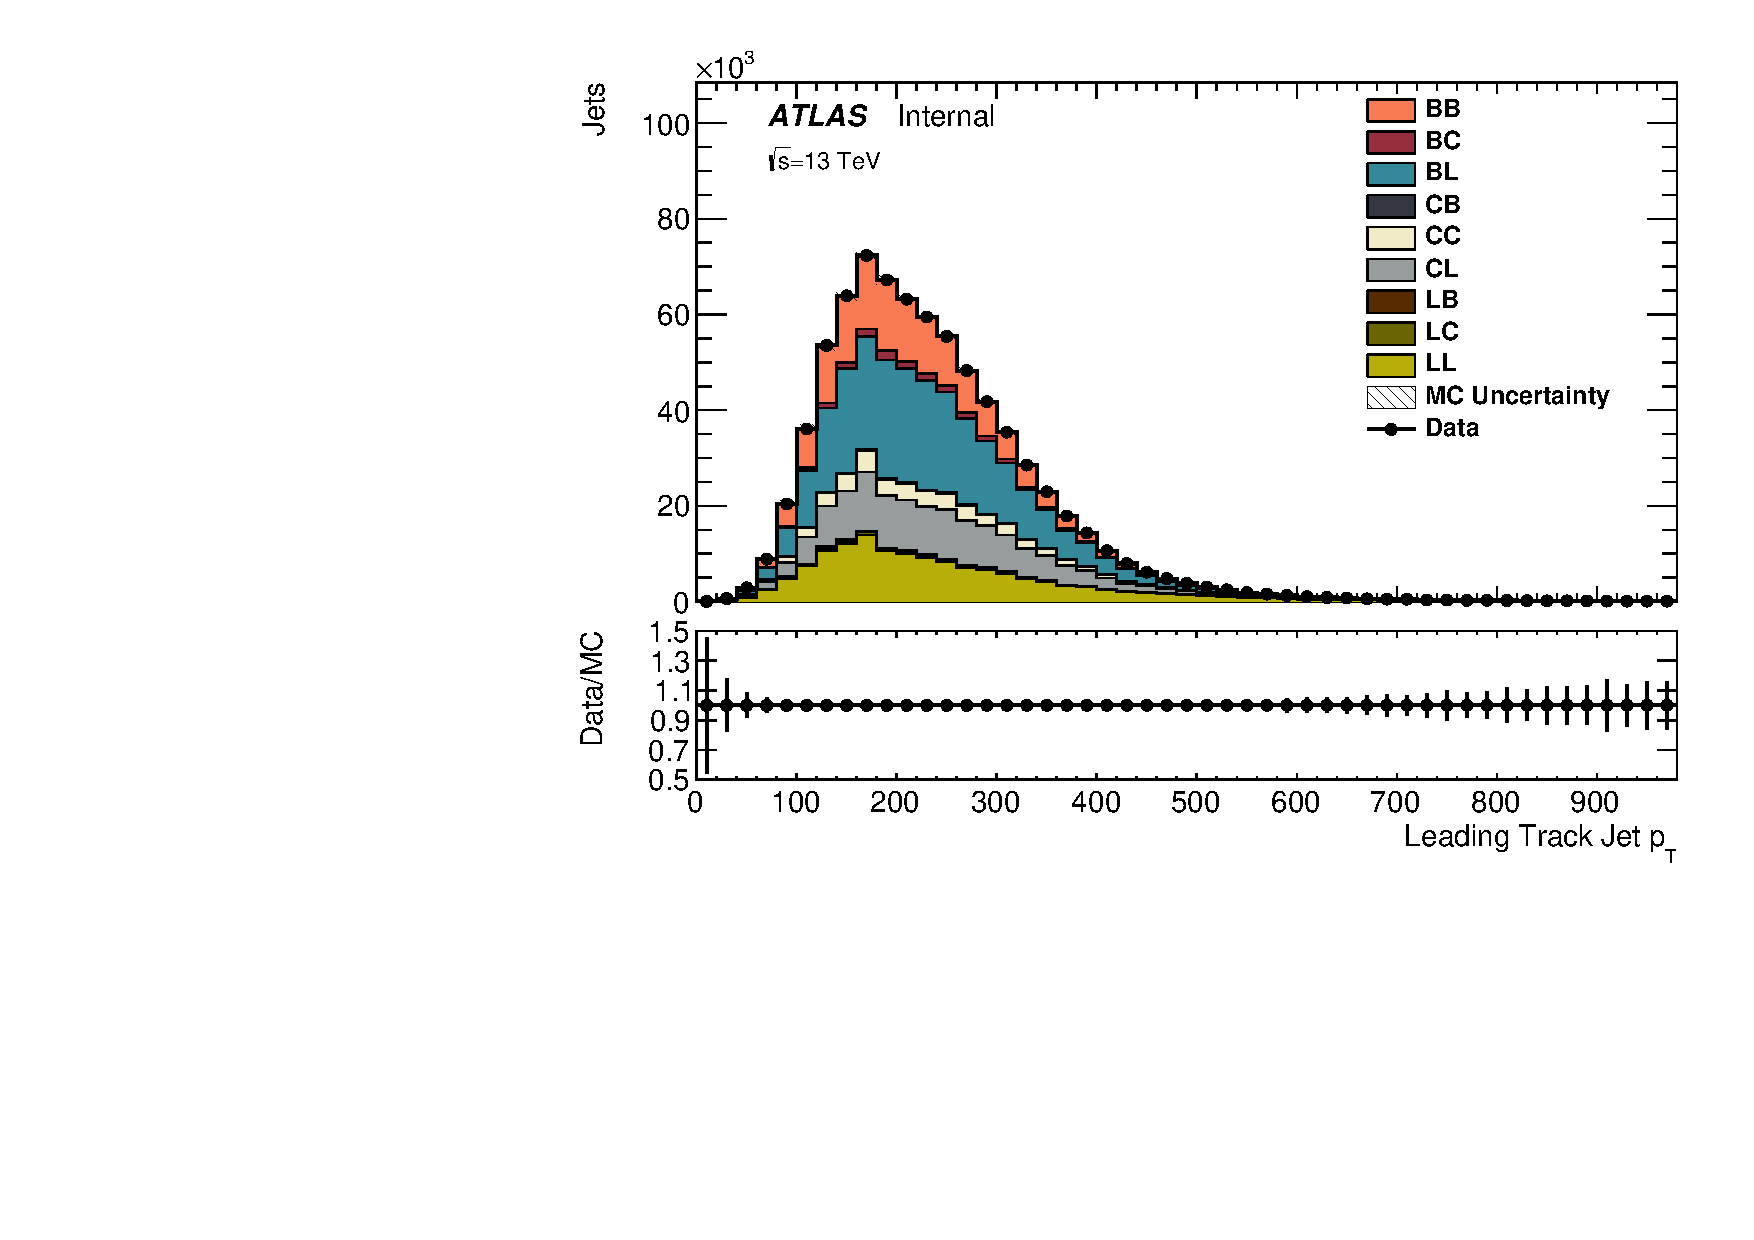
\includegraphics[width=0.38\textwidth]{figures/gbb/LeadTrkJet_pT_Reweight.pdf}
\caption{Data/MC comparison of leading track jets \pt post $b$-tagging without kinematic re-weighting (left) and post $b$-tagging with kinematic re-weighting (right).} % The label of the $R=1.0$ jet flavor content ``XY'' denotes the leading and sub-leading track jet flavor. For example, the flavors of the leading and sub-leading track jet of a ``BL'' $R=1.0$ jet are `B' and `Light' respectively.}
  \label{fig:gbb-pT_leadtrkjets}
\end{figure}


\begin{figure}[htbp]
  \centering
%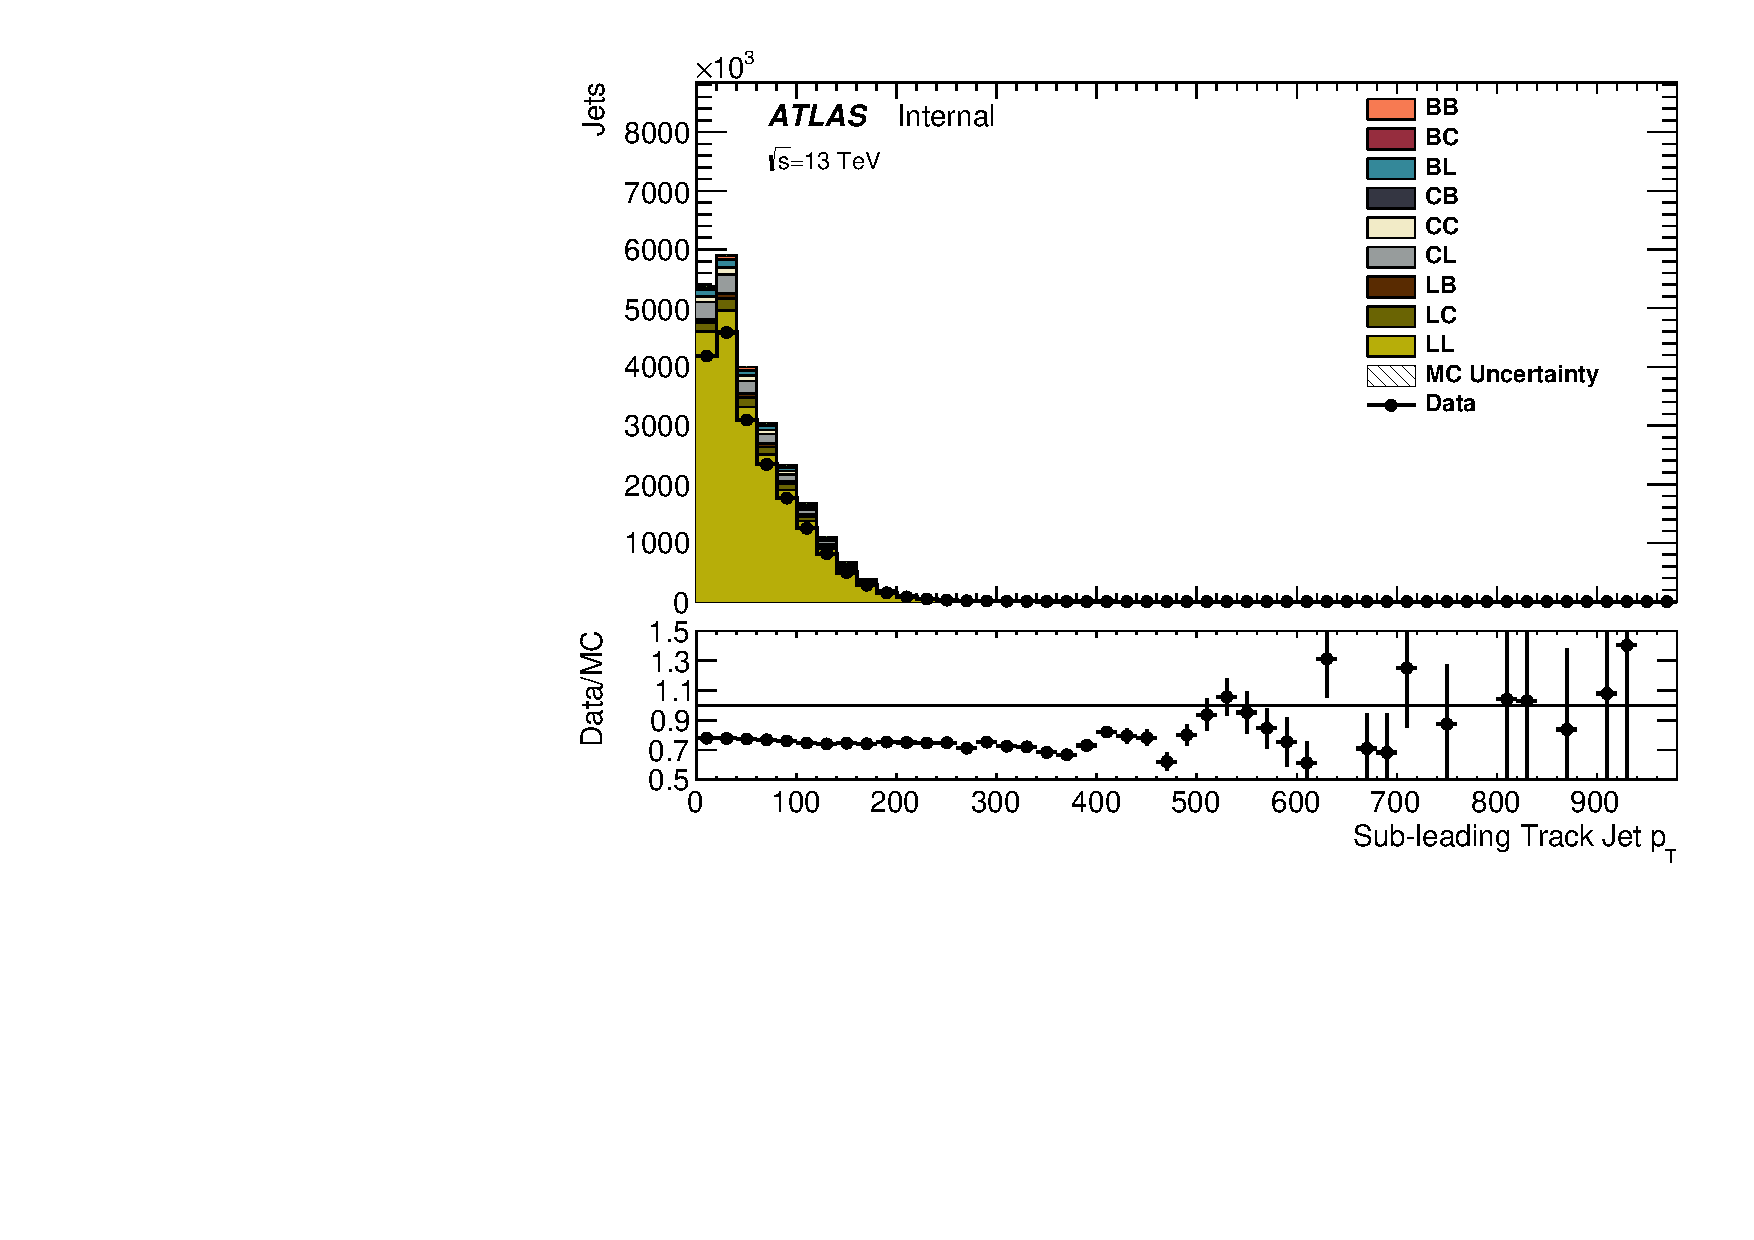
\includegraphics[width=0.38\textwidth]{figures/gbb/SubLeadTrkJet_pT_NoReweight.pdf}
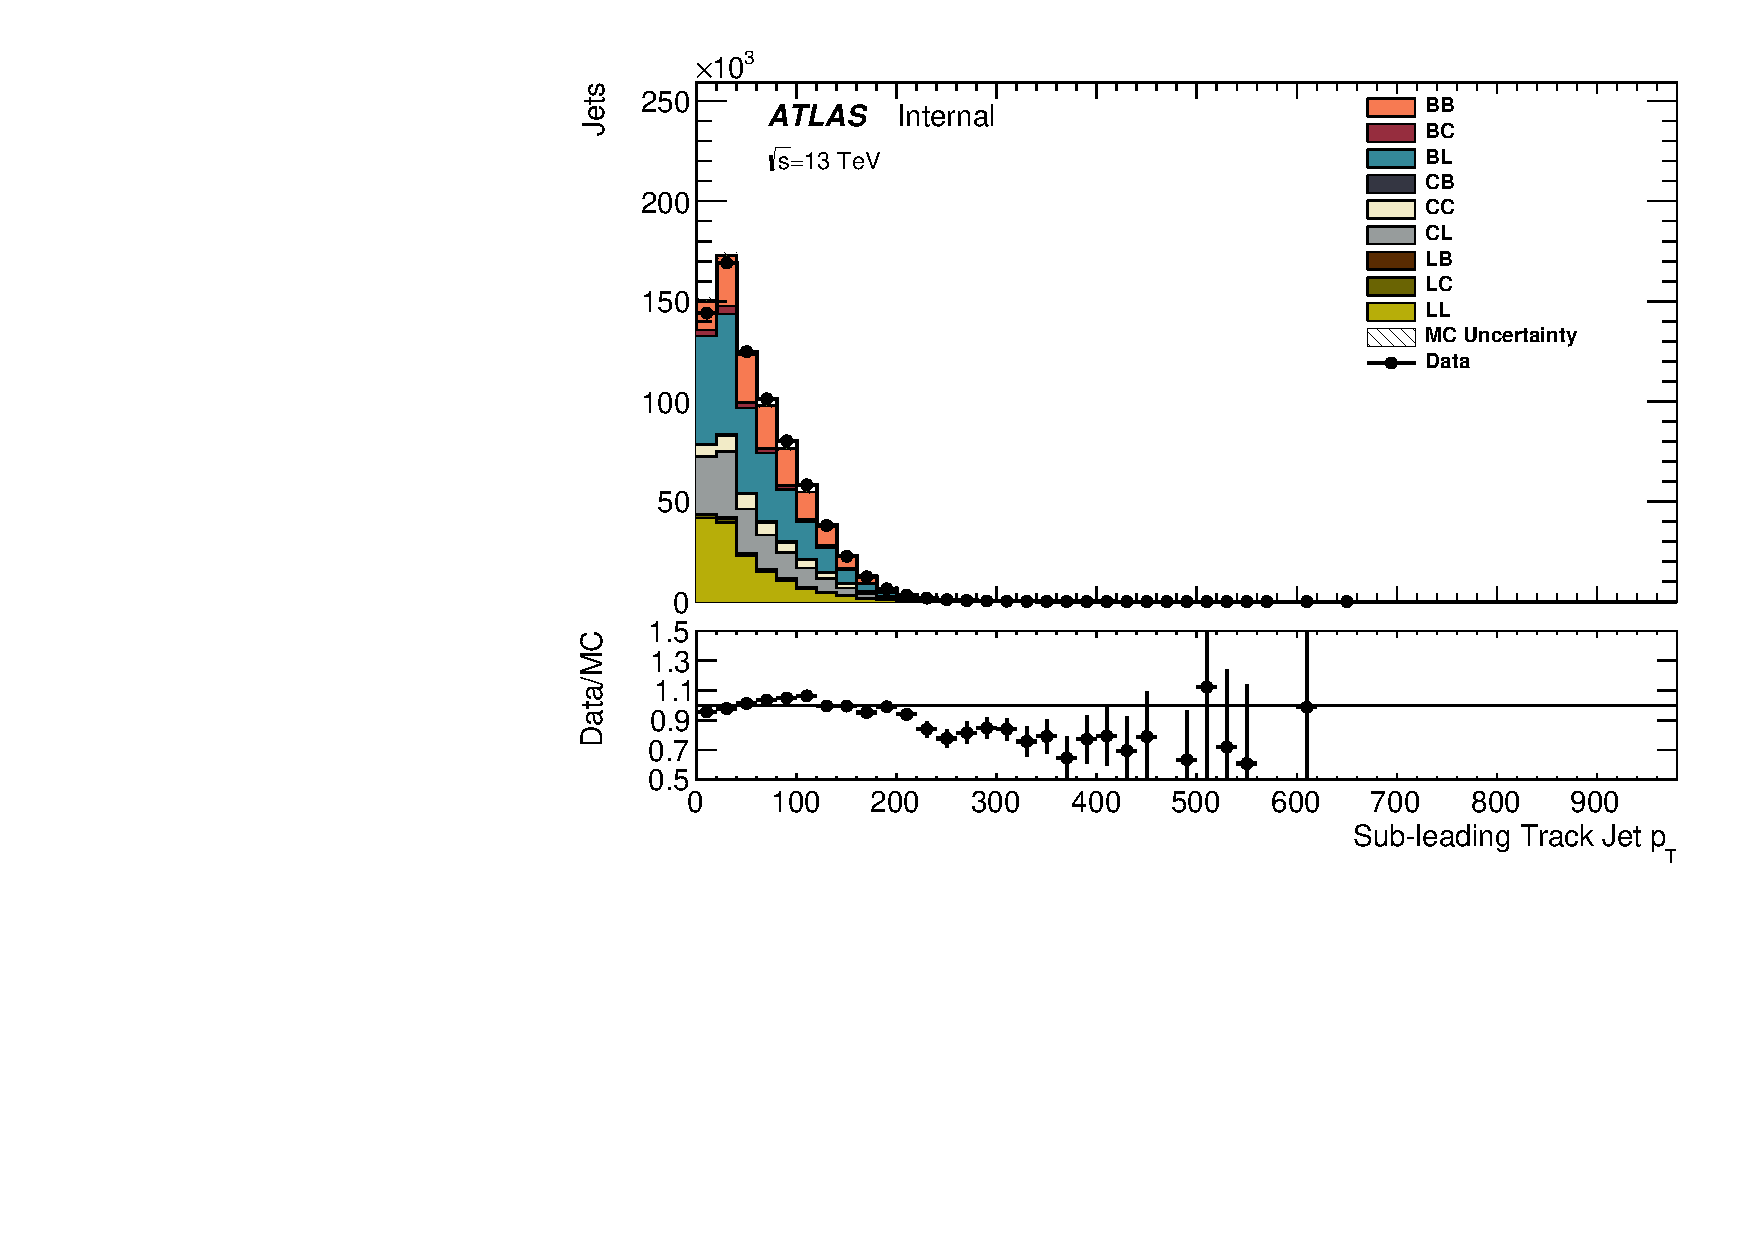
\includegraphics[width=0.38\textwidth]{figures/gbb/SubLeadTrkJet_pT_PreReweight.pdf}
 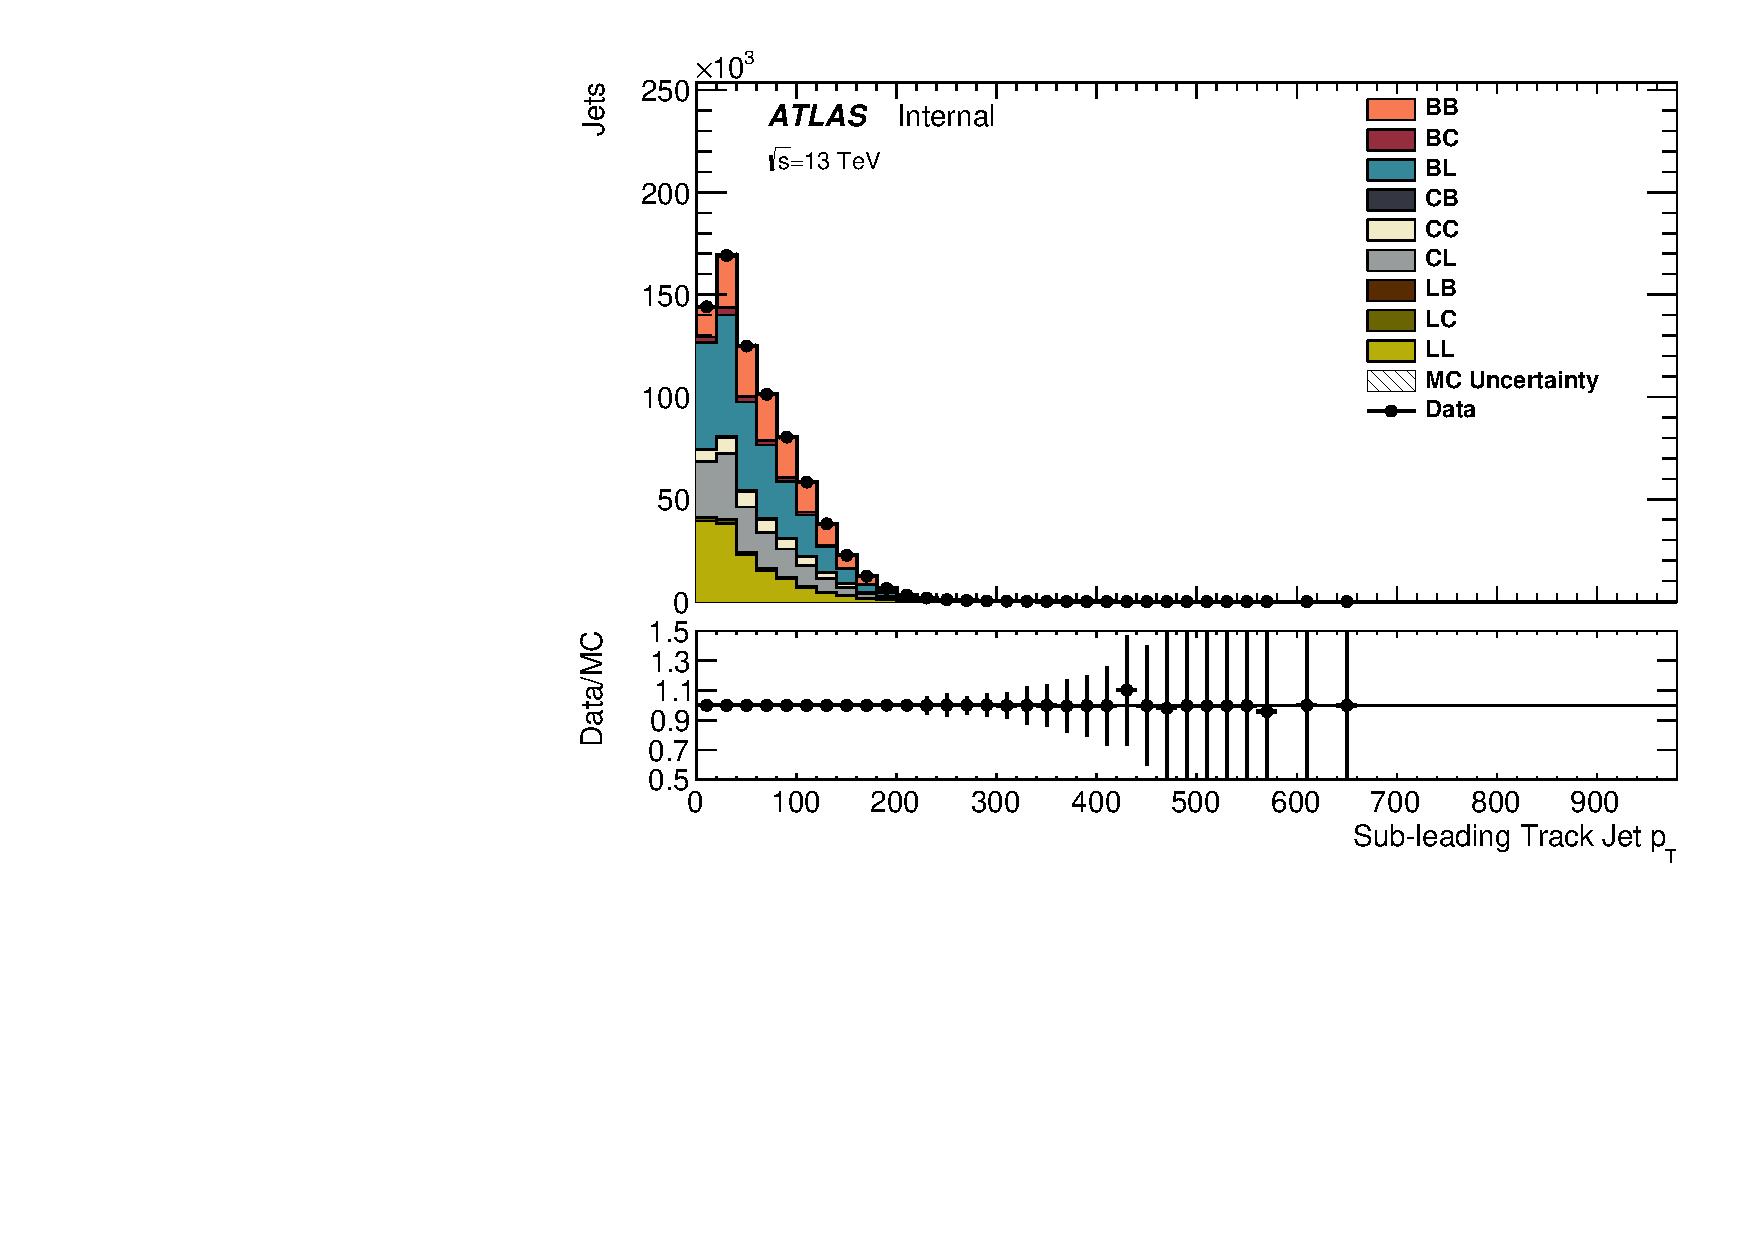
\includegraphics[width=0.38\textwidth]{figures/gbb/SubLeadTrkJet_pT_Reweight.pdf}
\caption{Data/MC comparison of sub-leading track jets \pt post $b$-tagging without kinematic re-weighting (left) and post $b$-tagging with kinematic re-weighting (right).}% The label of the $R=1.0$ jet flavor content ``XY'' denotes the leading and sub-leading track jet flavor. For example, the flavors of the leading and sub-leading track jet of a ``BL'' $R=1.0$ jet are `B' and `Light' respectively.}
  \label{fig:gbb-pT_subtrkjets}
\end{figure}

%-------------------------------------------------------------------------------

%-------------------------------------------------------------------------------
\section{Unfolding}
\label{sec:unfold}
%-------------------------------------------------------------------------------

After subtracting the background from the detector-level distributions, as described in Sec.~\ref{sec:analysis}, the data are corrected for resolution and acceptance effects.  The fiducial volume of the measurement is described by the particle-level object and event selection in Sec.~\ref{sec:obj}.  First, the data are corrected for events that pass the detector-level selection but not the particle-level selection using the simulations introduced in Sec.~\ref{sec:data}.  Then, the iterative Bayes (IB) unfolding technique~\cite{DAgostini:1994zf} is used to correct for the detector resolution in events that pass both the detector-level and particle-level selections.  The IB method is applied with four iterations implemented in the RooUnfold framework~\cite{Adye:2011gm}.  After the application of the response matrix, a final correction is applied to account for events that pass the particle-level but not detector-level selection.  Uncertainties on the unfolding procedure are described in Sec.~\ref{sec:systs}.

%-------------------------------------------------------------------------------
\section{Uncertainties}
\label{sec:systs}
\input{sections/systematics}
%-------------------------------------------------------------------------------

%\clearpage

%-------------------------------------------------------------------------------
\section{Results}
\label{sec:result}
The VBF \Hbb analysis unblinding proceeds in two steps. First, overall strategy is validated with a fit to the $Z$ contribution in a sideband only fit while the Higgs mass window is kept unblinded, shown in Section~\ref{sec:vbf-zunblind}.  Then a simultaneous fit to the signal, correlated over all signal regions, and the $Z$ signal, uncorrelated across signal regions, is done over the entire mass region, as described in~\ref{sec:vbf-higgsunblind}. As an alternative interpretation of this analysis the $\mu_{VBF}$ strength is extracted by only allowing $VBF$ events to float in the fit and fixing all other Higgs processes, i.e. ggF, ttH and VH, to Standard Model expectation, as described in~\ref{sec:vbf-higgsunblindvbf}. The combination of inclusive $VBF$ and $VBF+\gamma$ results are presented in~\ref{sec:vbf-higgscomb}.


\subsection{Unblinding of \zjets{} in mass sidebands}
\label{sec:vbf-zunblind}

The fit strategy is first validated in data with a closure obtained in \zjets{} mass sideband fit. We performed a side-band only fit to extract the \zjets{} contribution independently in all regions. The fitted \zjets{} strengths are summarized in Table~\ref{tab:zsidebandfit}, presented with with all experimental and statistical uncertainties.   Note that we have no BDT shape uncertainties on the \zjets{} MC so cannot draw any conclusions from the compatibility of $\mu_Z$ with 1 in the different BDT regions. The effective $\mu_{Z}^{\rm eff}$ of all regions combined is defined as
\begin{equation}
\label{eqn:zsig}
\mu_{Z}^{\rm eff} = \sum \mu_{Z,i}\frac{n_{Z,i}}{\sum n_{Z,i}} 
\end{equation}
where $n_{Z,i}$ is the number of $Z$ events in region $i$, and $\mu_{Z,i}$ is the measured $\mu_Z$ in region $i$.  $\mu_{Z}^{\rm eff}$ is measured to be $1.0\pm 0.4$ in the sideband only fit with a compatibility of $\chi^2/nodf = 5.5/6=0.9$ ($\chi^2$ probability of 48\%).


\begin{table}[htbp]
\centering
\caption{Floating Z normalization parameters in data sideband fit including all systematic uncertainties.}
\label{tab:zsidebandfit}
\begin{tabular}{|l|c|c|}
\hline
Channel      & $\mu_{Z}$   & $\chi^2/ndof$ \\ \hline
2 cen SR I   & 2.6 $\pm$1.3  & 1.1          \\ \hline
2 cen SR II  & 0.4$\pm$0.8  & 0.7          \\ \hline
4 cen SR I   & 2.2$\pm$2.0  & 0.8          \\ \hline
4 cen SR II  & 2.0$\pm$1.9  & 0.9          \\ \hline
4 cen SR III & 1.9$\pm$0.6  & 0.9          \\ \hline
4 cen SR IV  & 0.6$\pm$0.6  & 0.9          \\ \hline
\end{tabular}
\end{table}



%\begin{figure}[htbp]
%  \centering
% 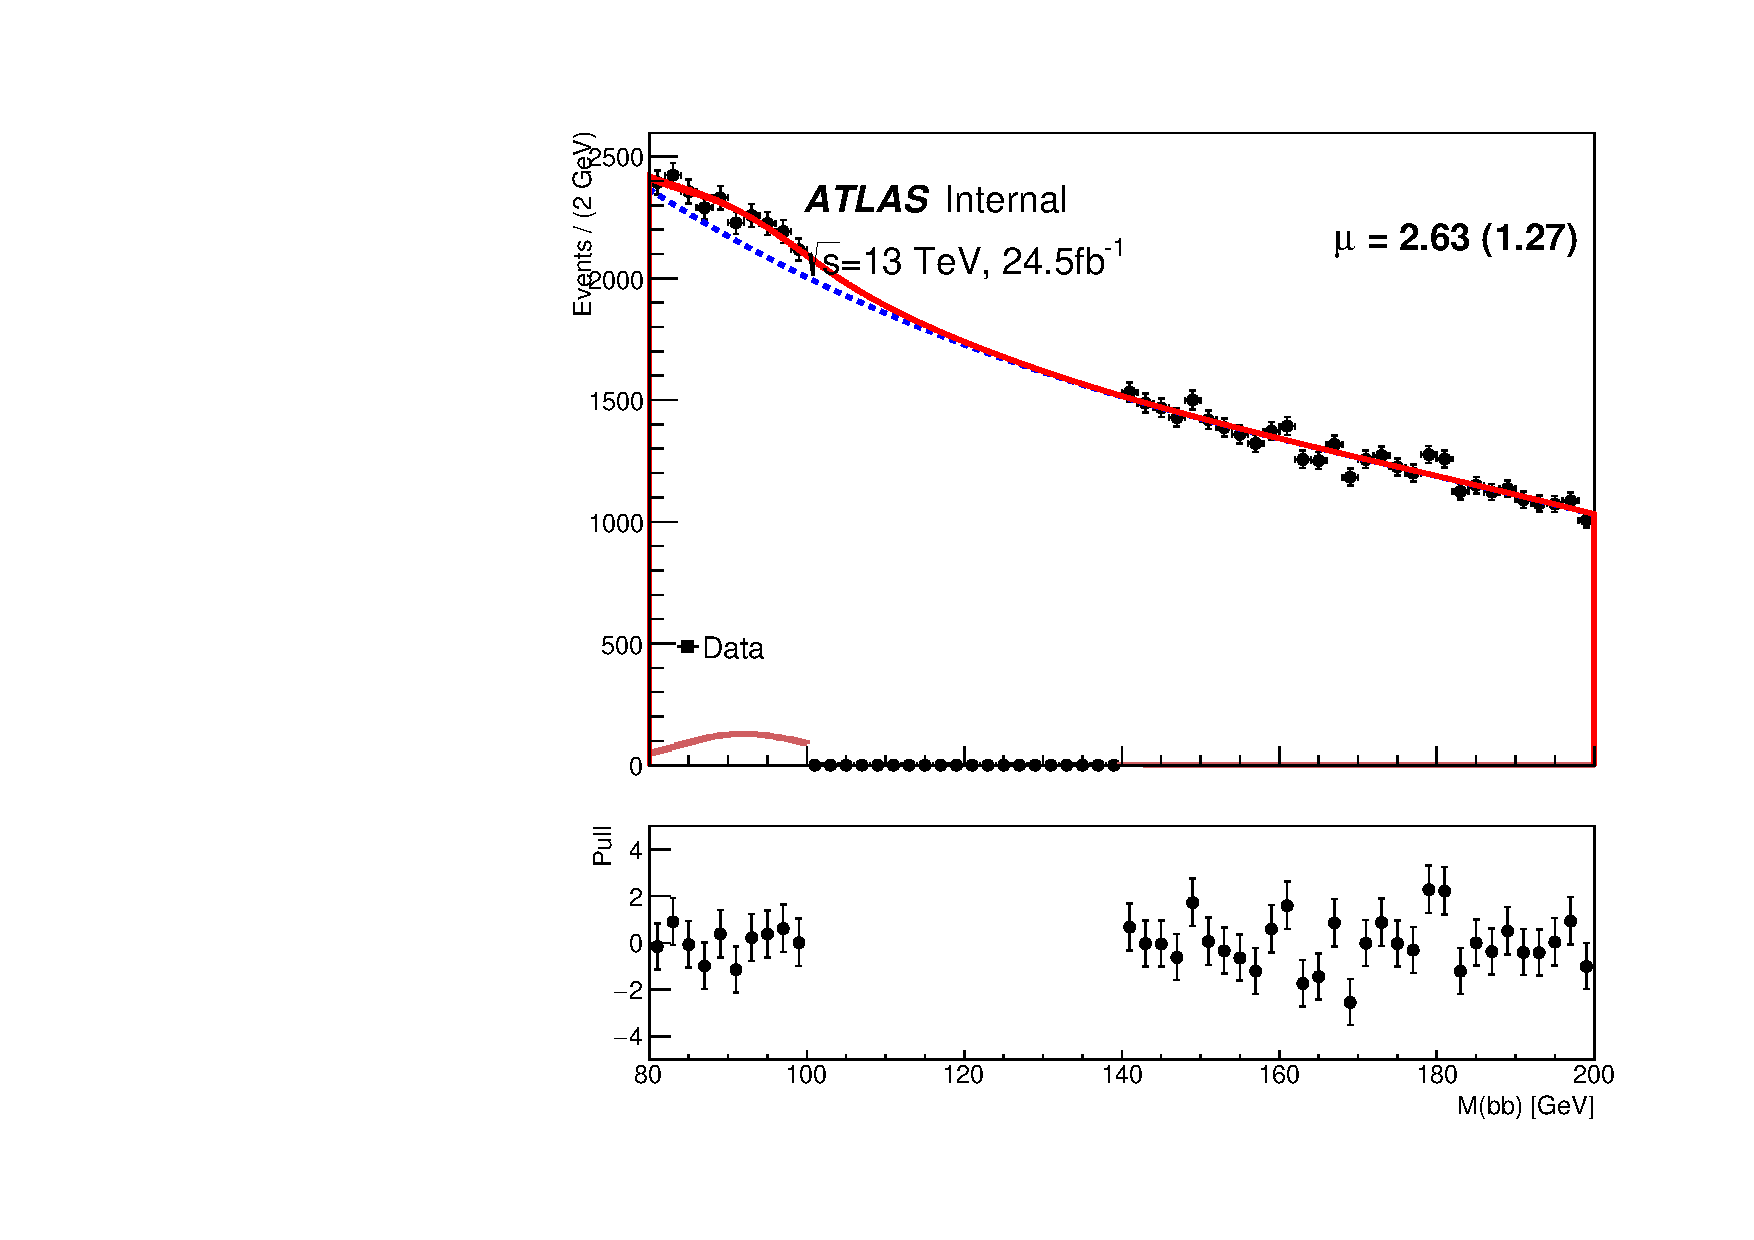
\includegraphics[width=0.24\textwidth]{figures/VBF/zunblind_testVBF_ICHEP_2cen_SRI.pdf}
% 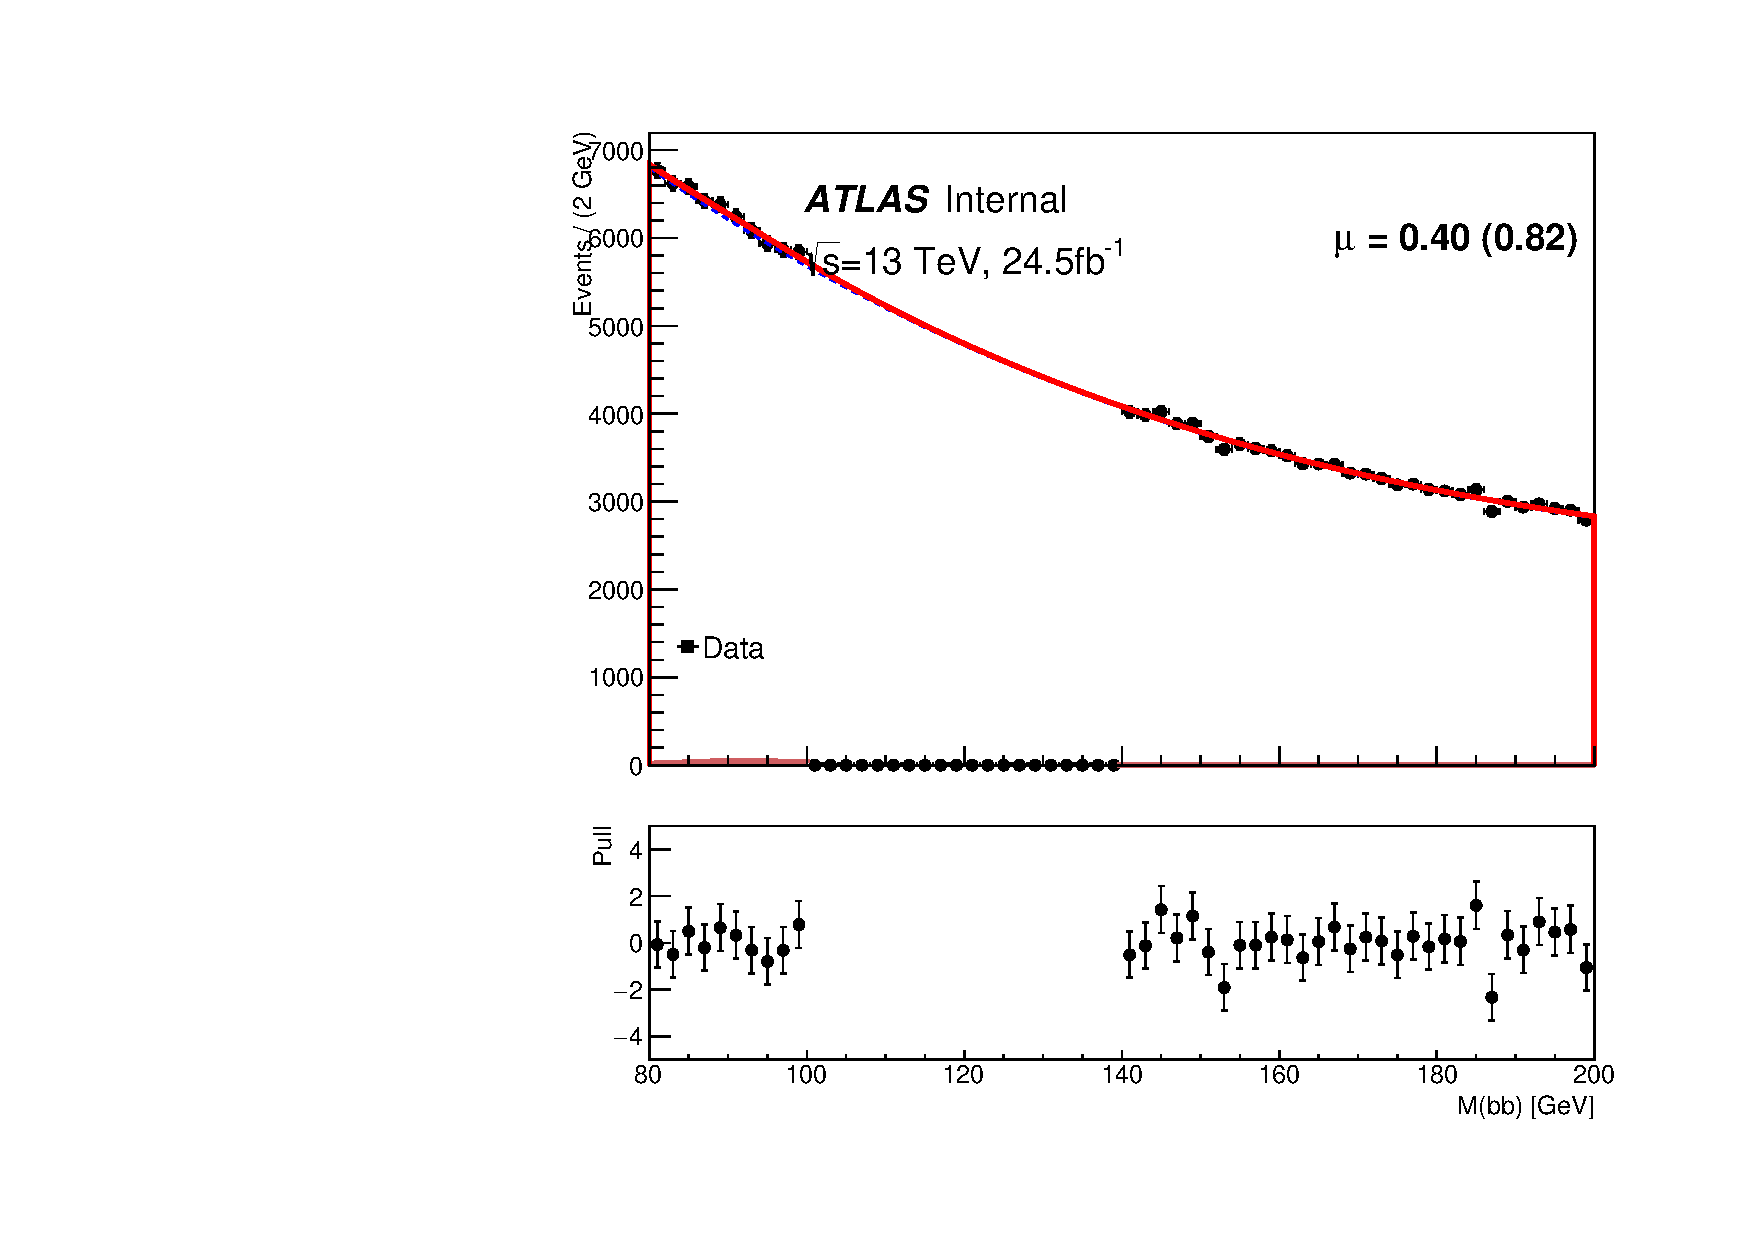
\includegraphics[width=0.24\textwidth]{figures/VBF/zunblind_testVBF_ICHEP_2cen_SRII.pdf}\\
% 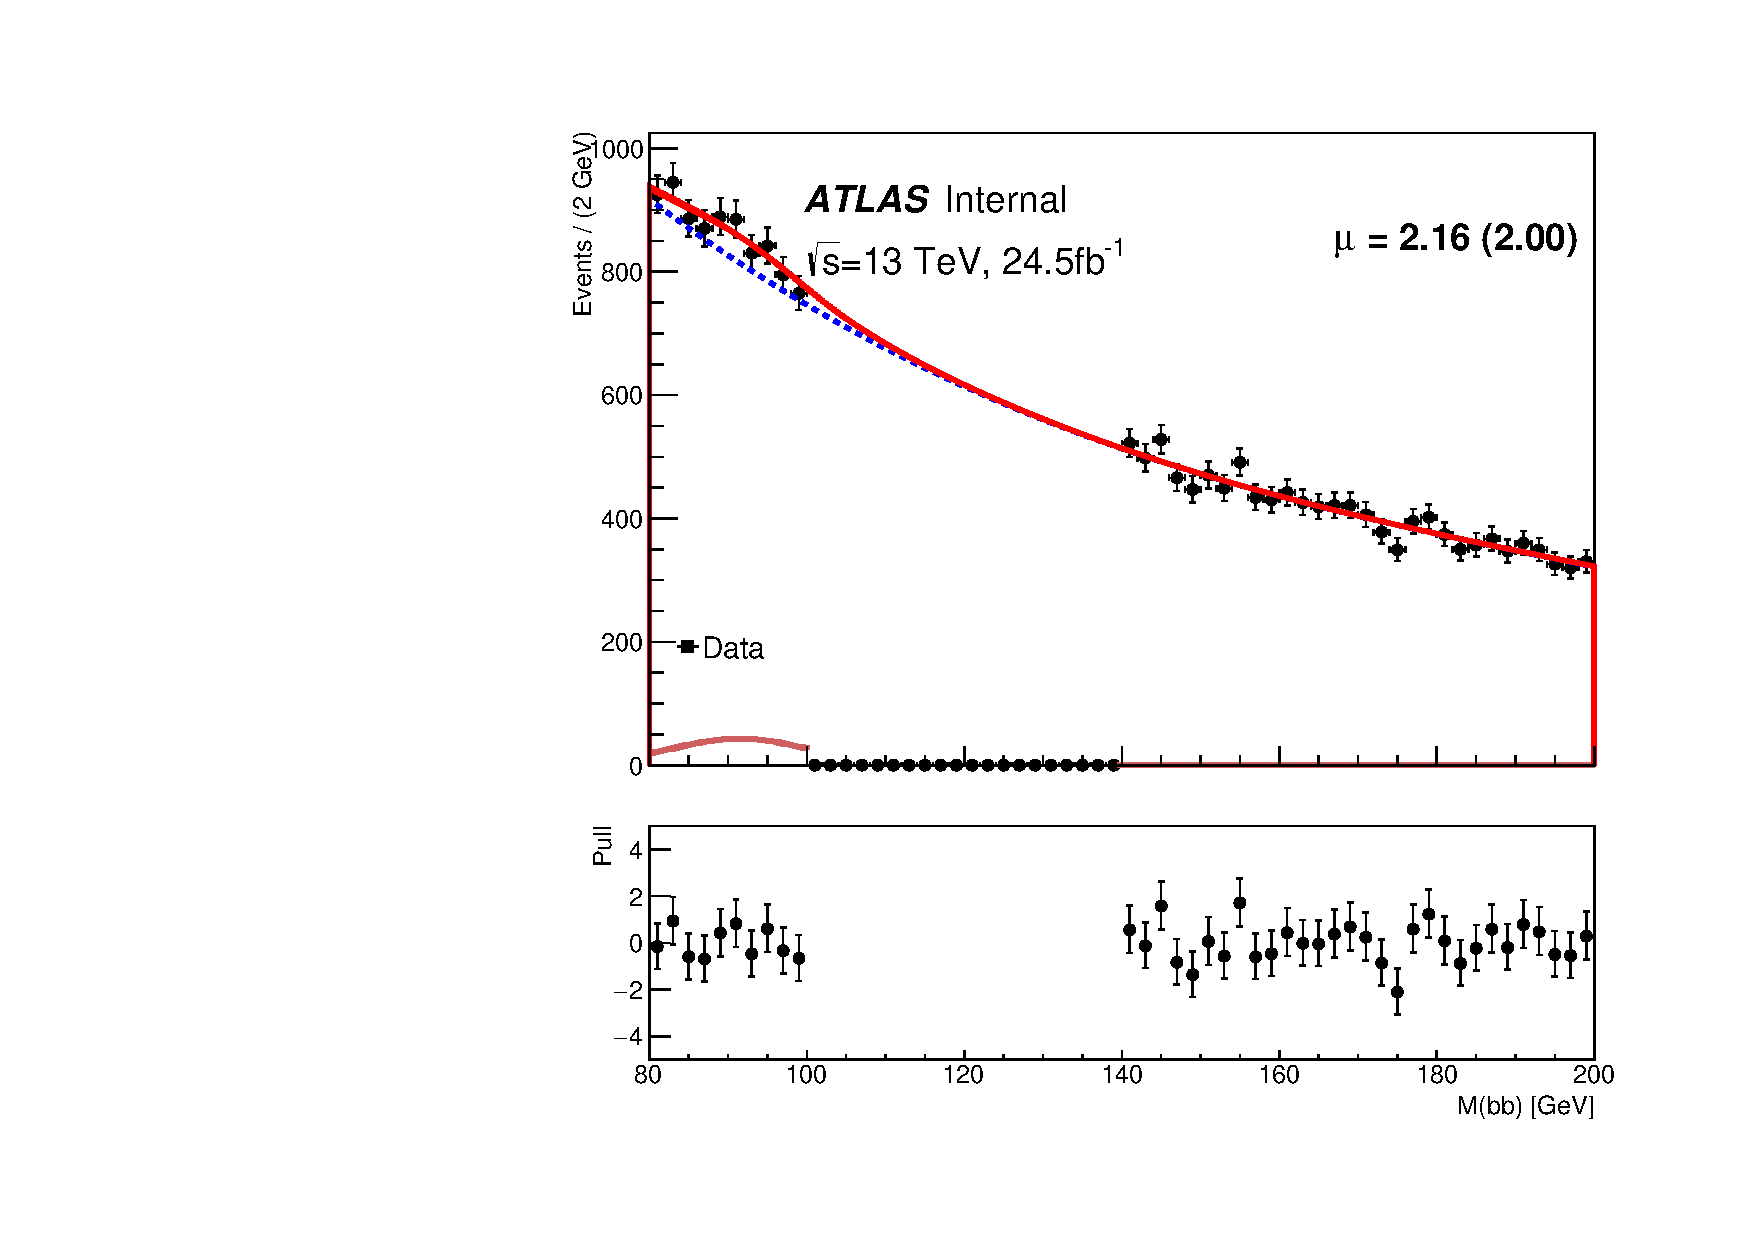
\includegraphics[width=0.24\textwidth]{figures/VBF/zunblind_testVBF_ICHEP_4cen_SRI.pdf}
% 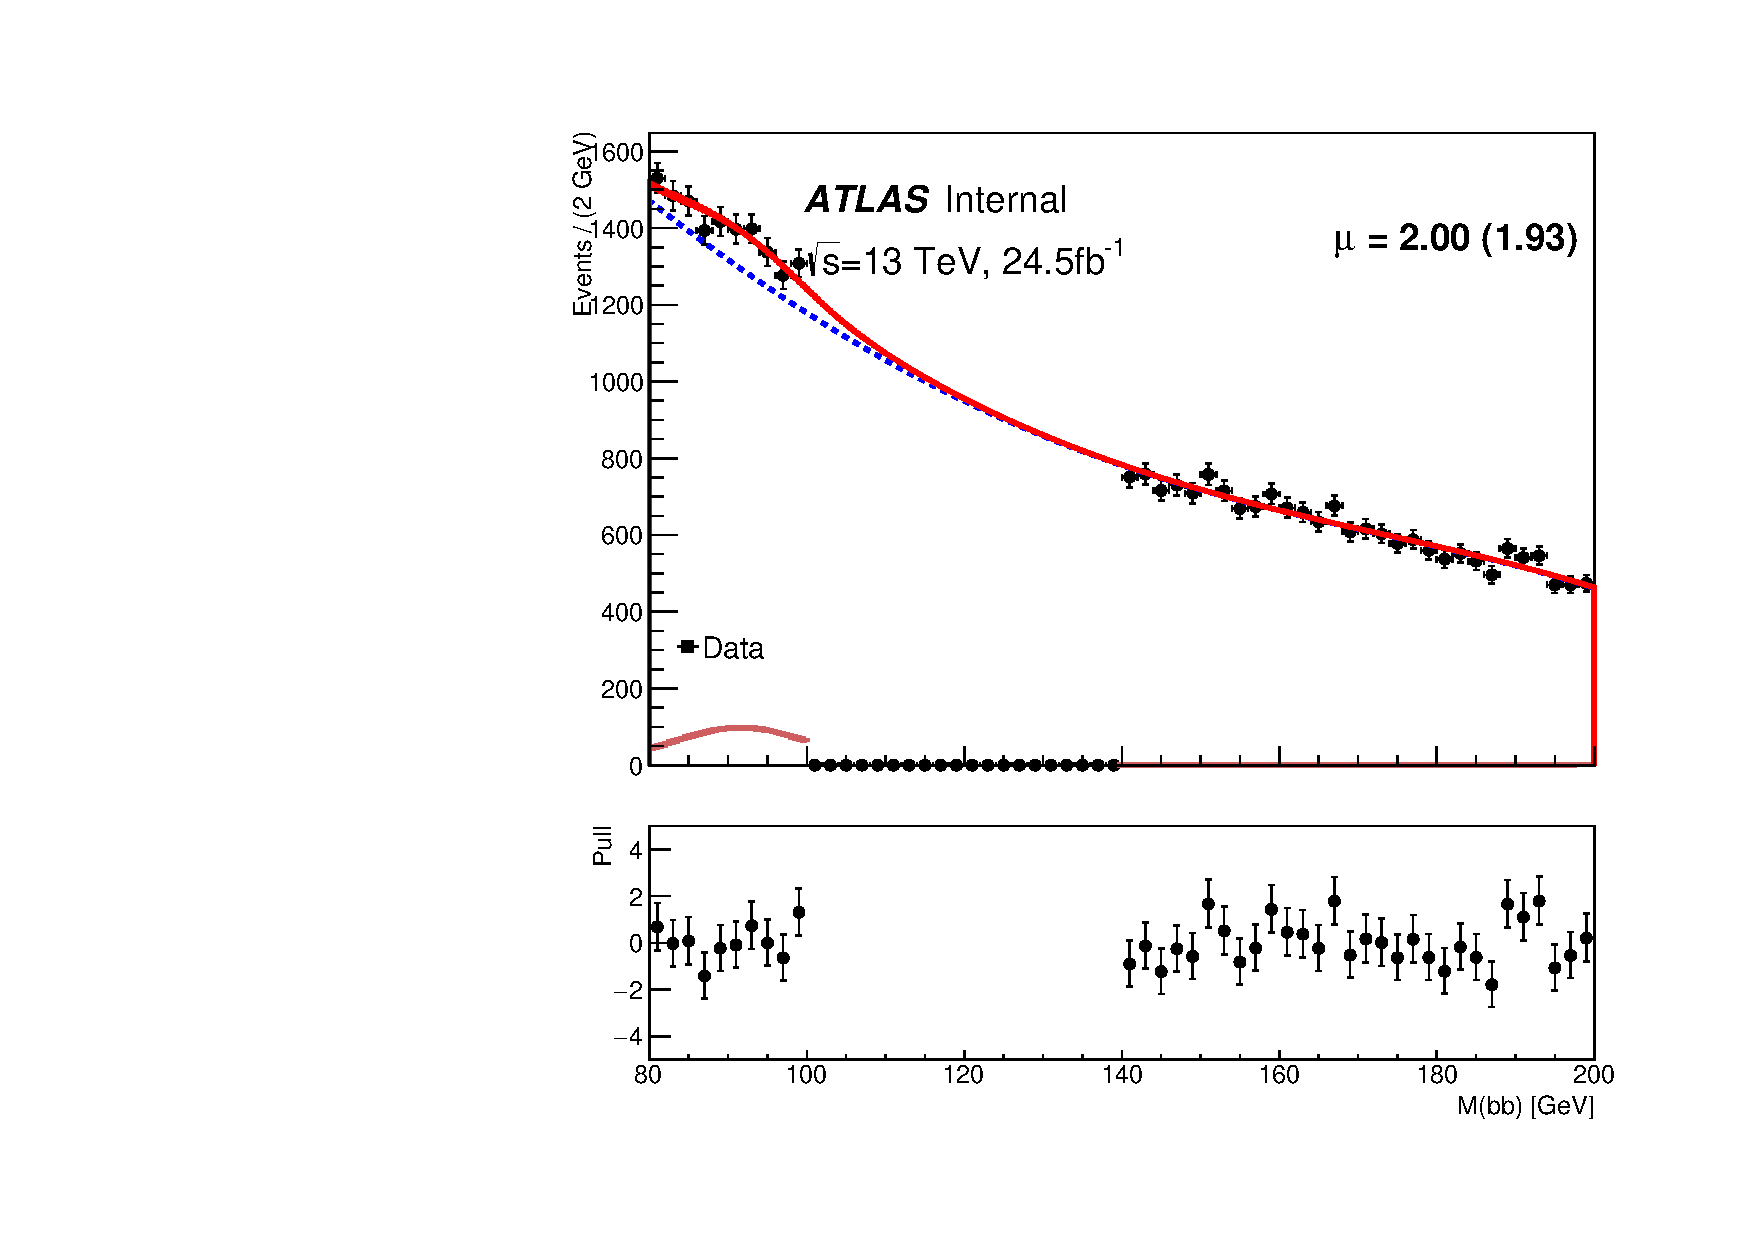
\includegraphics[width=0.24\textwidth]{figures/VBF/zunblind_testVBF_ICHEP_4cen_SRII.pdf}
% 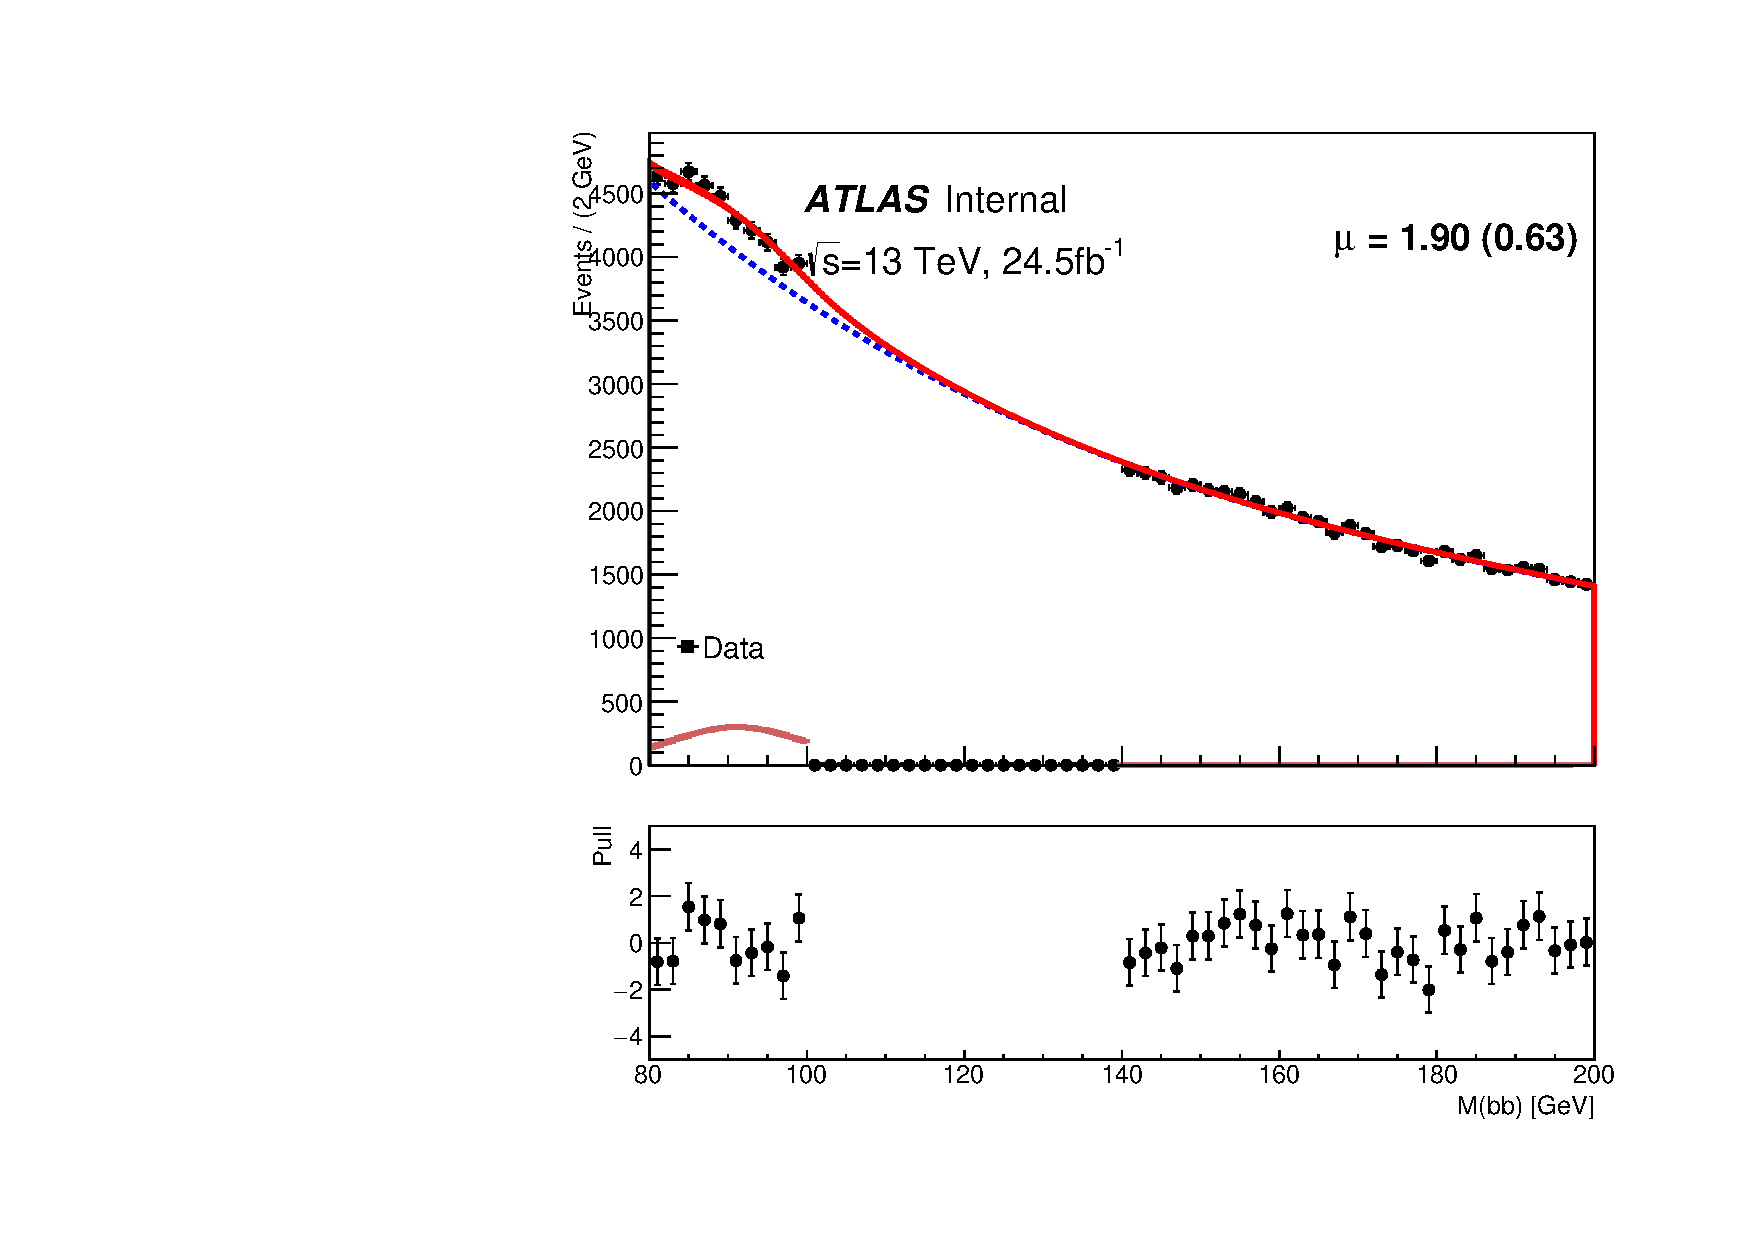
\includegraphics[width=0.24\textwidth]{figures/VBF/zunblind_testVBF_ICHEP_4cen_SRIII.pdf}
% 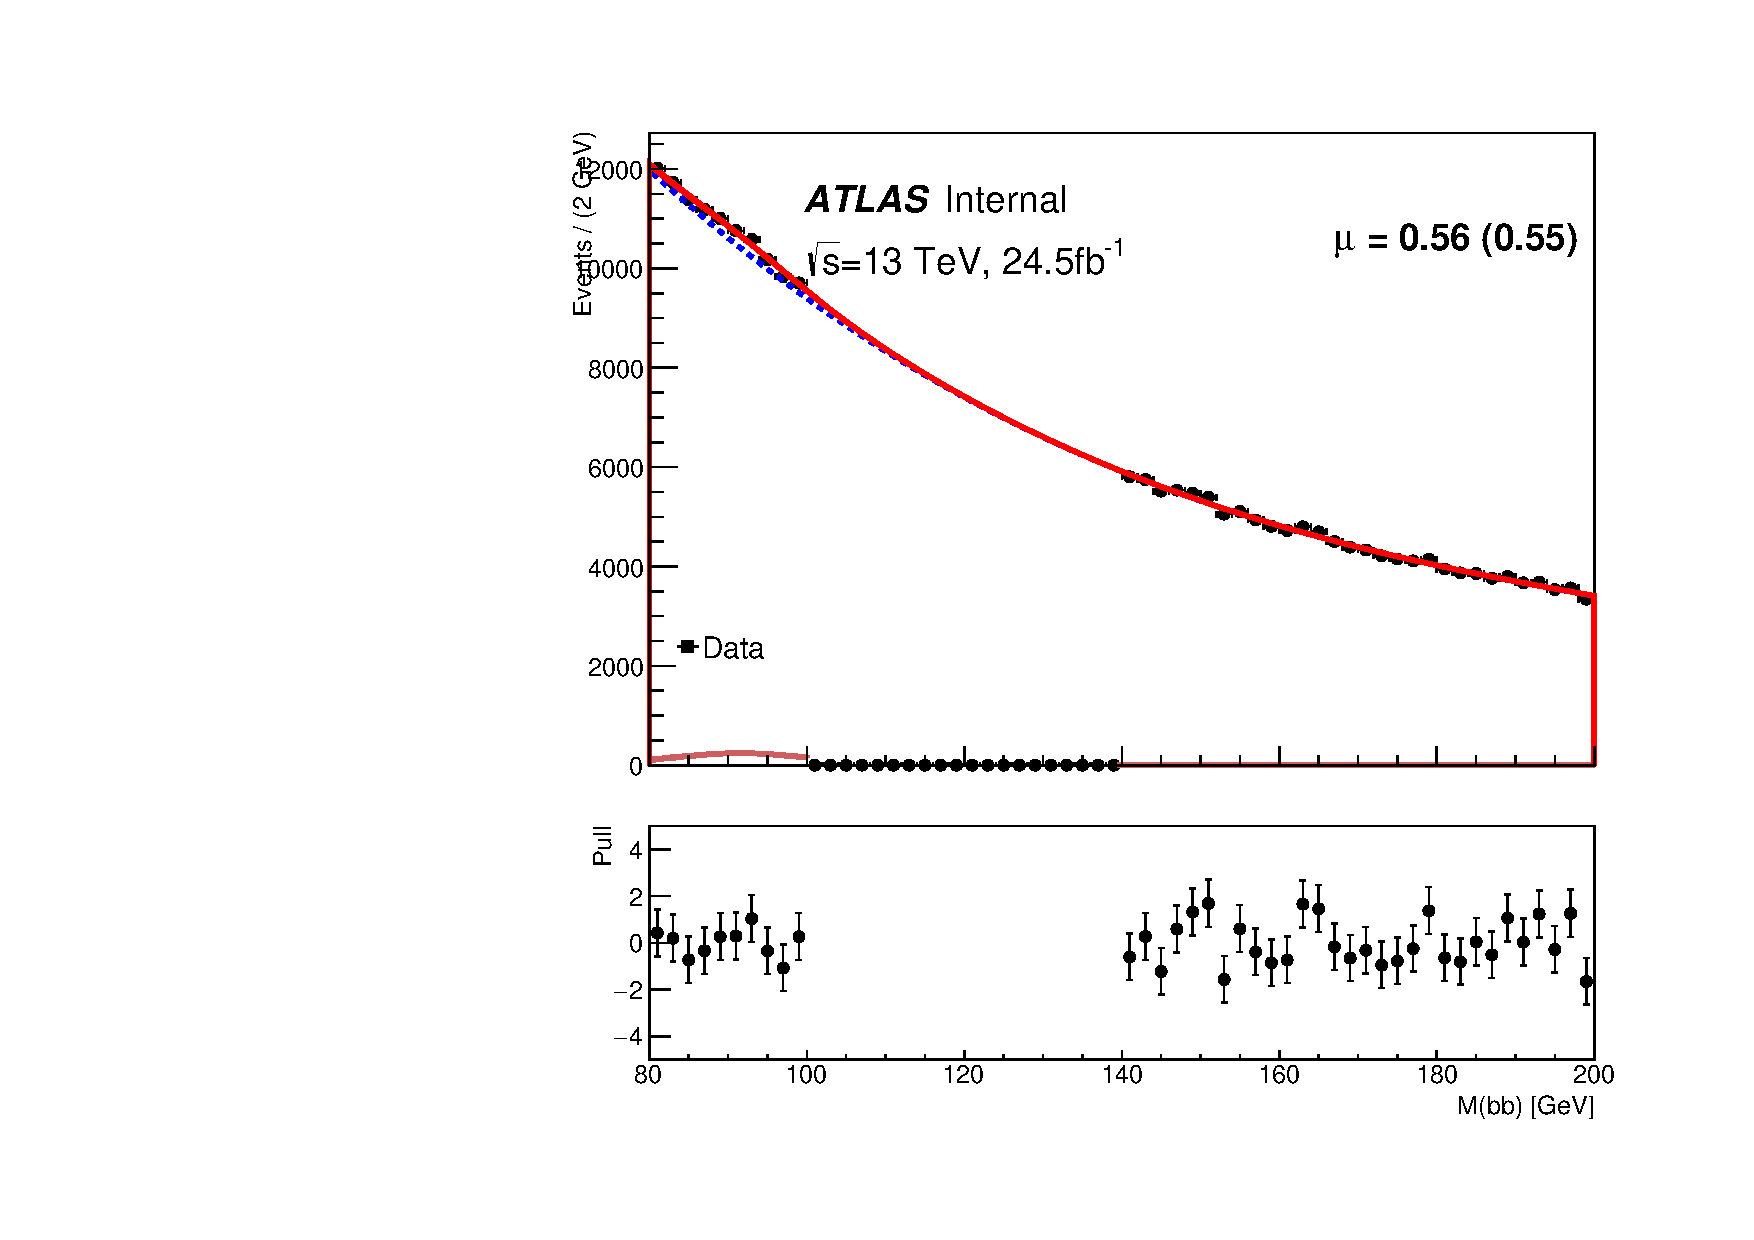
\includegraphics[width=0.24\textwidth]{figures/VBF/zunblind_testVBF_ICHEP_4cen_SRIV.pdf}\\
%\caption{Data and fit model comparison for sideband only \zjets{} fit in \twocentral (top) and \fourcentral channel (bottom) for SR I (left) to SR IV (right).  The data are the black points and the fit model (red), which comprises the continuum background (blue dashed line) and the Z contribution (light red histogram).}
%  \label{fig:vbf-zsidebandfit}
%\end{figure}


\subsection{Extraction of $\mu_{H}$}
\label{sec:vbf-higgsunblind}

The observed value of the Higgs signal strength is $2.7^{+2.2}_{-2.0}$, while the Asimov fit yields $\mu_{H}=1\pm 1.9$. The breakdown of the uncertainty is $\mu_H=2.7^{+1.9}_{-1.9}\textnormal{(stat)}^{+1.1}_{-0.6}\textnormal{(syst)}$ treating the NPs for the analytical background parameterization and normalization as well as the normalization of $Z$ contribution as statistical uncertainty.

%Figures~\ref{fig:vbf-higgsfit_2cen} and ~\ref{fig:vbf-higgsfit_4cen} show the resulting distributions for the \twocentral and \fourcentral channels. %displaying the residuals with respect to the continuum background fit on the bottom panel. % whereas Figures~\ref{fig:vbf-higgsfit_2cen_pull} and~\ref{fig:vbf-higgsfit_4cen_pull} show the pull values with respect to the full background model.  

%The pull values are shown in Figure~\ref{fig:vbf-higgsfitpull} for nuisance parameters with a post-fit impact of more than 4\%.  None of the nuisance parameters are strongly pulled. The largest uncertainty on $\mu_H$ comes from the theory uncertainty on the QCD scale, followed by the background parameterization and the jet energy resolution. The increase of the total uncertainty with respect to the expected value comes from the larger than expected background normalization as well as an increase of the signal systematics which scales as the size of the $\mu_H$. 

The fitted $Z$ values are shown in Table~\ref{tab:zfullfit} for each SR.  Reductions of 30--60\% of the $\mu_Z$ uncertainties are observed with respect to the sideband only fit. A statistical combination of all the channels, as described in Equation~\ref{eqn:zsig}, yields an effective $\mu_Z = 1.2 \pm 0.2$ with a combined $\chi^2/$ndof of 1.05 with a probability of 38.8\%.  

\begin{table}[htbp]
\centering
\caption{Floating Z normalization parameters in full mass range fit.}
\label{tab:zfullfit}
\begin{tabular}{|l|c|c|}
\hline
Channel      & $\mu_{Z}$   & $\chi^2/ndof$ \\ \hline
2 cen SR I   & 2.2$\pm$0.7  & 0.9      \\ \hline
2 cen SR II  & 0.4$\pm$0.4  & 0.7        \\ \hline
4 cen SR I   & 0.3$\pm$1.1  & 0.7         \\ \hline
4 cen SR II  & 1.2$\pm$0.6  & 0.7        \\ \hline
4 cen SR III & 1.4$\pm$0.4  & 0.7         \\ \hline
4 cen SR IV  & 0.9$\pm$0.2  & 0.8          \\ \hline
\end{tabular}
\end{table}


%\begin{figure}[htbp]
%  \centering
% 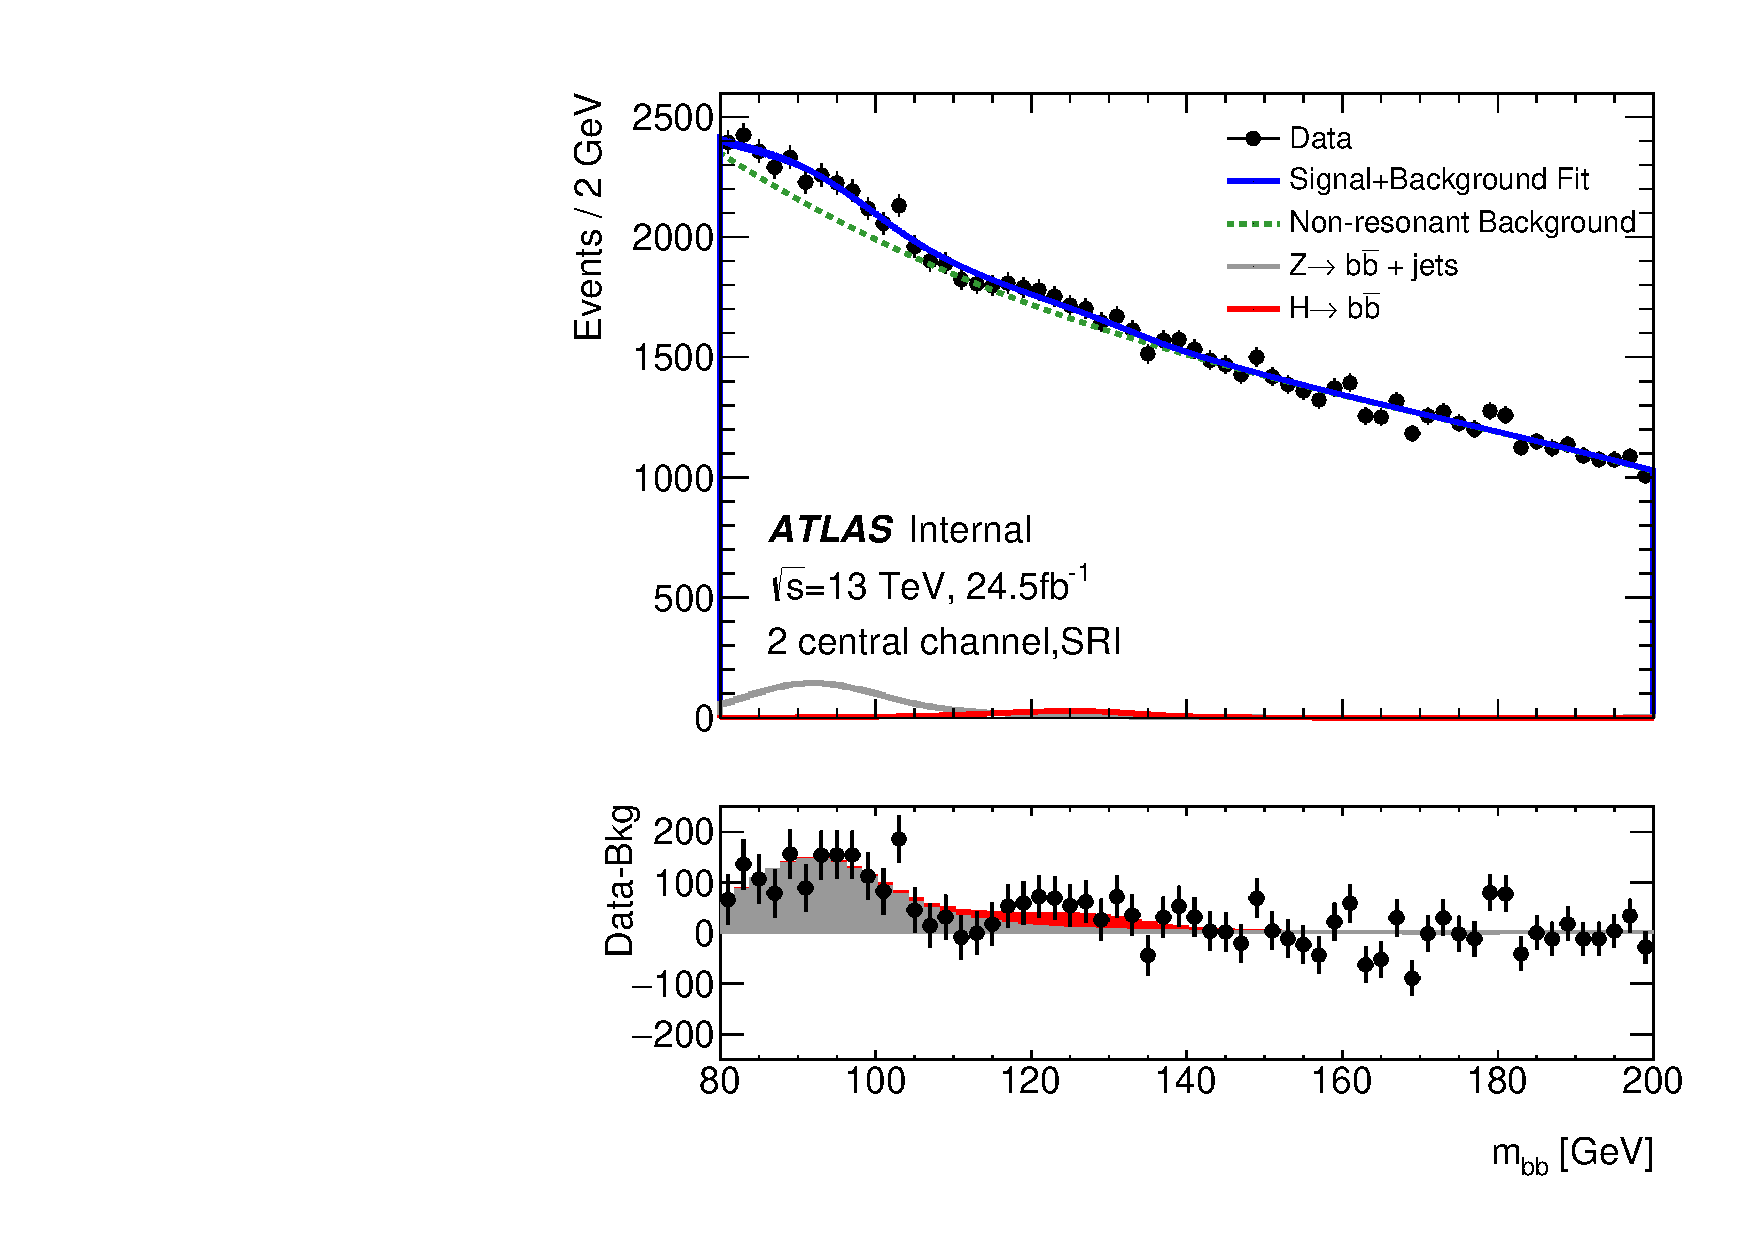
\includegraphics[width=0.48\textwidth]{figures/VBF/unblind_testVBF_ICHEP_2cen_SRI.pdf}
% 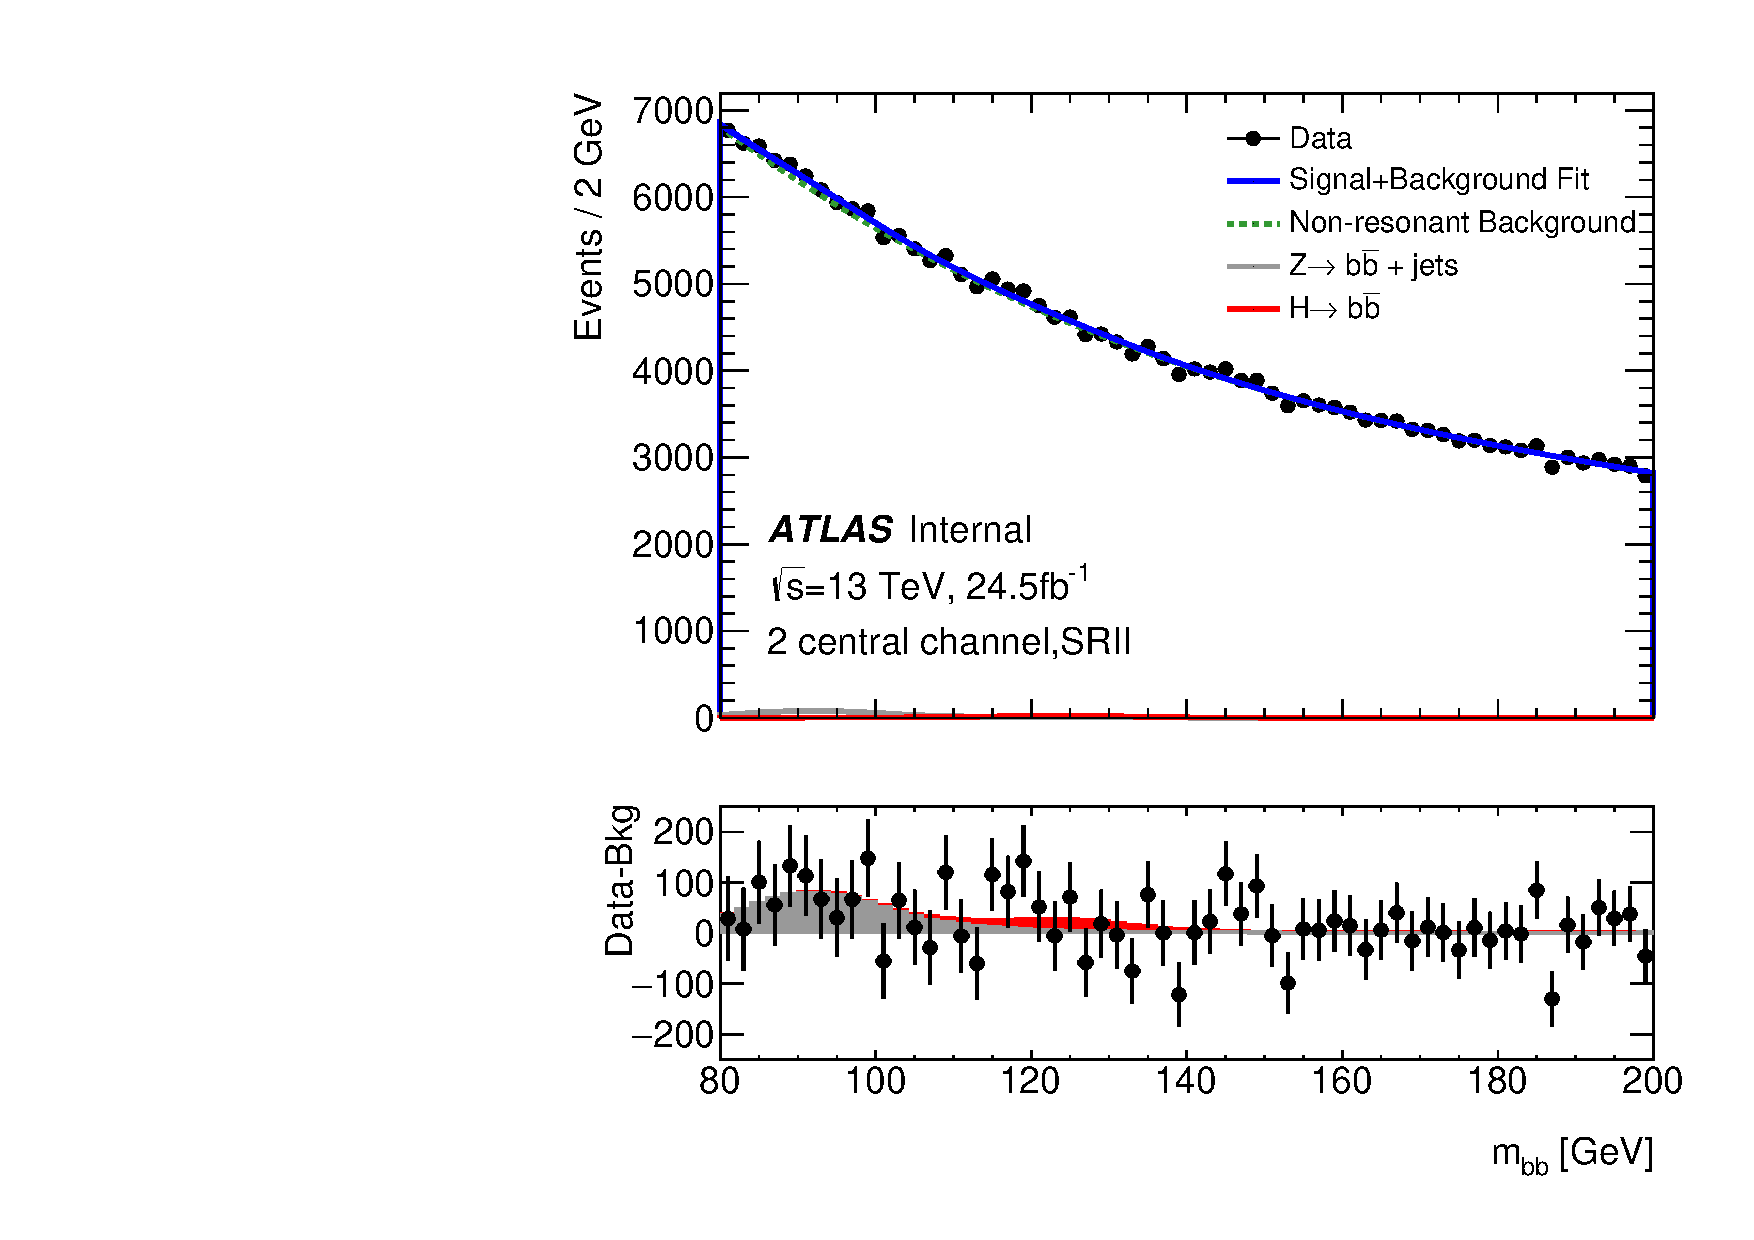
\includegraphics[width=0.48\textwidth]{figures/VBF/unblind_testVBF_ICHEP_2cen_SRII.pdf}\\
%\caption{Data and fit model comparison for profile likelihood fit in the \twocentral channel signal regions.  The fitted continuum background is shown with at  dashed green line, the fitted $Z$ signal in green, and the fitted Higgs signal in red.  The total fit is displayed as the blue line.  The bottom panels show the residual of the data with respect to the continuum background fit, and the fitted $Z$ signal (grey) and Higgs signal (red) are also displayed. }
%  \label{fig:vbf-higgsfit_2cen}
%\end{figure}
%
%\begin{figure}[htbp]
%  \centering
% 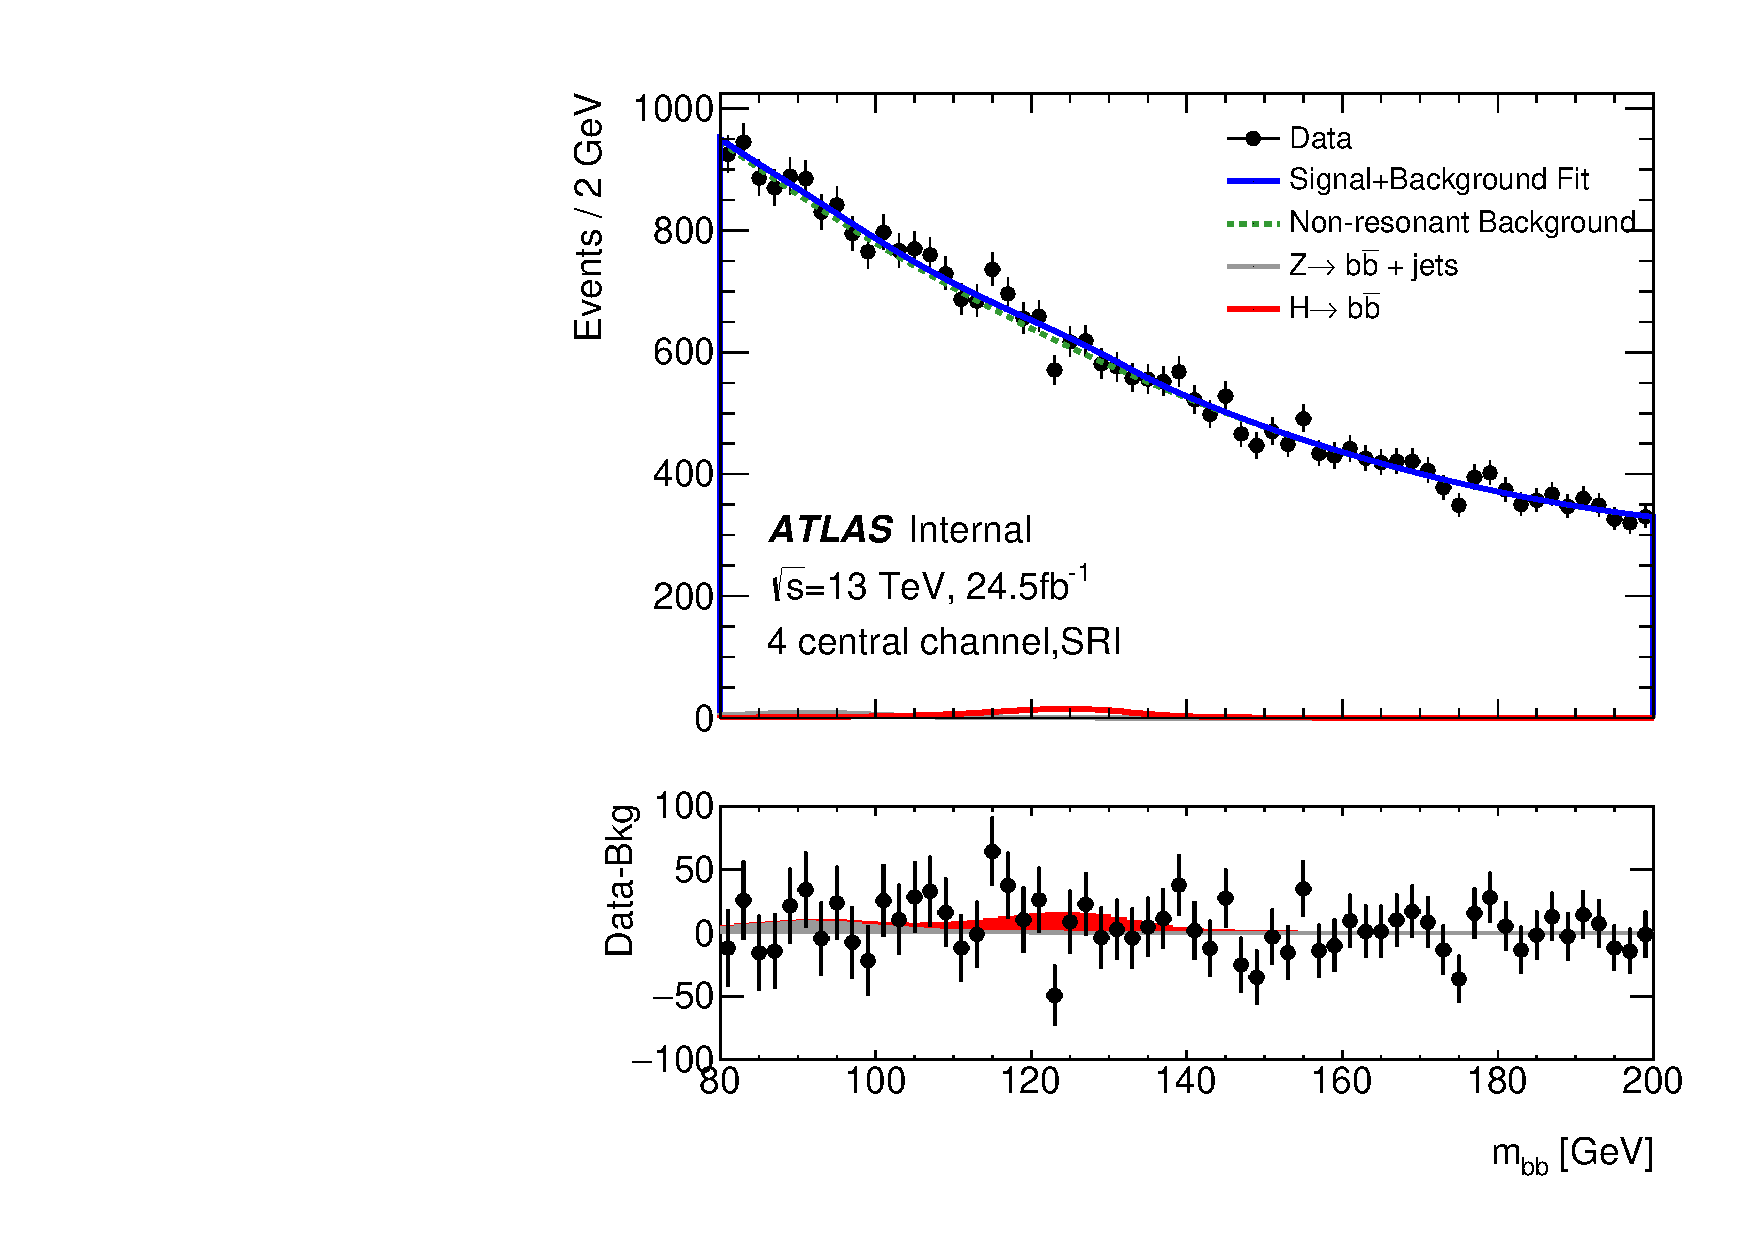
\includegraphics[width=0.48\textwidth]{figures/VBF/unblind_testVBF_ICHEP_4cen_SRI.pdf}
% 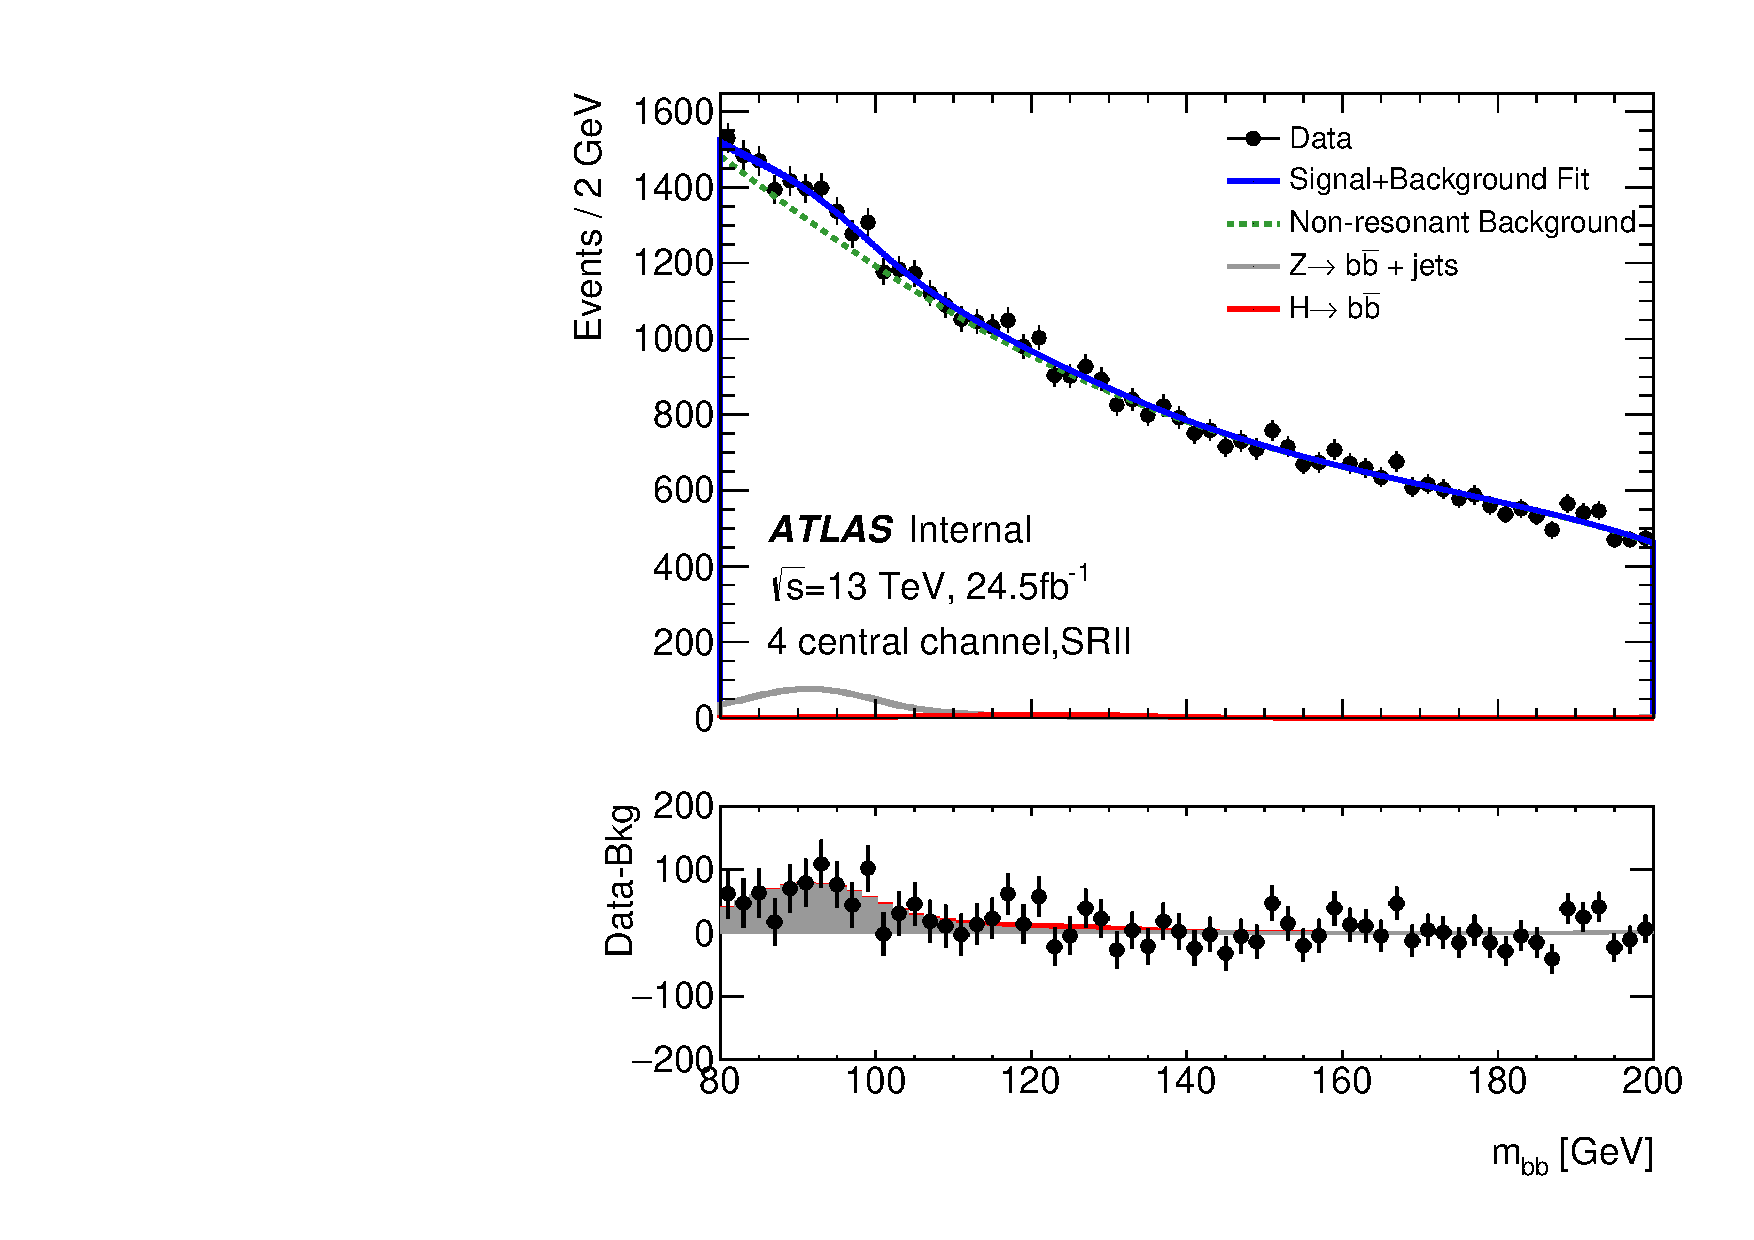
\includegraphics[width=0.48\textwidth]{figures/VBF/unblind_testVBF_ICHEP_4cen_SRII.pdf}\\
% 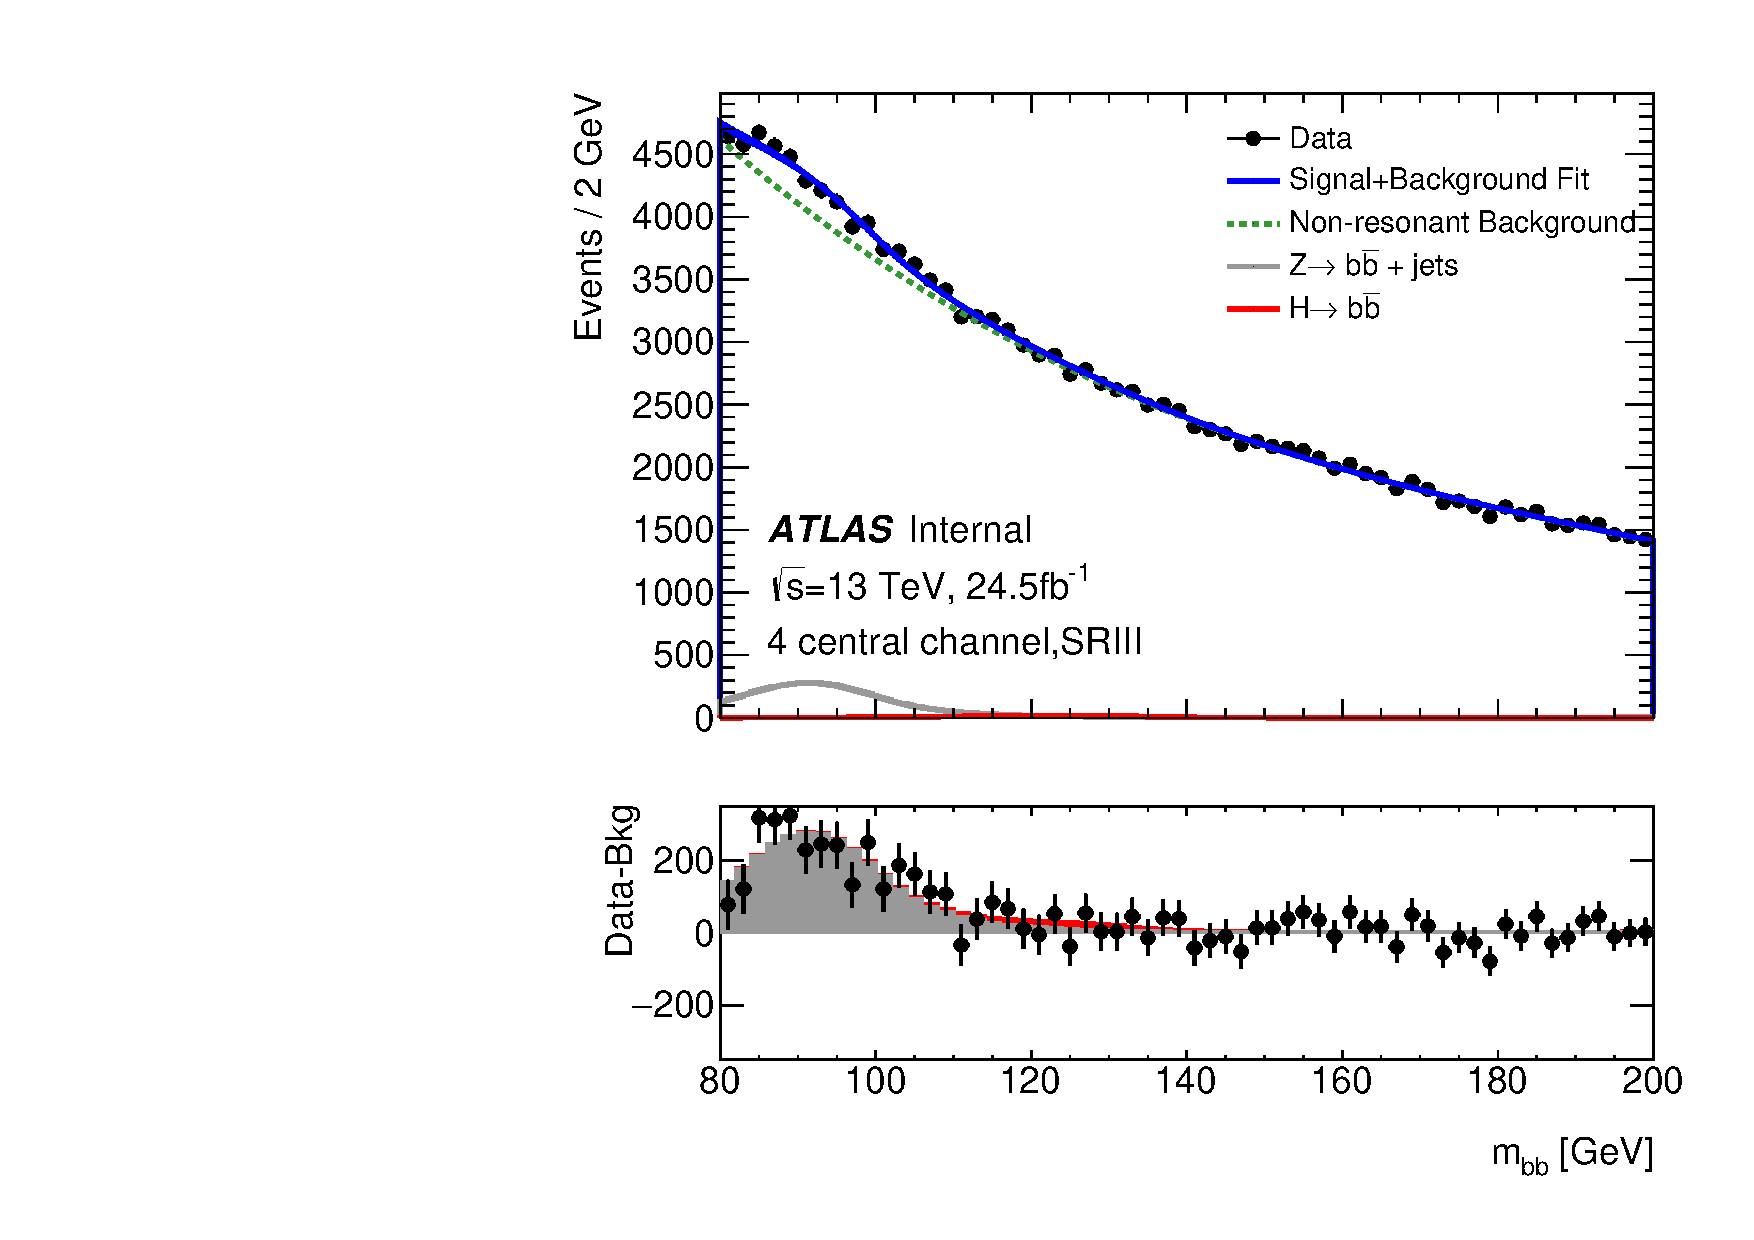
\includegraphics[width=0.48\textwidth]{figures/VBF/unblind_testVBF_ICHEP_4cen_SRIII.pdf}
% 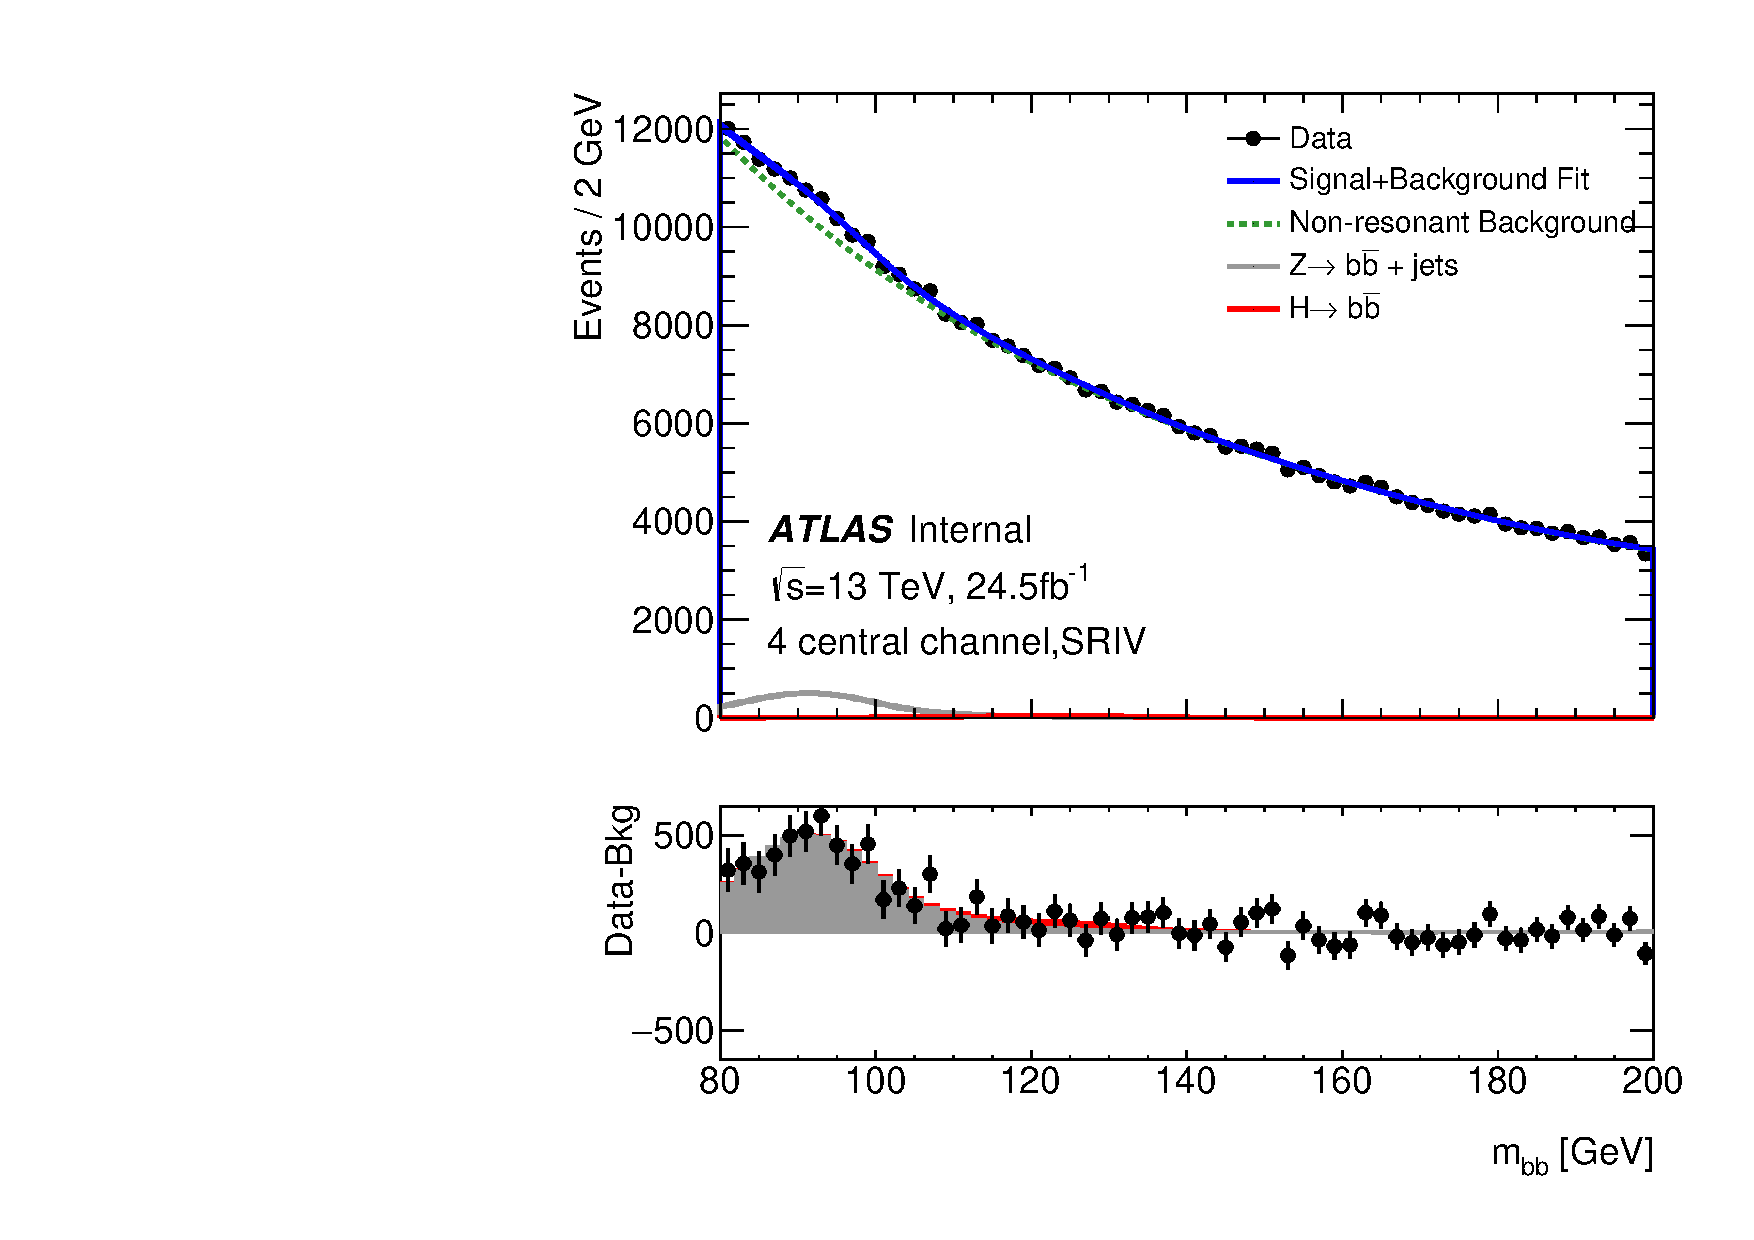
\includegraphics[width=0.48\textwidth]{figures/VBF/unblind_testVBF_ICHEP_4cen_SRIV.pdf}\\
%\caption{Data and fit model comparison for profile likelihood fit in the \fourcentral channel signal regions. The fitted continuum background is shown with at  dashed green line, the fitted $Z$ signal in green, and the fitted Higgs signal in red.  The total fit is displayed as the blue line.  The bottom panels show the residual of the data with respect to the continuum background fit, and the fitted $Z$ signal (grey) and Higgs signal (red) are also displayed.}
%  \label{fig:vbf-higgsfit_4cen}
%\end{figure}


\subsection{Extraction of $\mu_{VBF}$}
\label{sec:vbf-higgsunblindvbf}
A different interpretation of the analysis is the extraction of $\mu_{VBF}$ signal strength.
The fit procedure follows the same way as the extraction of $\mu_{H}$, except we only float
the $VBF$ signal in the fit while fixing the yield of all other Higgs modes, i.e. ggF,
ttH and VH to their Standard Model predictions (with uncertainties applied).
The Asimov fit yields $\mu_{VBF}=1\pm 2.8$. The unblinded value of the VBF Higgs signal
strength is $4.1^{+3.2}_{-2.9}$. The breakdown of the uncertainty
is $\mu_{VBF}=4.1^{+2.8}_{-2.8}\textnormal{(stat)}^{+1.5}_{-0.8}\textnormal{(syst)}$ treating
the NPs for the analytical background parameterization and normalization as well as
the normalization of $Z$ contribution as statistical uncertainty.


\subsubsection{Combination with VBF$+\gamma$ Analysis}
\label{sec:vbf-higgscomb}

The combination of the all-hadronic VBF analysis and the
VBF$+\gamma$ analysis~\cite{vbfplusgammaint} is performed
by a simultaneous likelihood fit to both datasets. The Higgs signal strength is
treated as correlated across all analysis regions,
the $Z$ contributions are extracted as described in the respective analyses.
As described in Section~\ref{sec:vbf-presel}, overlap between the two samples is removed.

The combined fit yields $\mu_H = 2.5^{+1.4}_{-1.3}$ corresponding to an observed significance
of $1.9\sigma$ ($0.8\sigma$ expected). The $VBF$ signal only extraction is also performed combining two analyses similar to \ref{sec:vbf-higgsunblindvbf}. The combined fit yields $\mu_{VBF} =3.0^{+1.7}_{-1.6}$ corresponding to an observed significance of $1.9\sigma$ ($0.7\sigma$ expected). The data and fit model comparisons for $\mu_{VBF}$ extraction are shown in Fig.\ref{fig:higgsfit_2cen},\ref{fig:higgsfit_4cen},\ref{fig:mbb_postfit_photon}.

The extractions of $\mu_{H}$ and $\mu_{VBF}$ for separate fits of both all-hadronic and photon analysis and the combination fit are summarized in Fig.\ref{fig:vbf-summary}.


\begin{figure}[htbp]
  \centering
 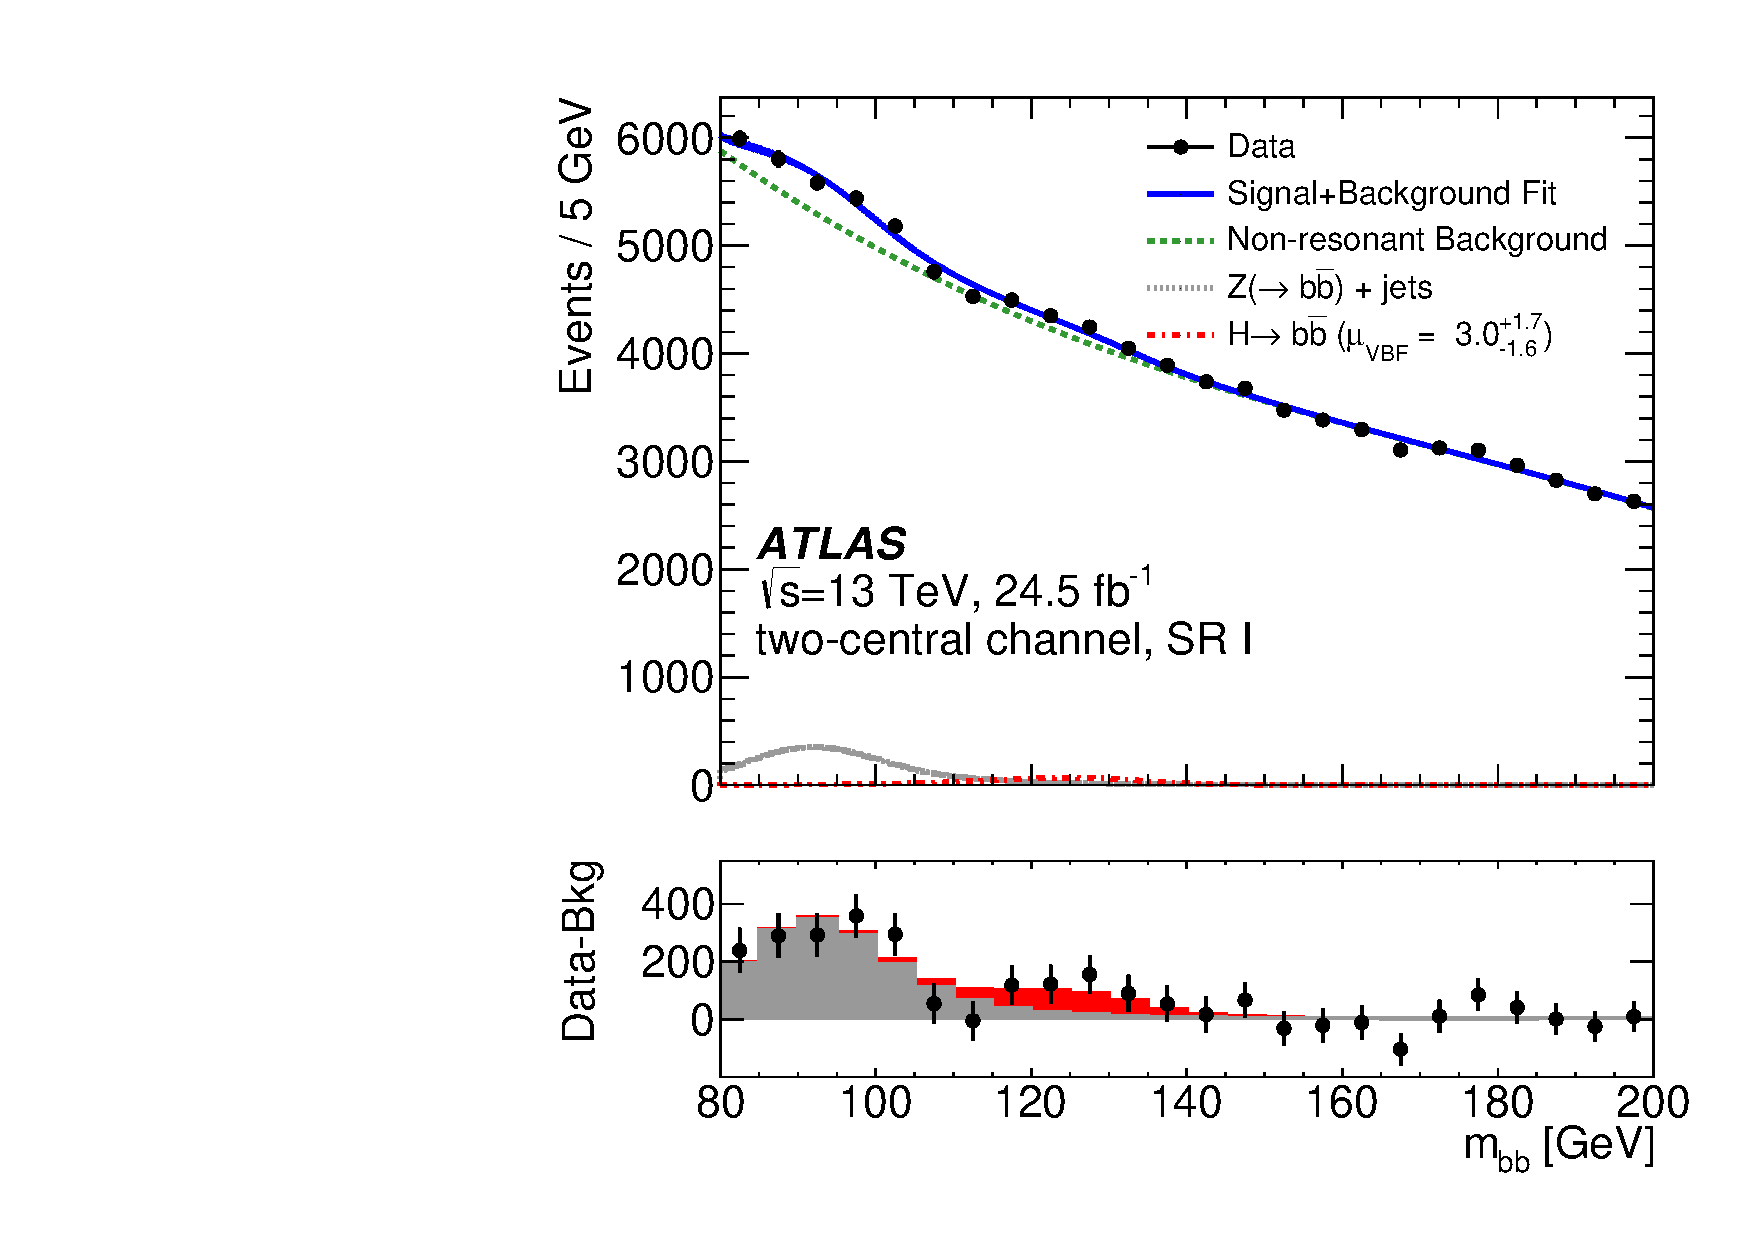
\includegraphics[width=0.48\textwidth]{figures/VBF/comb_vbfonly_testVBF_ICHEP_2cen_SRI_vbfincl.pdf}
 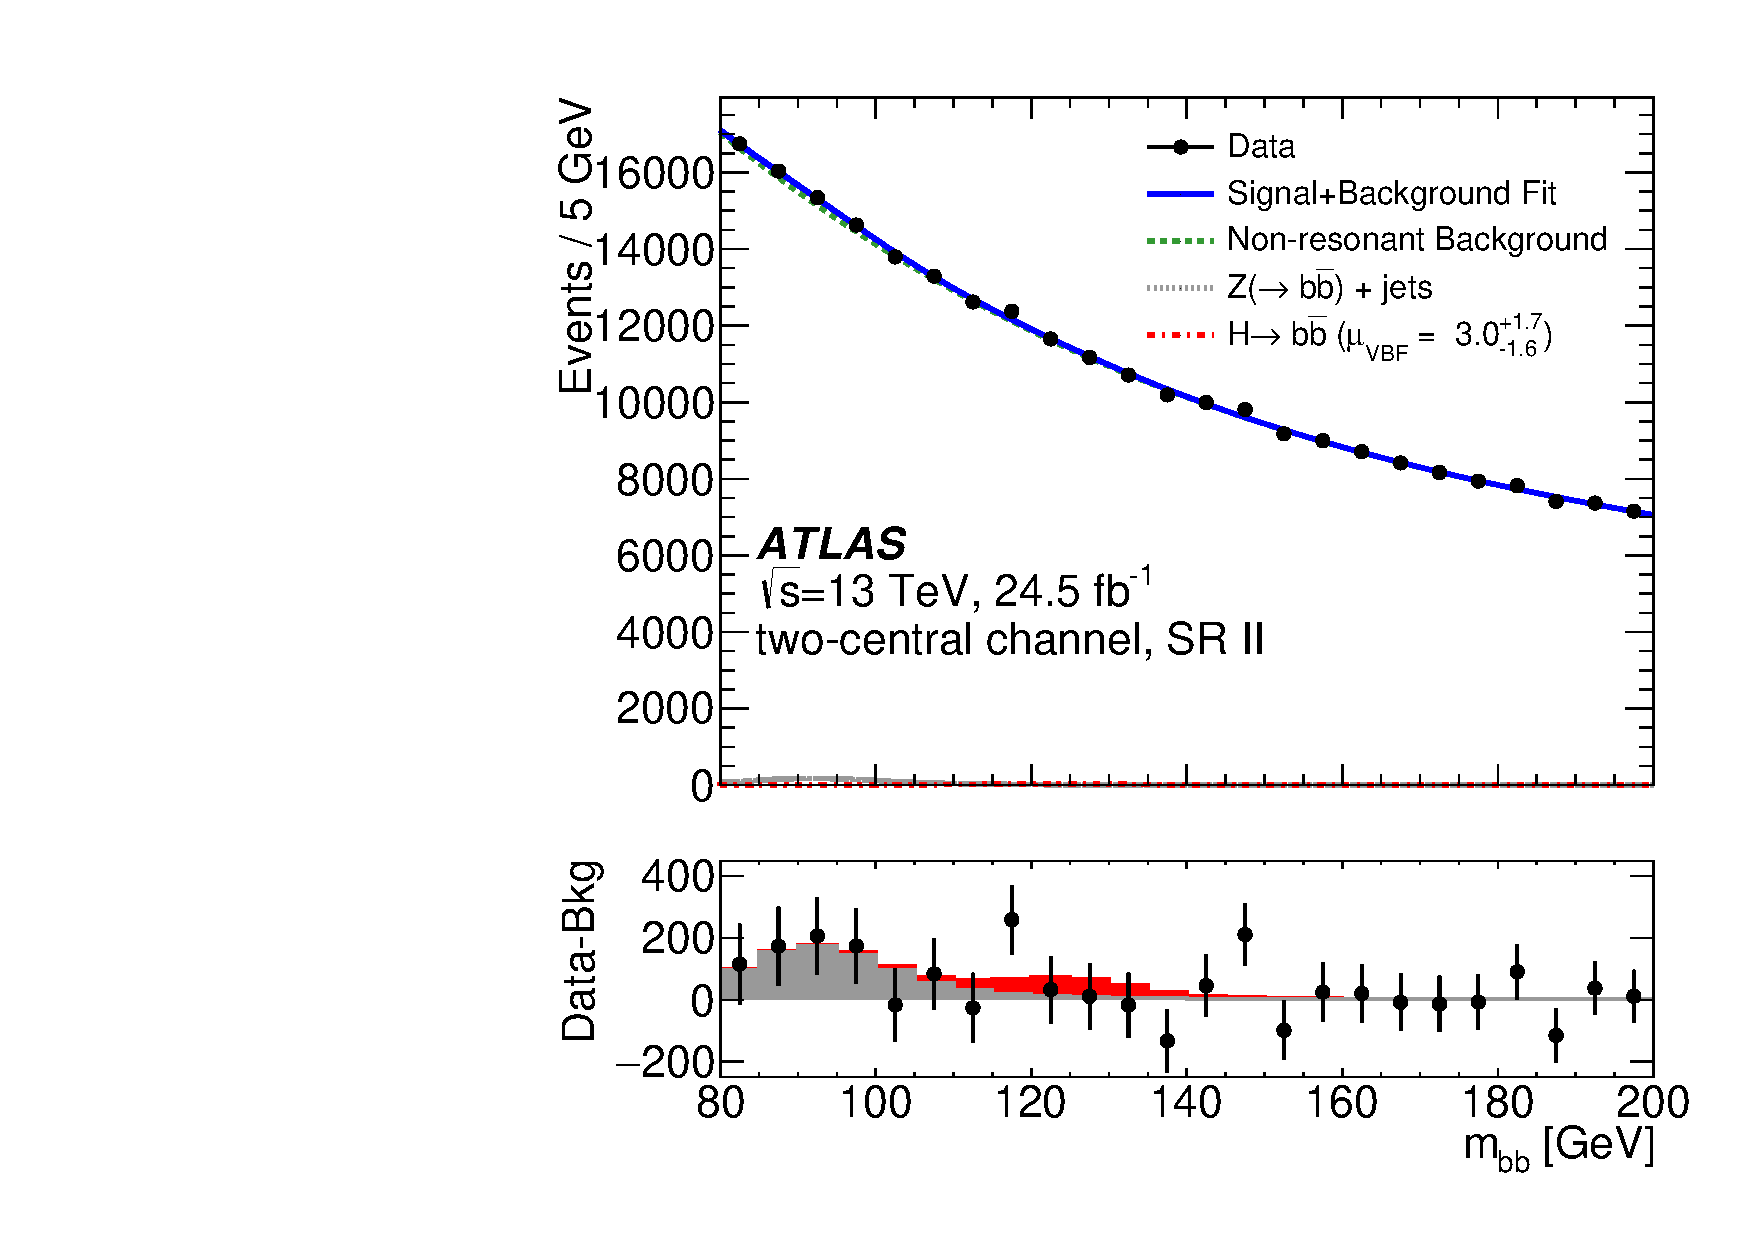
\includegraphics[width=0.48\textwidth]{figures/VBF/comb_vbfonly_testVBF_ICHEP_2cen_SRII_vbfincl.pdf}\\

\caption{Data and fit model comparison for the combined fit of $\mu_{VBF}$ extraction in the \twocentral channel}
  \label{fig:higgsfit_2cen}
\end{figure}

\begin{figure}[htbp]
  \centering
  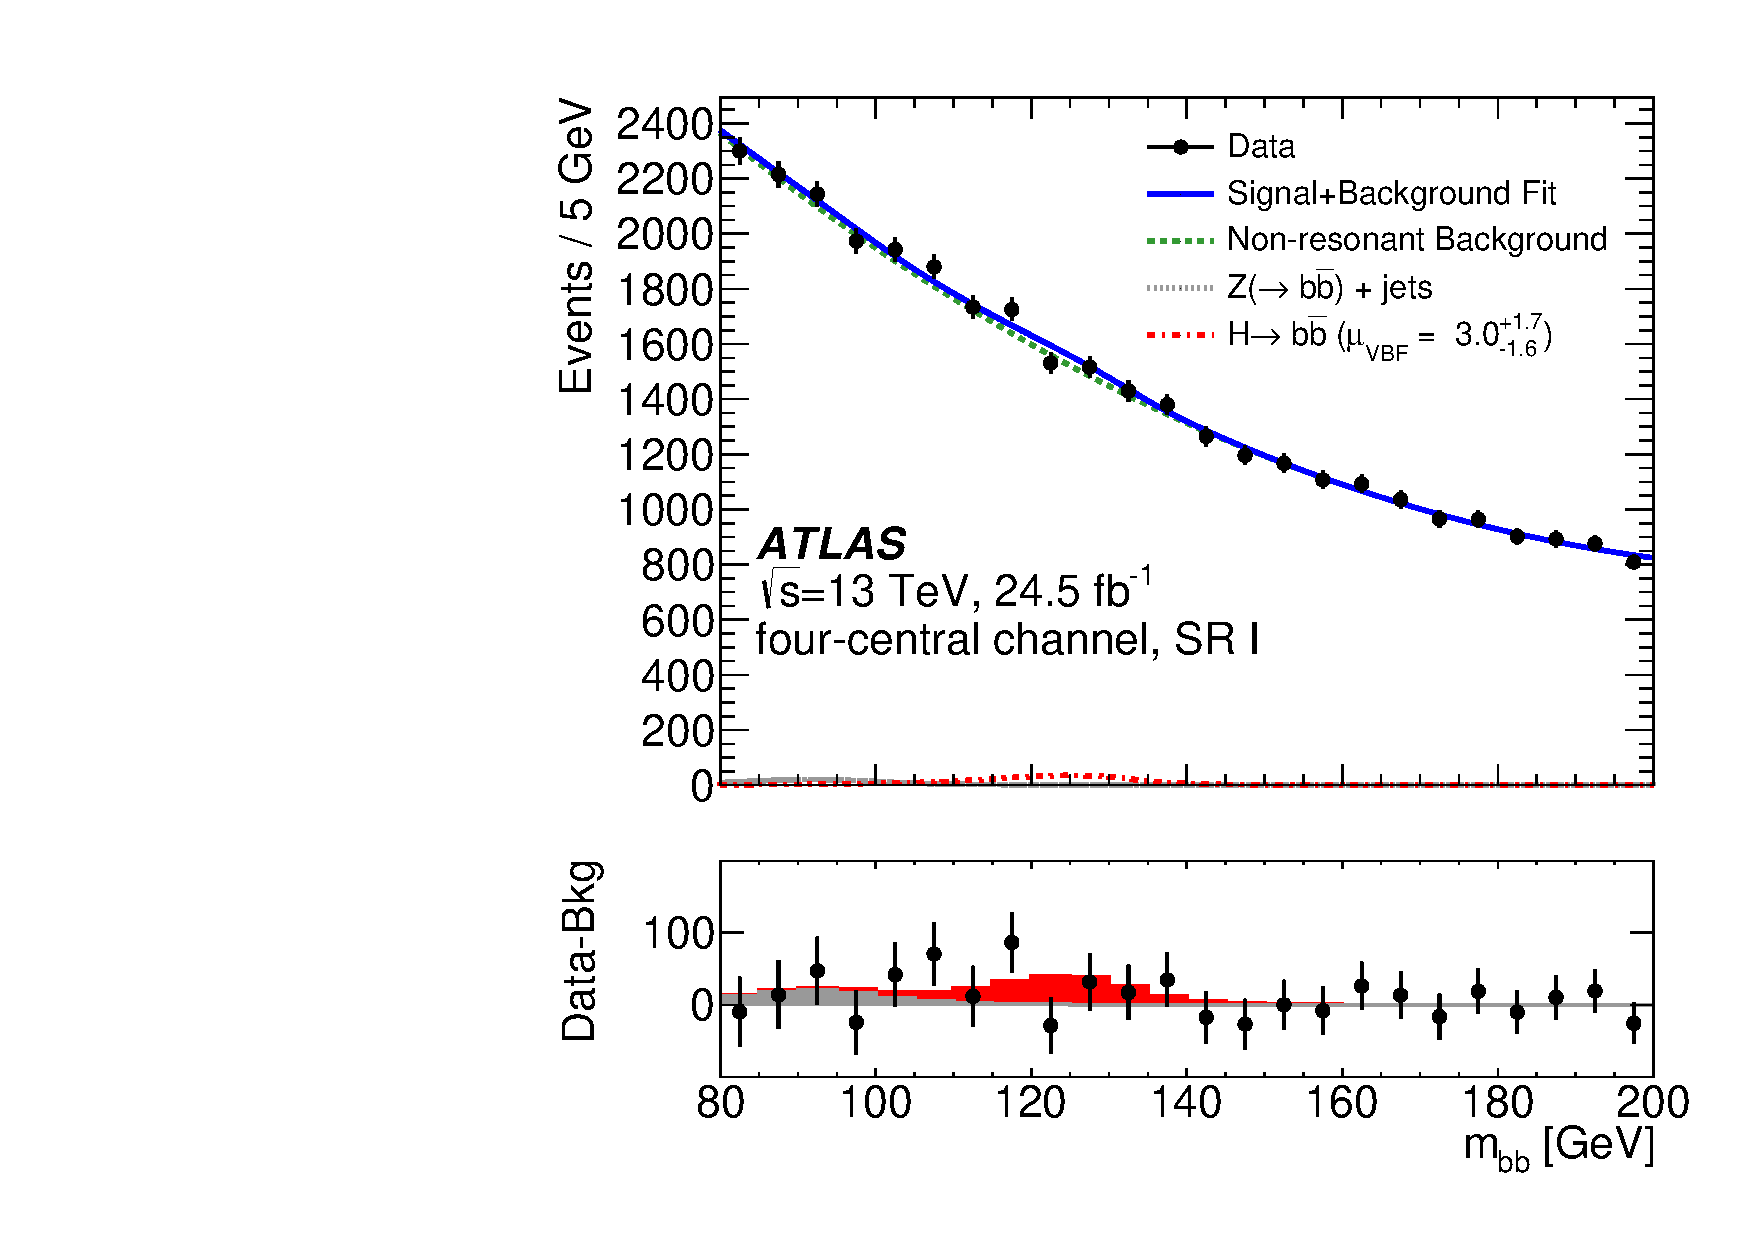
\includegraphics[width=0.48\textwidth]{figures/VBF/comb_vbfonly_testVBF_ICHEP_4cen_SRI_vbfincl.pdf}
 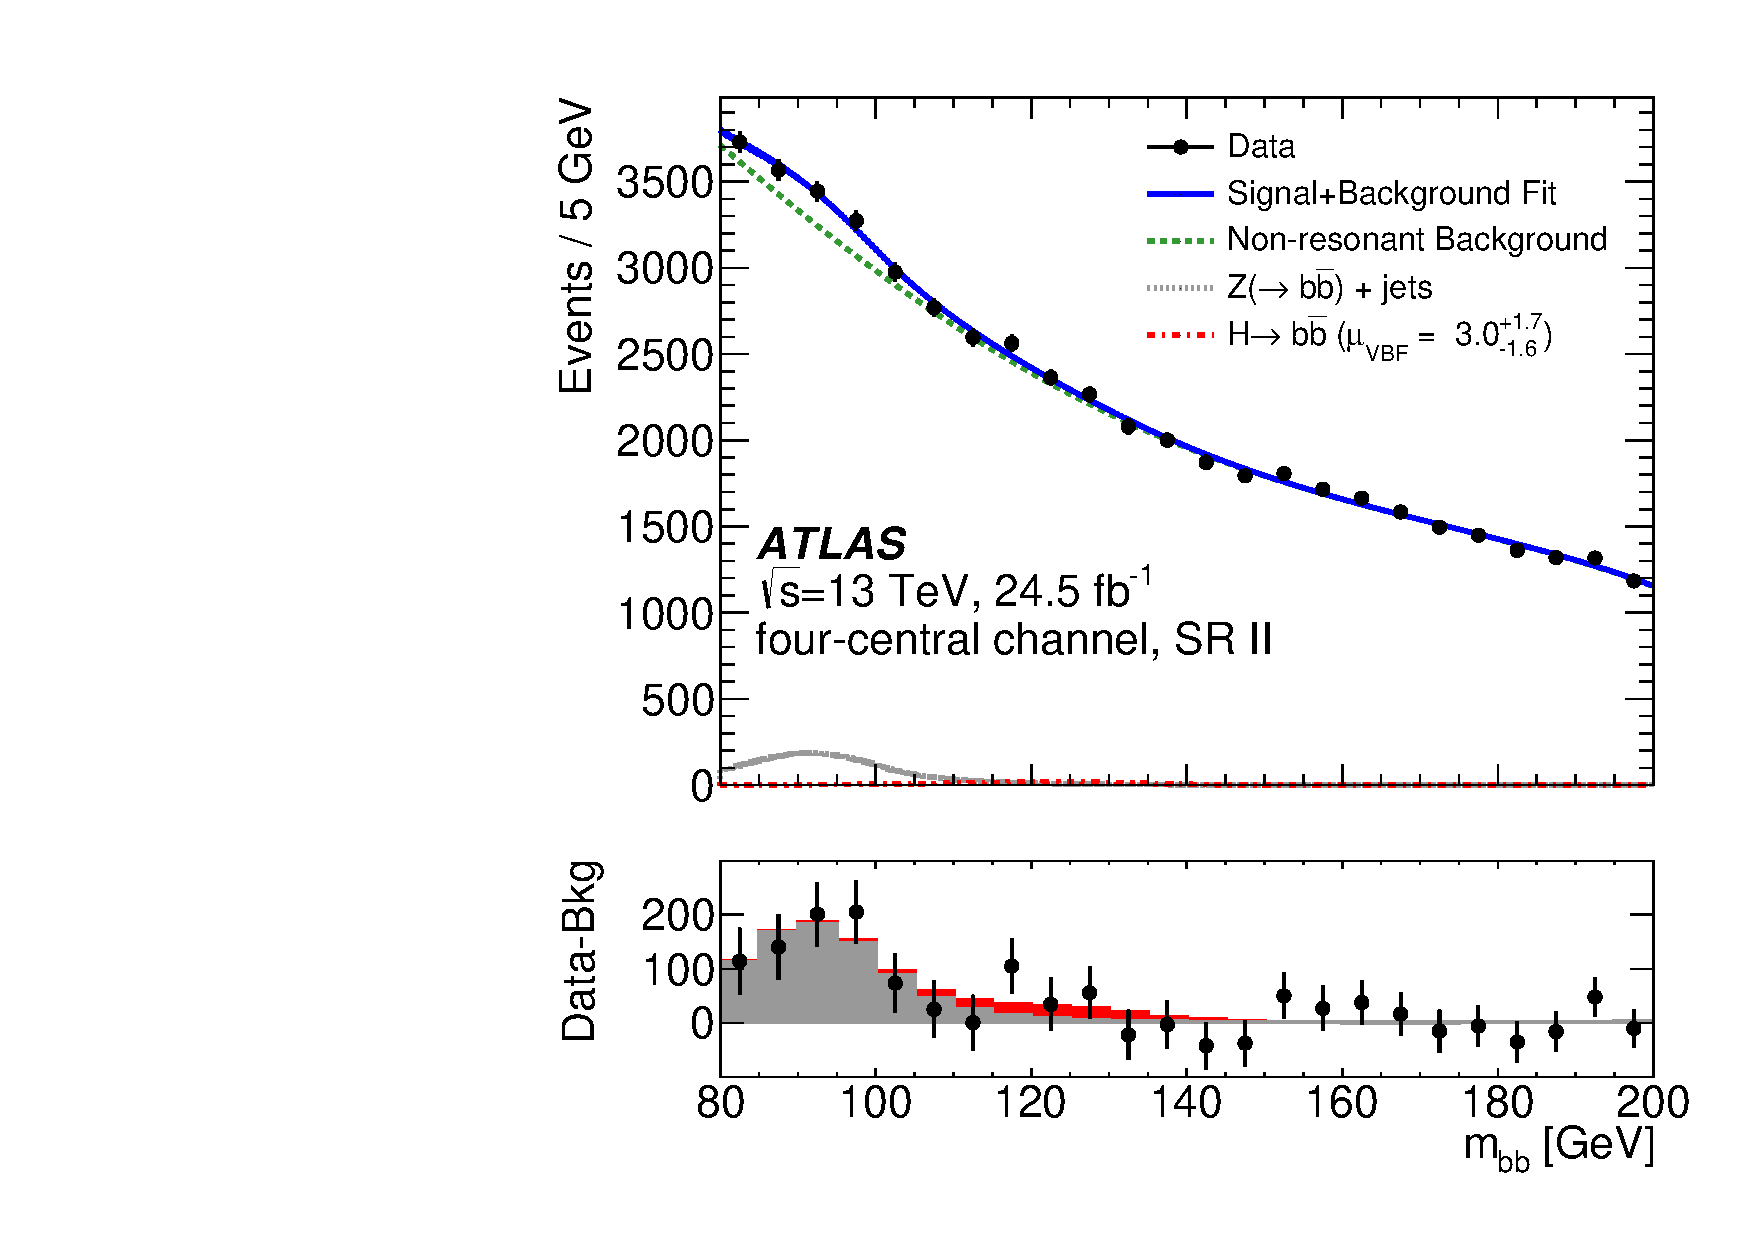
\includegraphics[width=0.48\textwidth]{figures/VBF/comb_vbfonly_testVBF_ICHEP_4cen_SRII_vbfincl.pdf}\\
 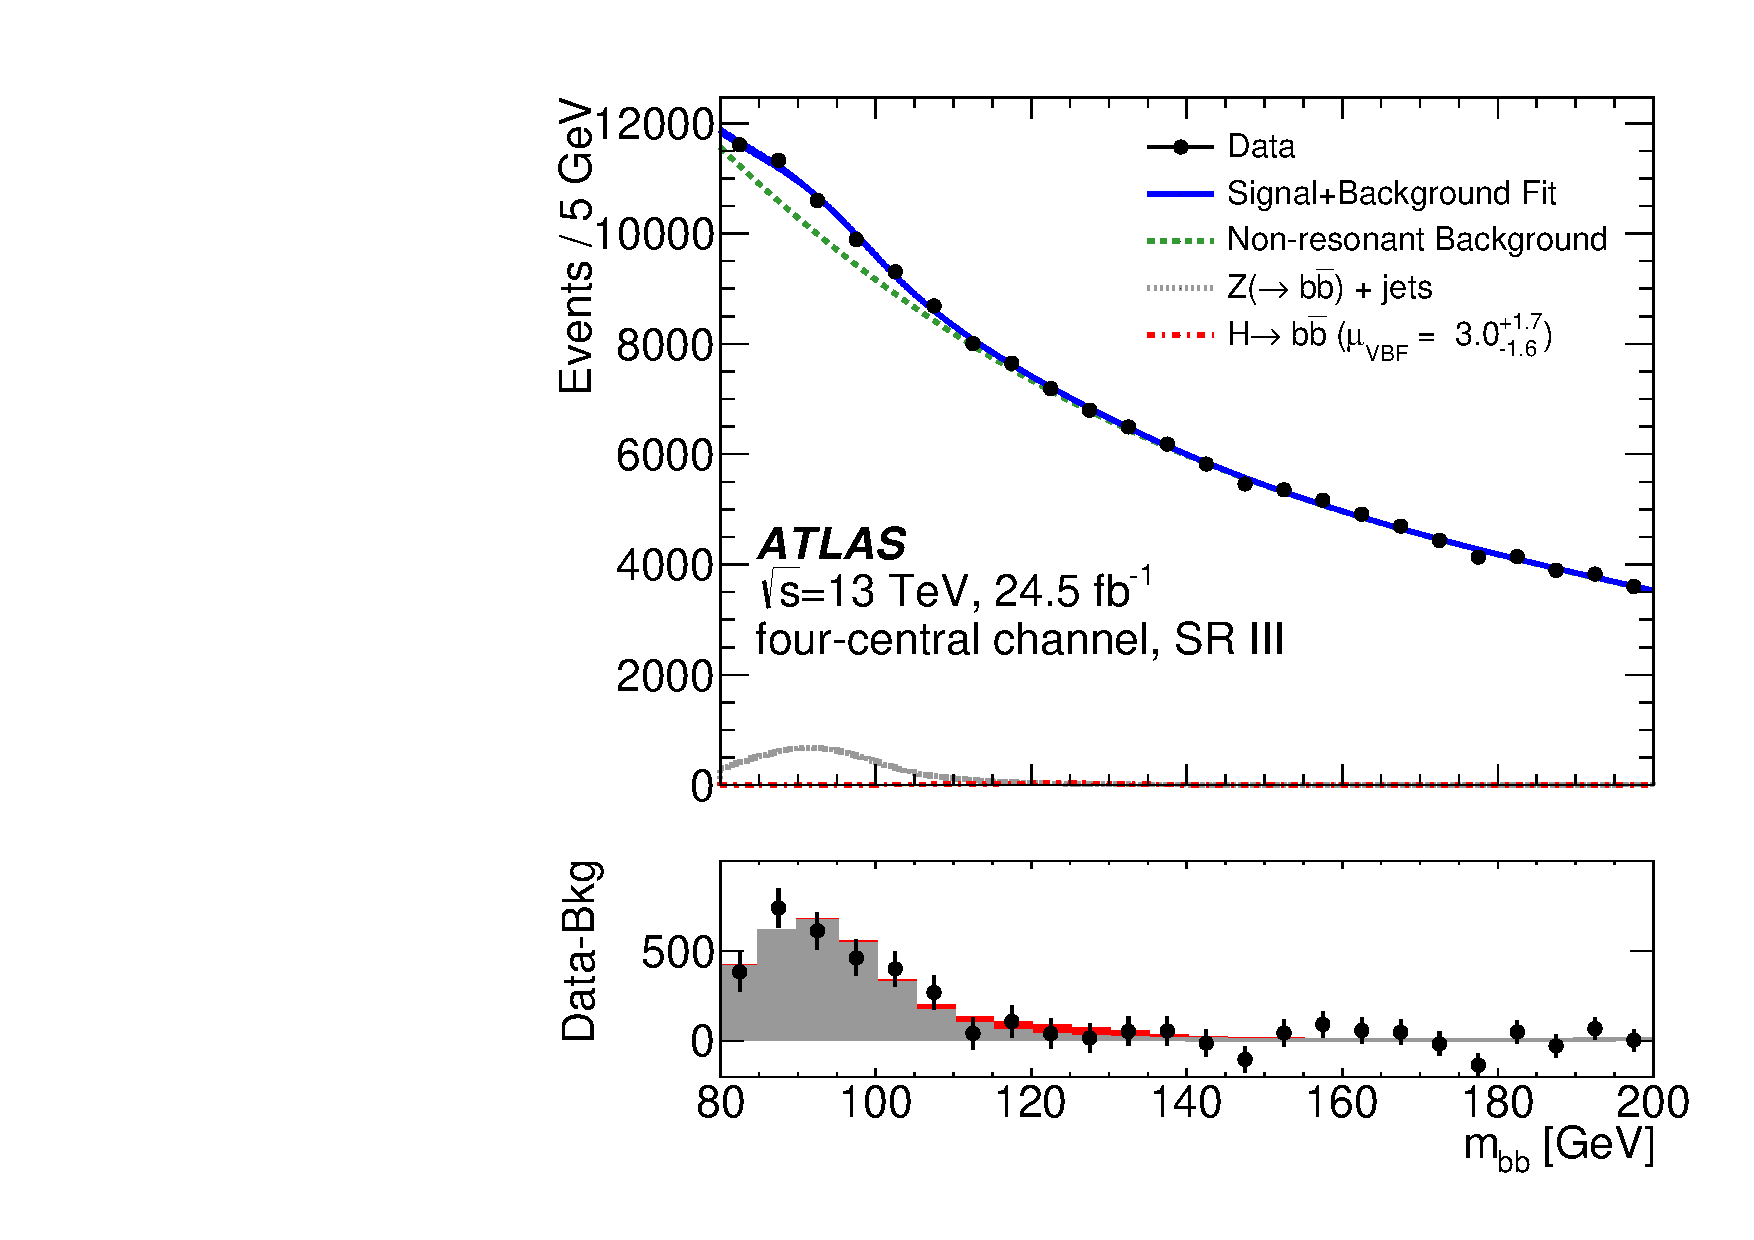
\includegraphics[width=0.48\textwidth]{figures/VBF/comb_vbfonly_testVBF_ICHEP_4cen_SRIII_vbfincl.pdf}
 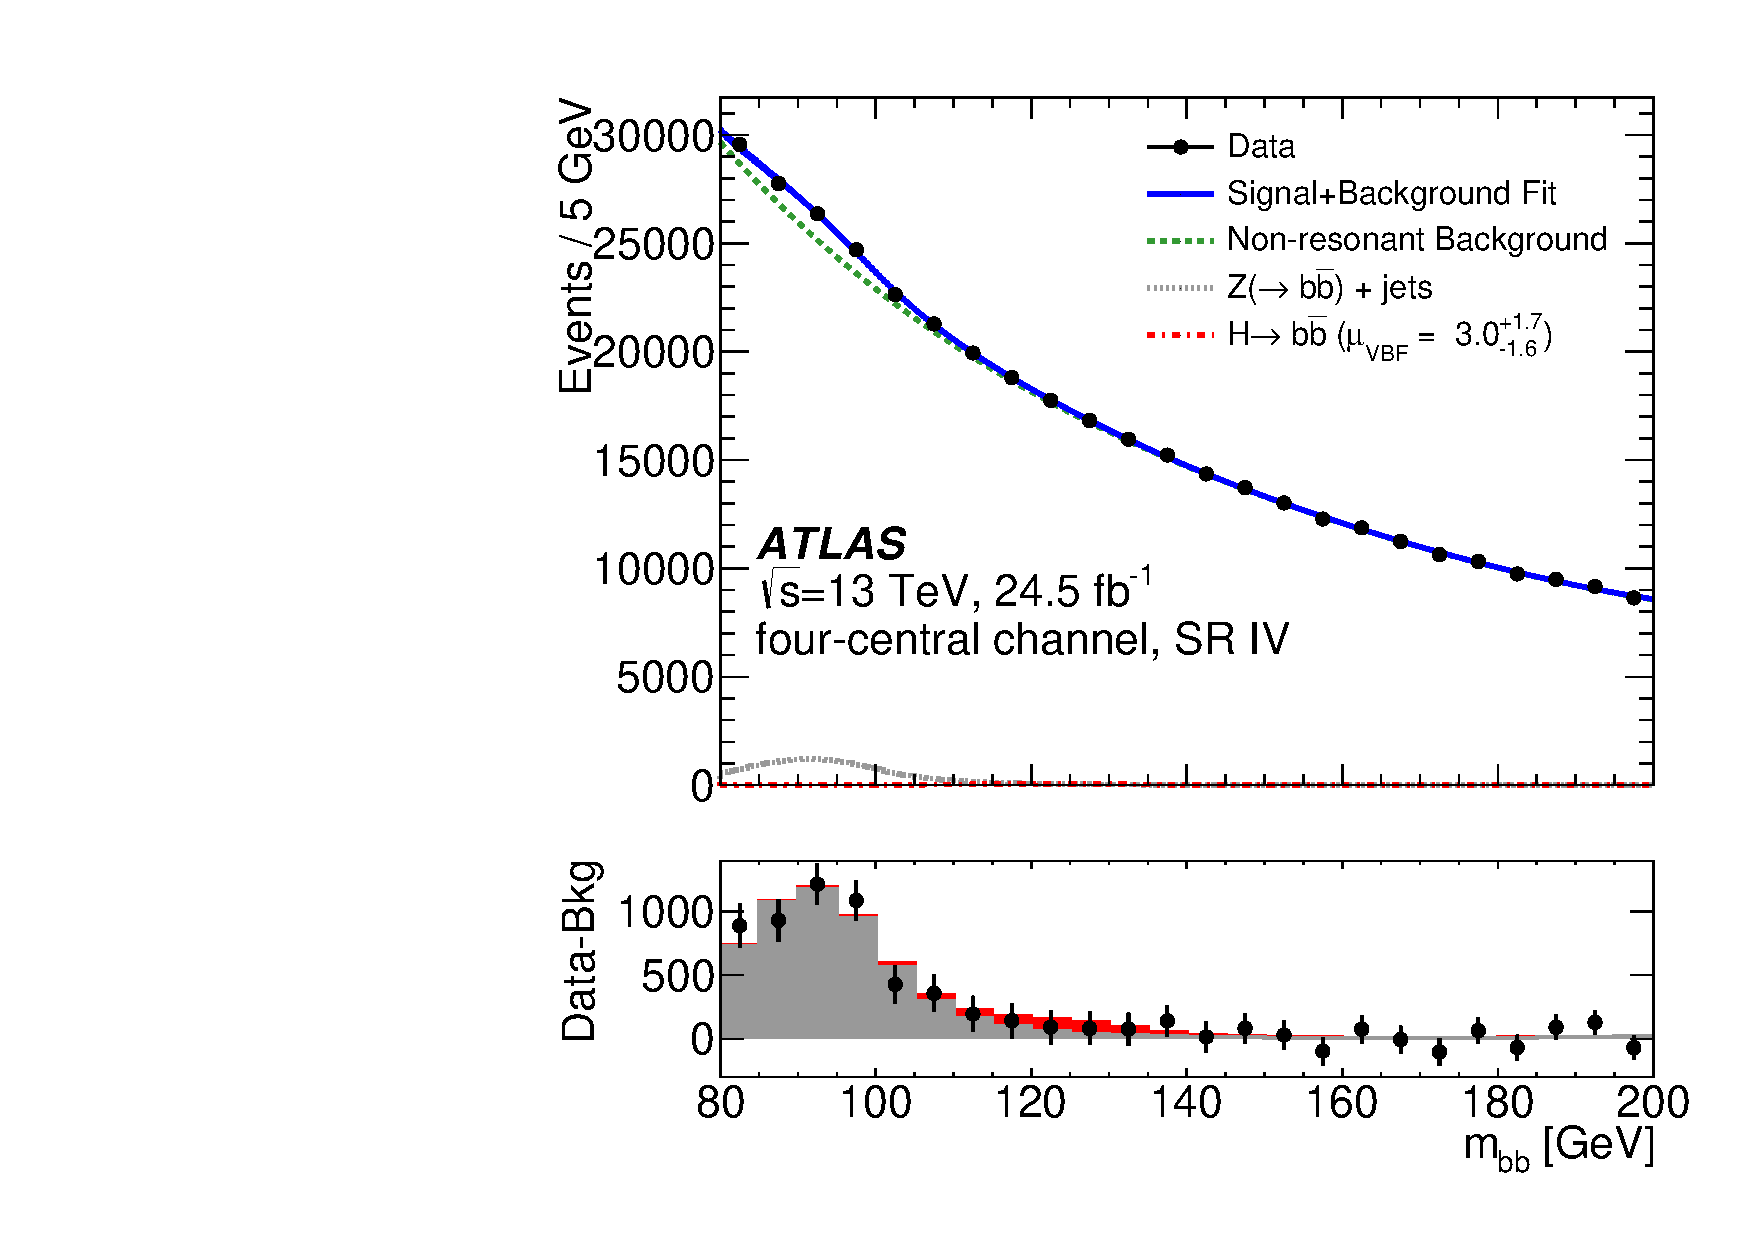
\includegraphics[width=0.48\textwidth]{figures/VBF/comb_vbfonly_testVBF_ICHEP_4cen_SRIV_vbfincl.pdf}\\

\caption{Data and fit model comparison for the combined fit of $\mu_{VBF}$ extraction in the \fourcentral channel}
  \label{fig:higgsfit_4cen}
\end{figure}



\begin{figure}[htbp]
\centering

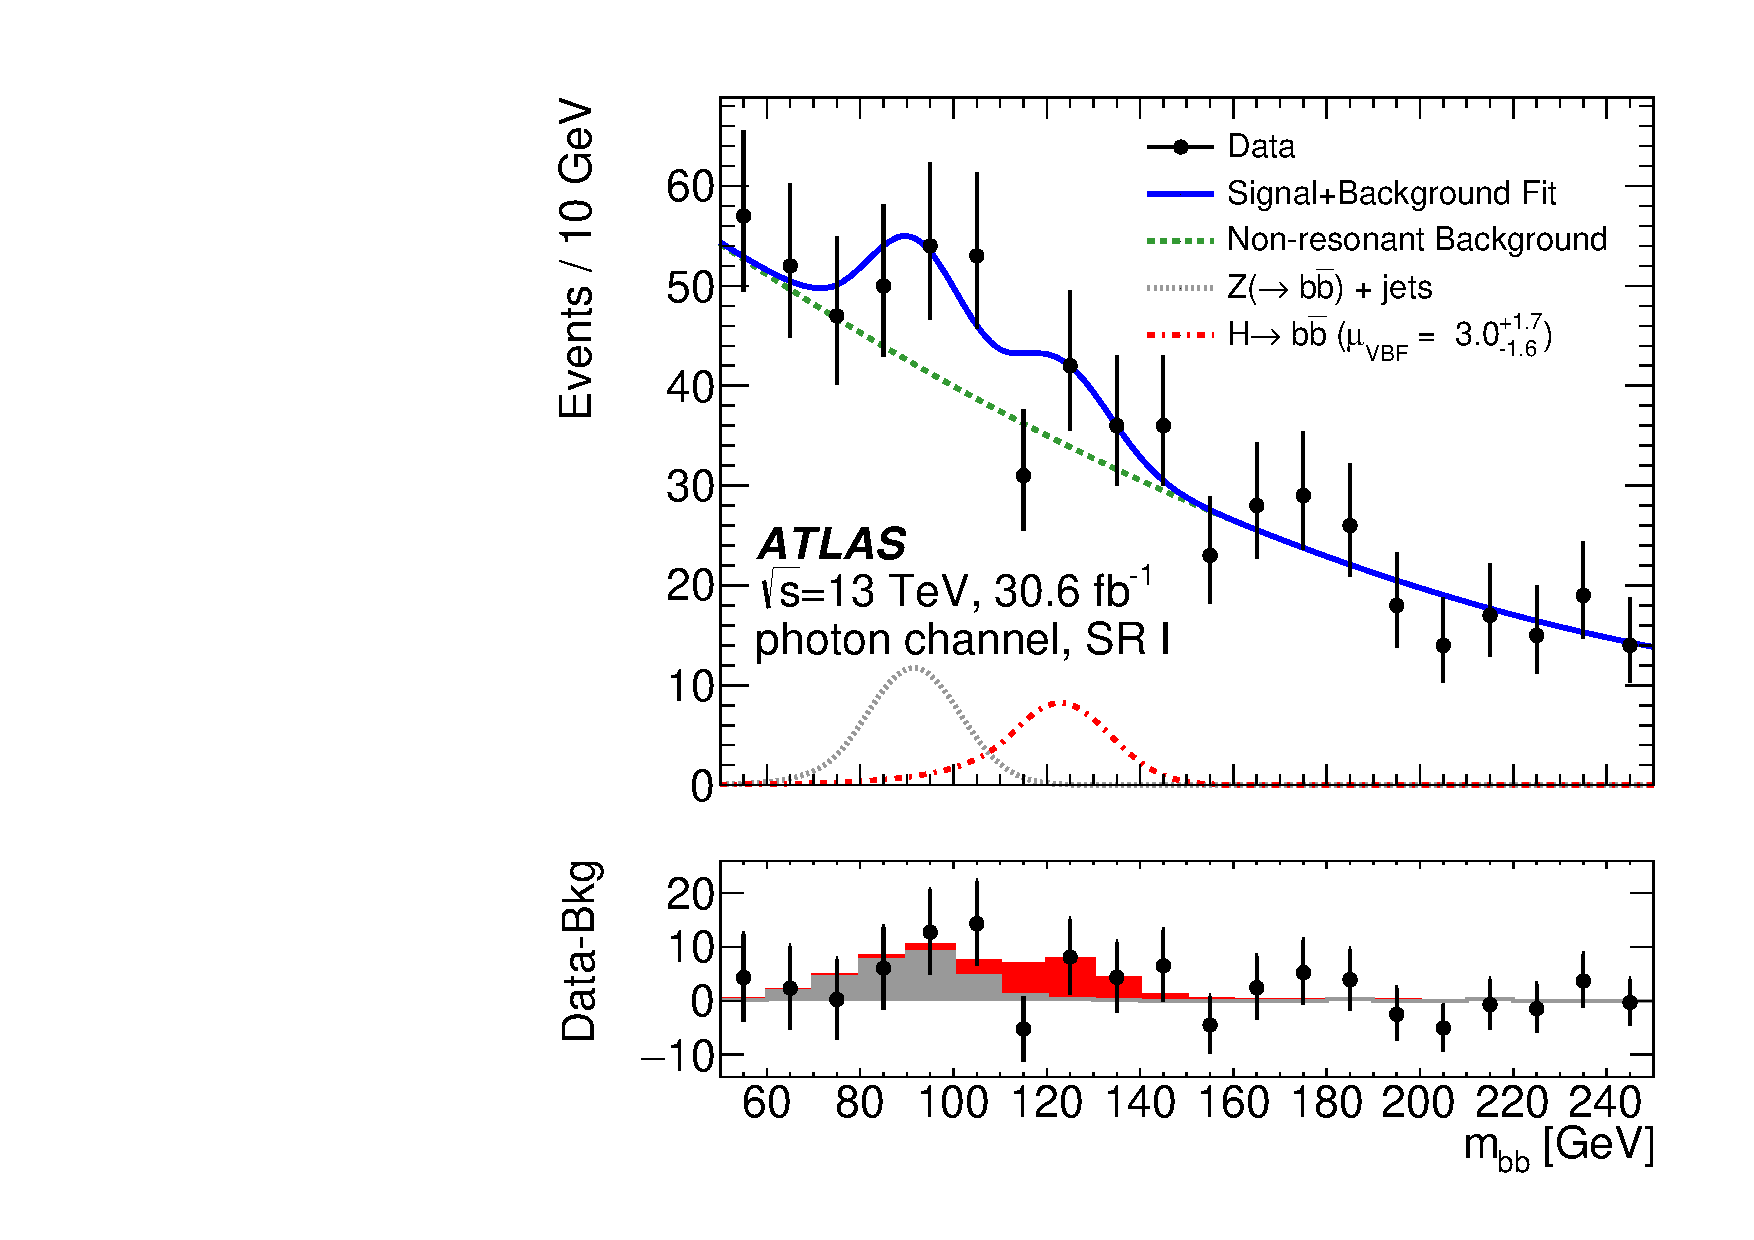
\includegraphics[width=0.48\textwidth]{figures/VBF/comb_vbfonly_testchannel1_vbfg.pdf}
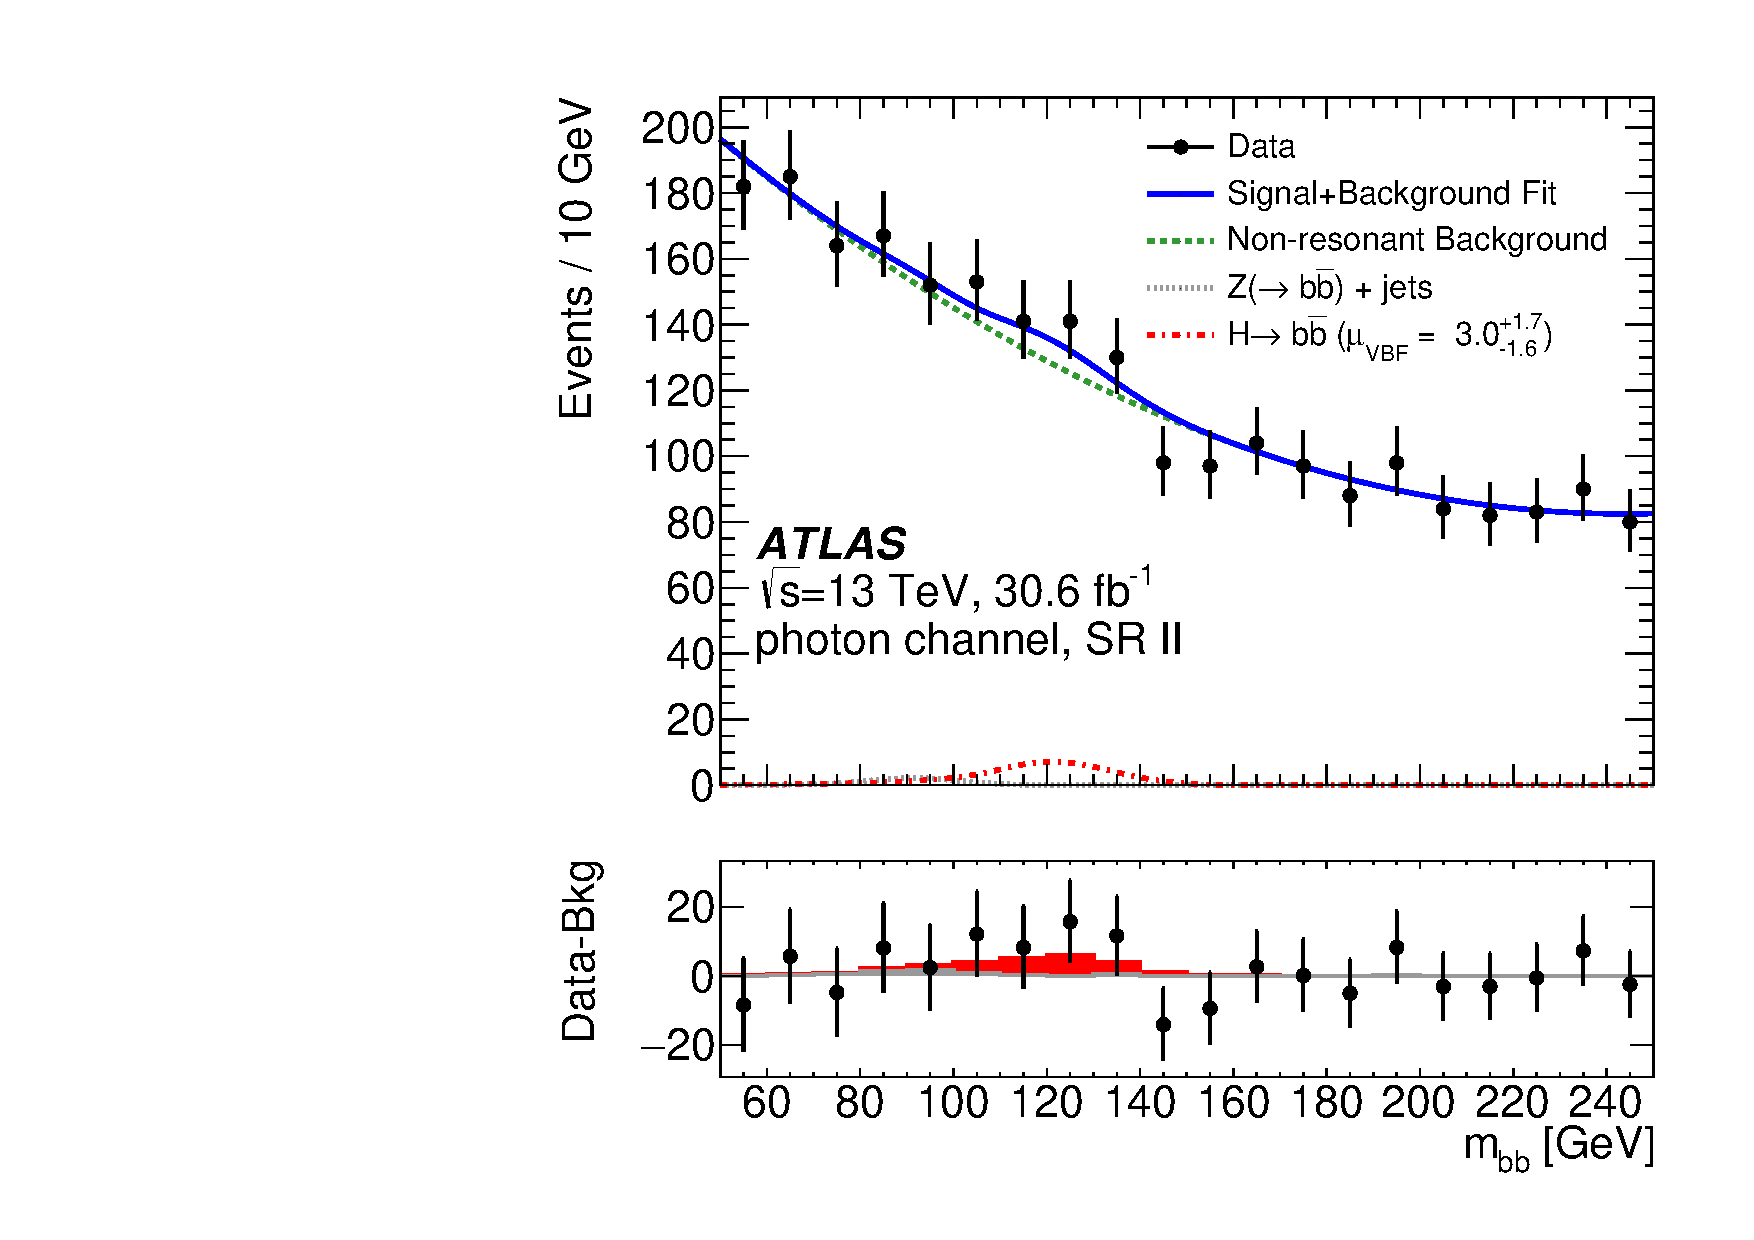
\includegraphics[width=0.48\textwidth]{figures/VBF/comb_vbfonly_testchannel2_vbfg.pdf}
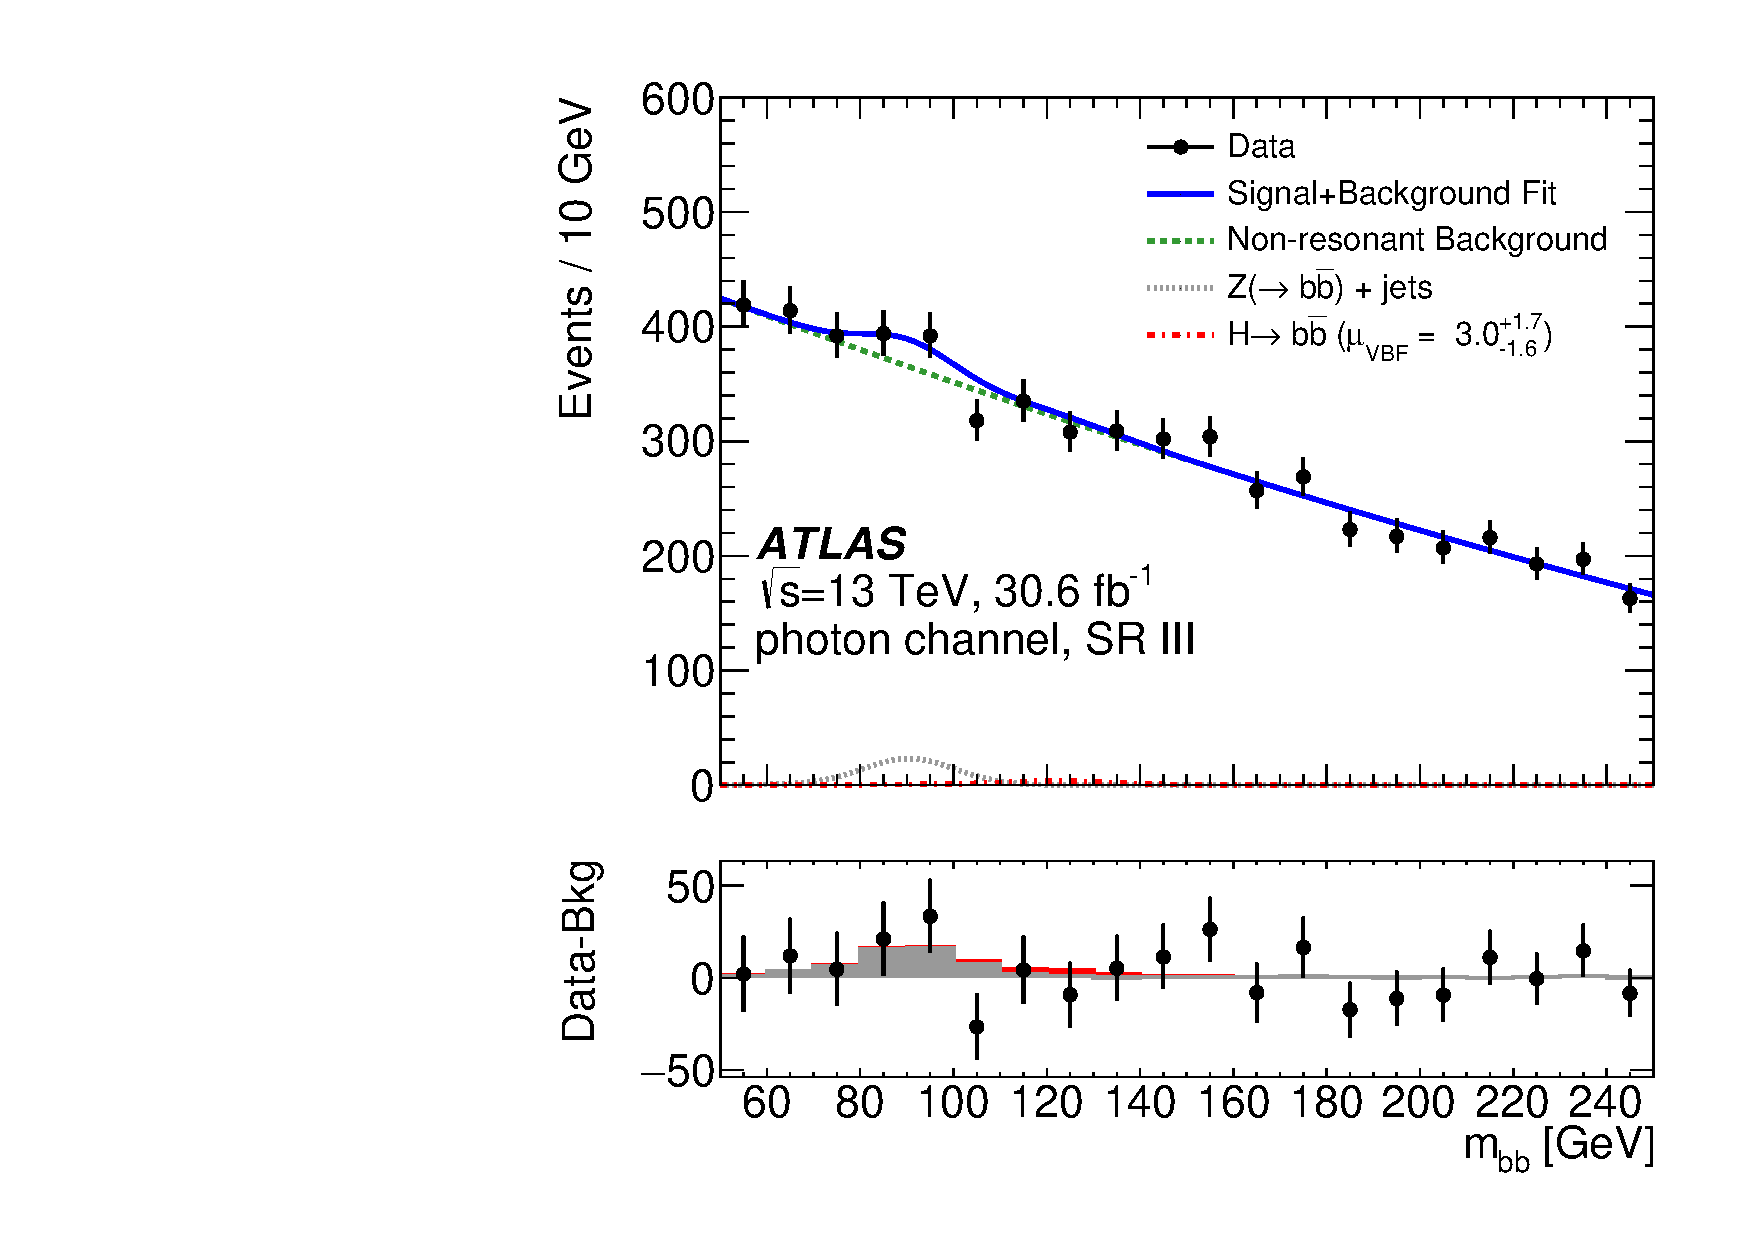
\includegraphics[width=0.48\textwidth]{figures/VBF/comb_vbfonly_testchannel3_vbfg.pdf}
\caption{Data and fit model comparison for the combined fit of $\mu_{VBF}$ extraction in the \textit{photon} channel}
\label{fig:mbb_postfit_photon}
\end{figure}


\begin{figure}[htbp]
  \centering
  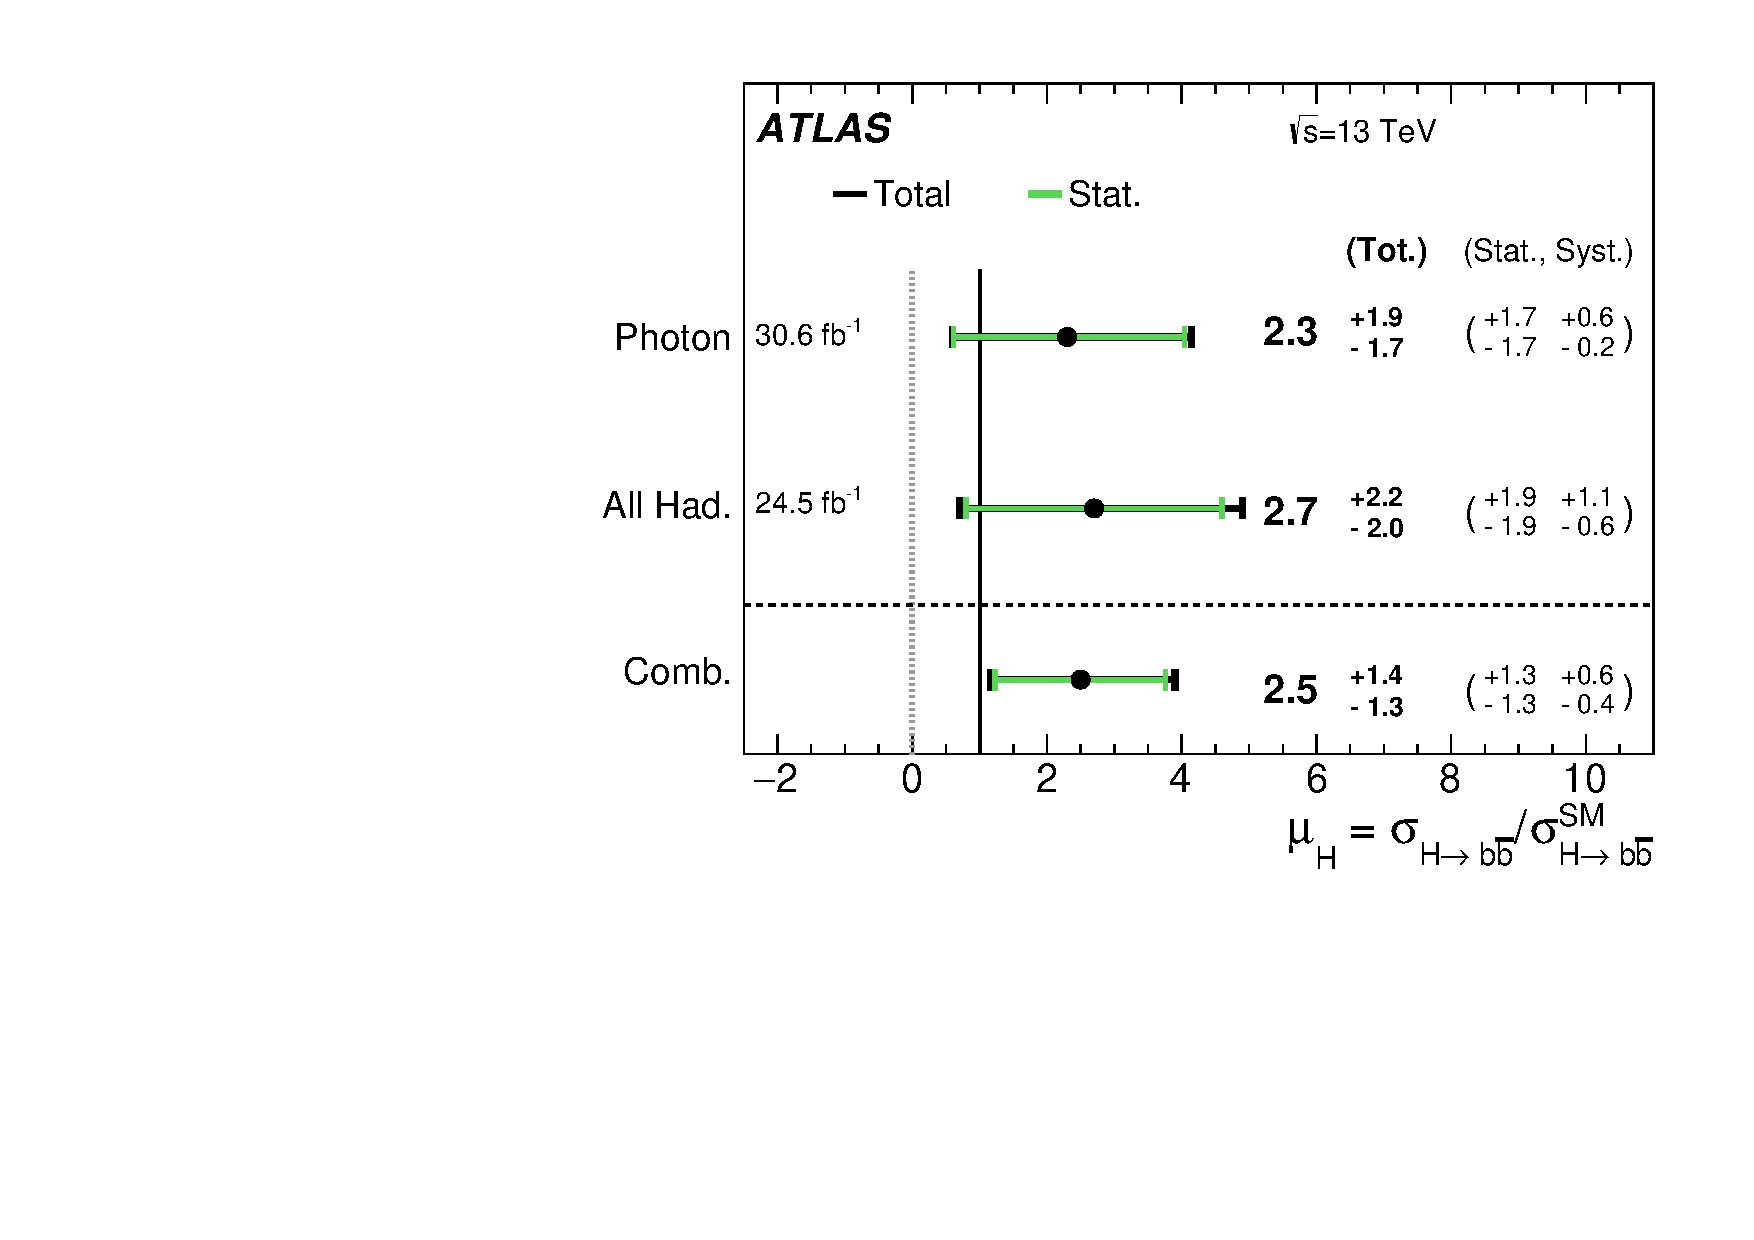
\includegraphics[width=0.49\textwidth]{figures/VBF/Plot_mu_summary_VBF.pdf}
  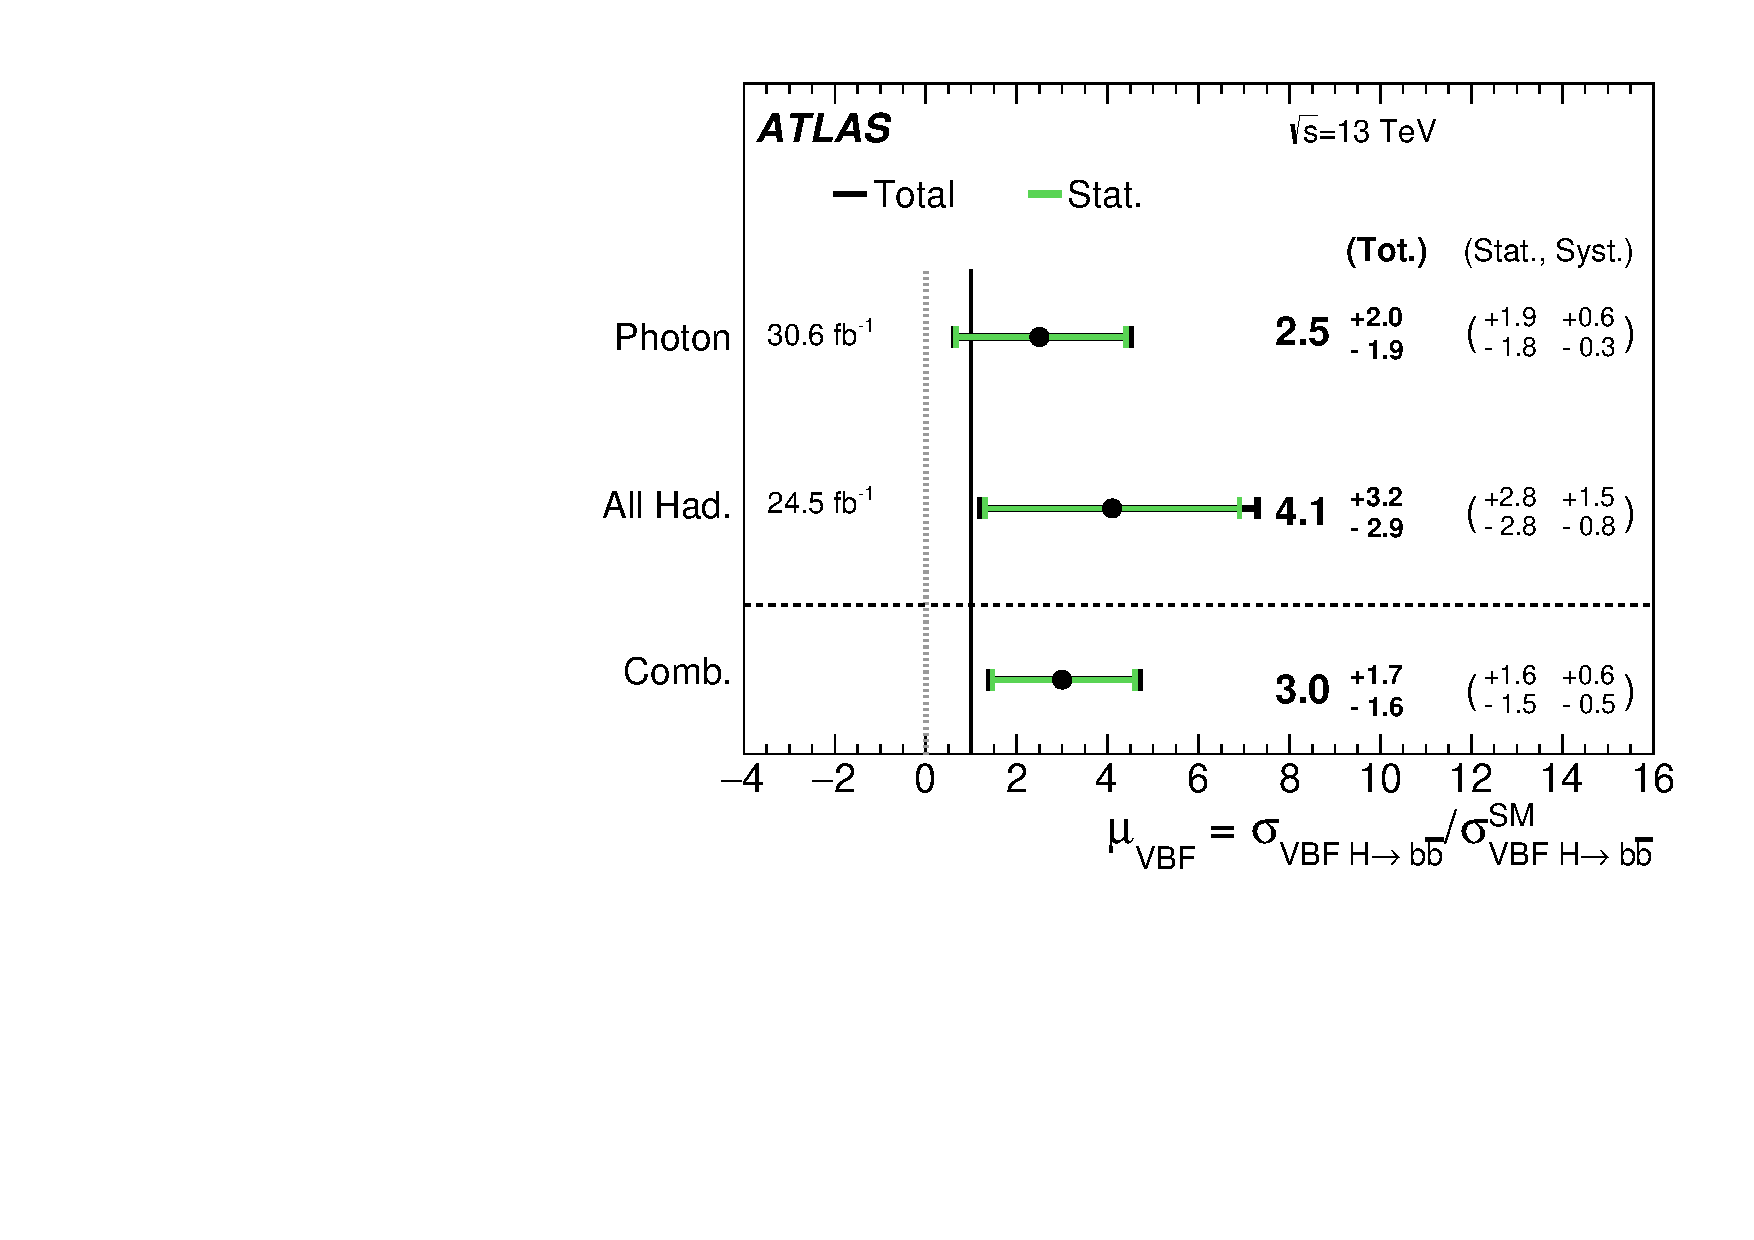
\includegraphics[width=0.49\textwidth]{figures/VBF/Plot_mu_summary_VBFonly.pdf}

\caption{Summary of the extraction of $\mu_{H}$(left) and $\mu_{VBF}$(right) for  \textit{all-hadronic}, \textit{photon} and combination fits.}
  \label{fig:vbf-summary}
\end{figure}



%\begin{figure}[htbp]
%  \centering
% 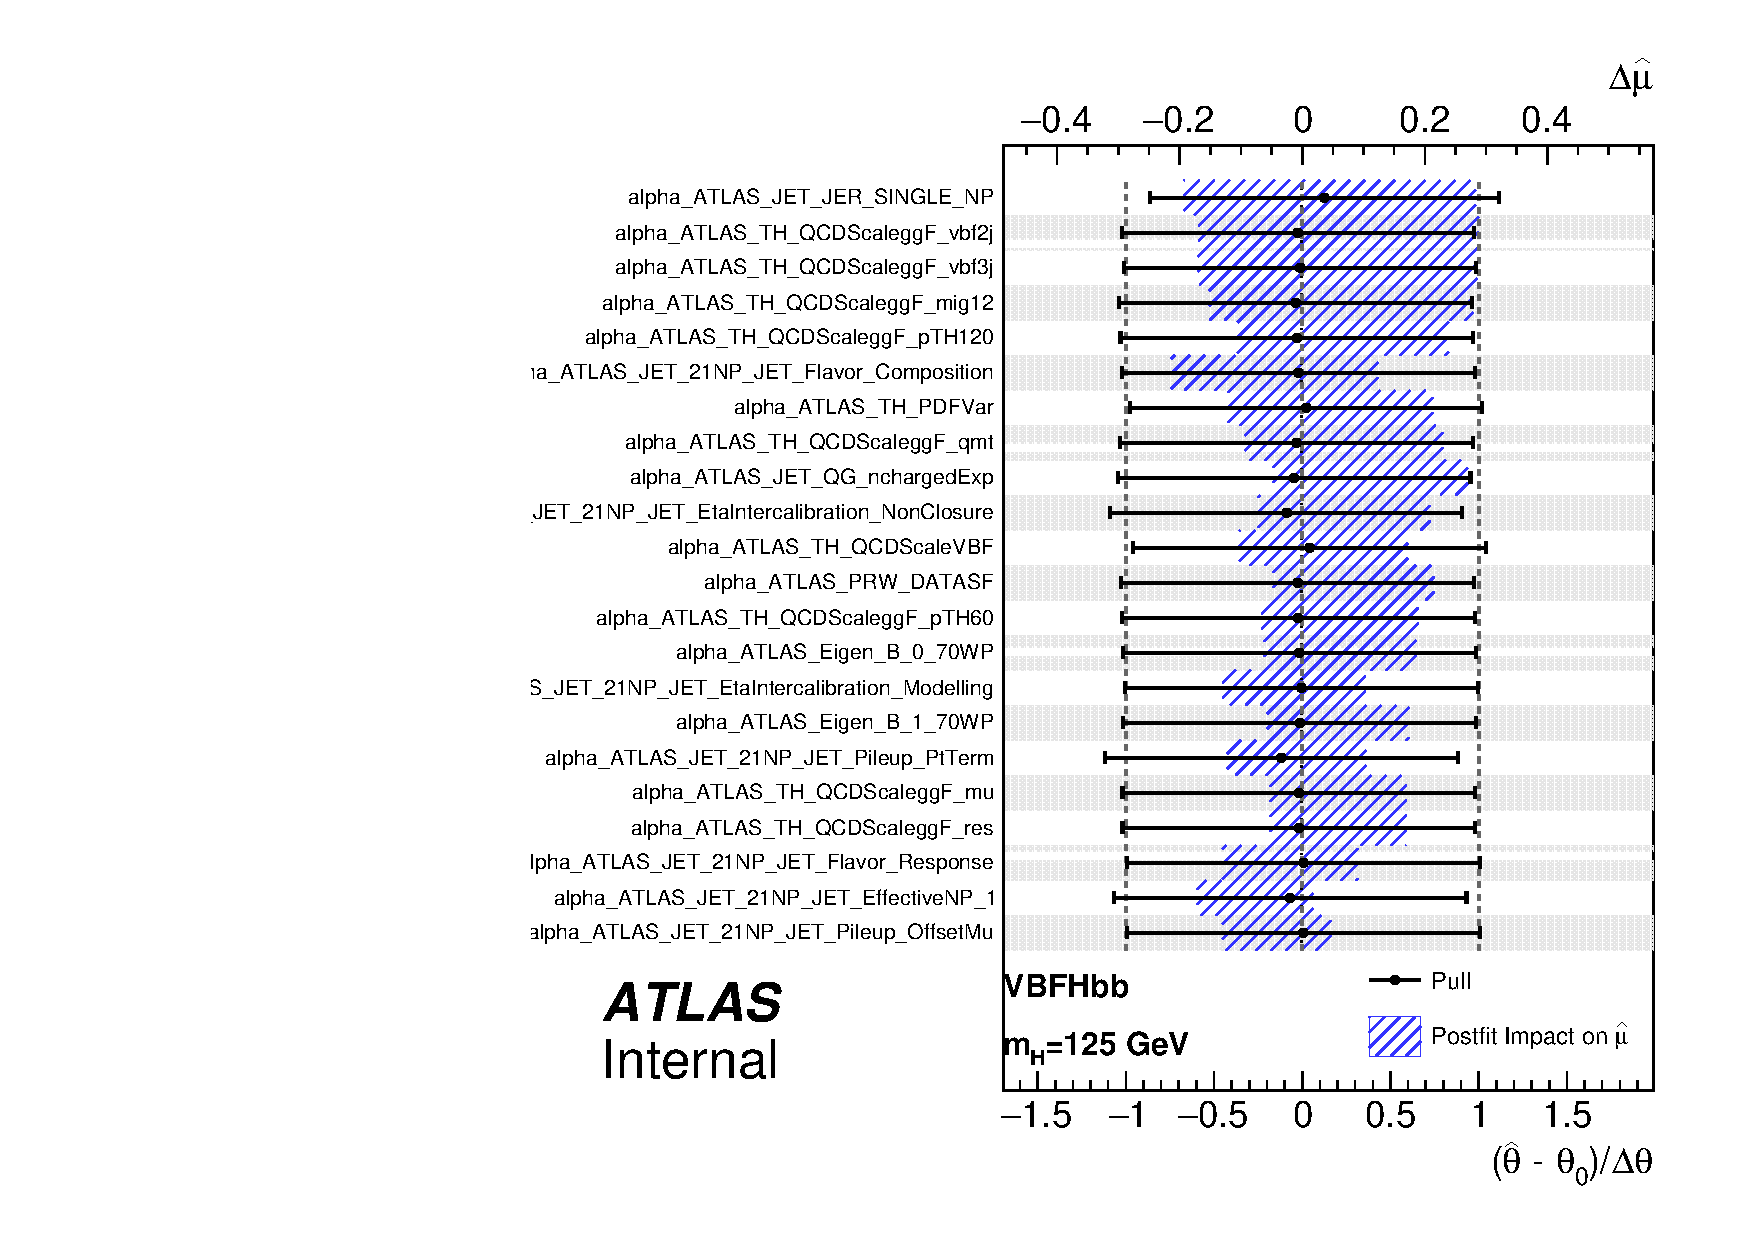
\includegraphics[width=0.8\textwidth]{figures/VBF/VBFHbb_pulls_125.pdf}
% \caption{Nuisance parameter post-fit impact and pulls are plotted for the data fit. Only the constrained NPs are shown. The uncertainties follow the naming defined in Table. \ref{tab:systnames}.}
%  \label{fig:vbf-higgsfitpull}
%\end{figure}

Regarding the treatment of uncertainties, both the inclusive and photon analyses apply systematics trimming. The inclusive analyses ignore nuisance parameters with yield impact $<0.5\%$ while the photon analysis ignore systematics with yield impact $<1\%$. Some NPs, for instance the third effective NP of jet energy scale may pass the systematics trimming cut of one analysis but not the other and therefore only show up in the combination fit for one analysis. 

Same set of nuisance parameters of detector related uncertainties including jet energy scale/resolution, luminosity, pile-up reweighting and q/g tagging is used by both analyses and hence treated as correlated.  $b$-tagging related uncertainties are an exception because the operating points are different between the two analyses. The inclusive analysis uses 70\% and 85\% WPs for \twocentral and \fourcentral channels respectively and the VBF$+\gamma$ analysis uses the 77\% WP. We experimented correlating NPs of the $b$-tagging uncertainties with highest impact, e.g. alpha\_FT\_EFF\_Eigen\_B\_0 of different WPs, across the two analyses and observed negligible change in the final result. Therefore the $b$-tagging NPs are left to be un-correlated.

Common terms of theoretical uncertainties including QCD scale of VBF process, parton shower and variation of $ttH$ yield are also correlated as the underlying variations are derived with same approaches. Background systematics such as non-resonant background normalization/parameterization, Z normalization and spurious signals are specific to each analysis and are not correlated.

The combination fit pull for $\mu_H$ is shown in Fig.\ref{fig:vbf-higgsfitpull_combination}. The combination fit pull for $\mu_{VBF}$ is shown in Fig.\ref{fig:vbf-vbffitpull_combination}. None of the systematics nuisance parameters are pulled significantly from their central values. One event display for the SRI of the \twocentral channel, the most sensitive BDT region, is shown in Fig.\ref{fig:vbf-evtdisplay}.


%%% no longer needed as VBF inclusive breaks down the QCD scale for VBF and ggF separately:  The inclusive and VBF$+\gamma$ analyses have some overlaps in the treatment of the QCD scale uncertainty although do not use exactly the same procedure therefore, by default, it is treated as uncorrelated.  The VBF$+\gamma$ analysis generates samples at truth level with changes by factors of two in the QCD scale and then does a truth-level calculation of the impact on the acceptance and normalization.  This analysis uses weights generated according to the \textit{WG1 scheme} (see Section~\ref{sec:vbf-syst_model}). Since it is a large systematic uncertainty for both analyses, we also try to correlate this particular nuisance parameter. The combined fit correlating the QCD scale uncertainty yields $\mu_H = 2.40^{+1.37}_{-1.32}$, which has a negligible difference with respect to the uncorrelated treatment. Hence we eventually adopt the result treating QCD scale as un-correlated as it is a more conservative approach. 


\begin{figure}[htbp]
  \centering
 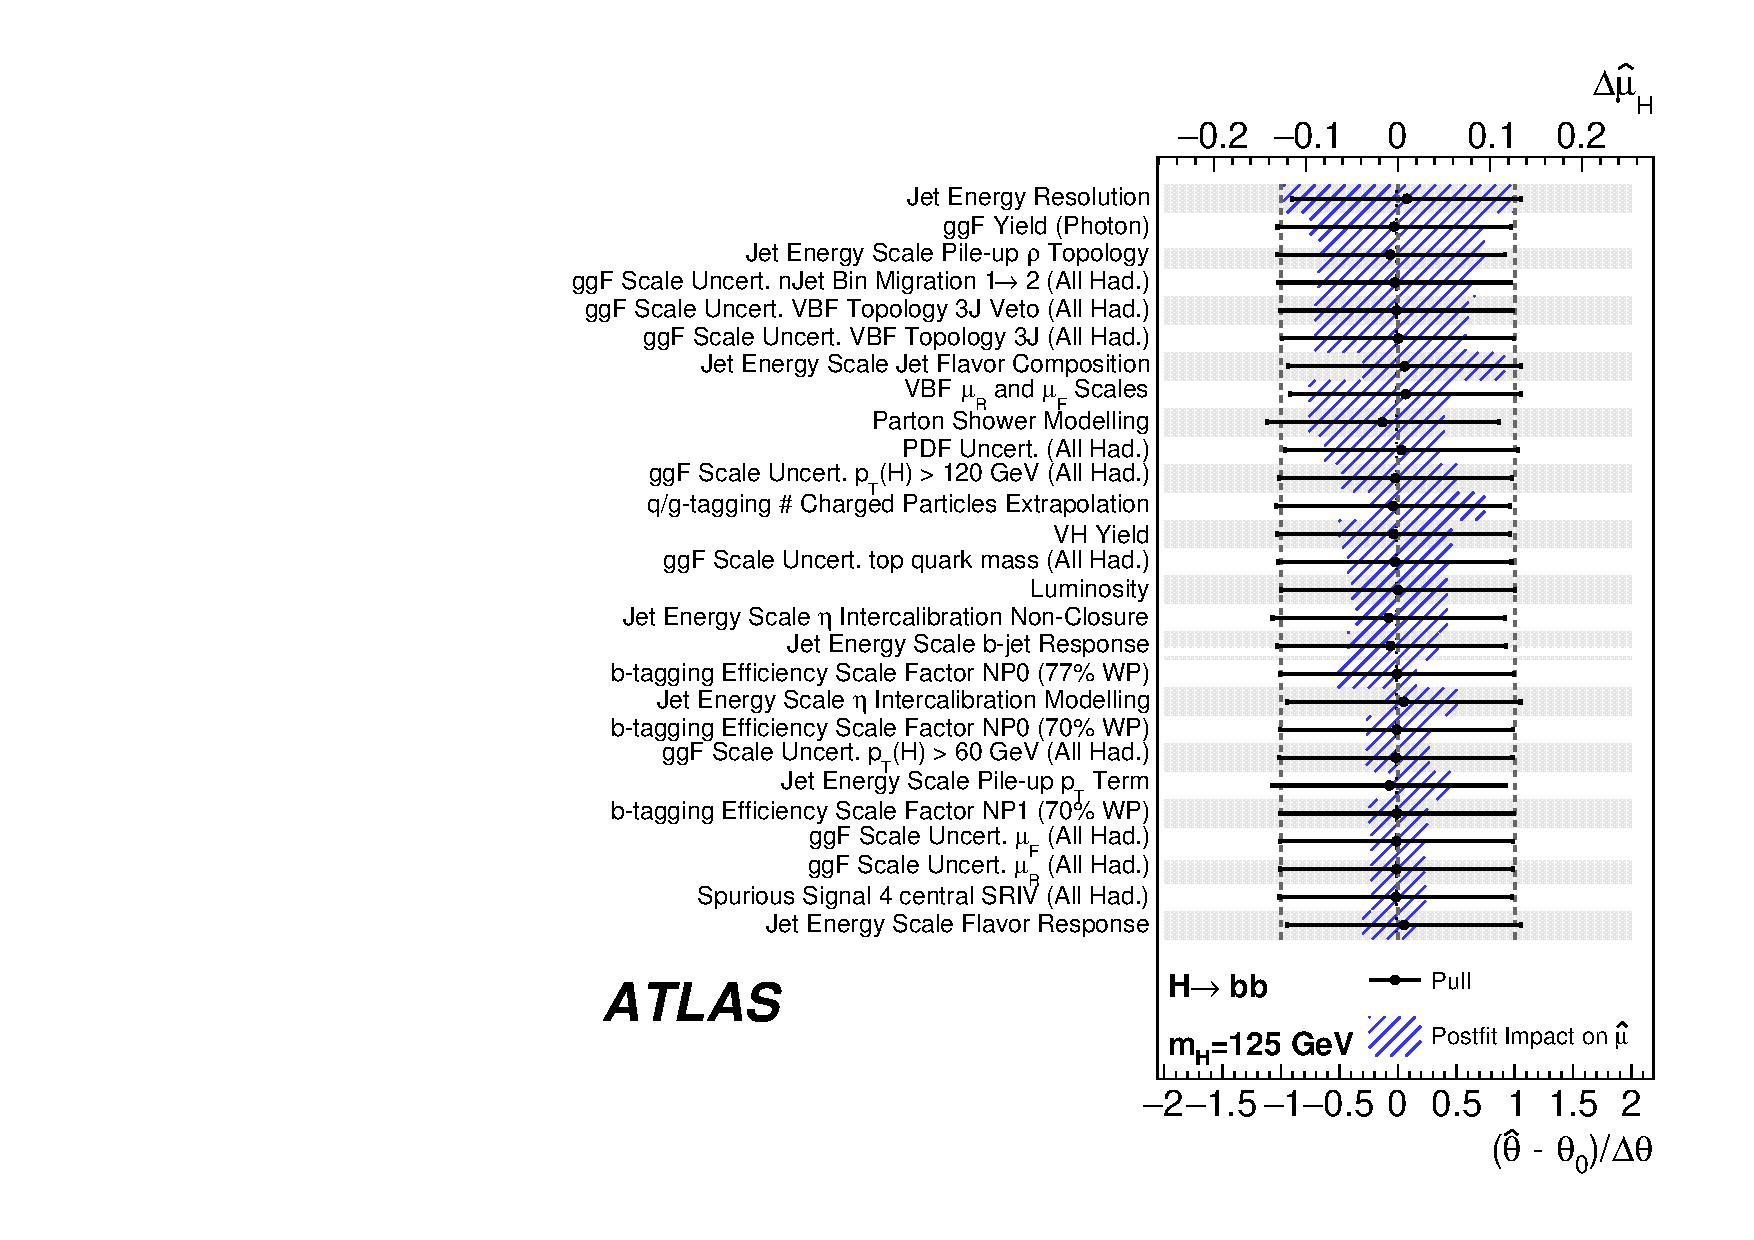
\includegraphics[width=0.8\textwidth]{figures/VBF/VBFHbb_Combined_pulls_125.pdf}
\caption{Data fit pulls for nuisance parameters with a post-fit impact $> 2$ \% for $\mu_H$ combining VBF inclusive and VBF$+\gamma$ analyses.}
  \label{fig:vbf-higgsfitpull_combination}
\end{figure}

\begin{figure}[htbp]
  \centering
 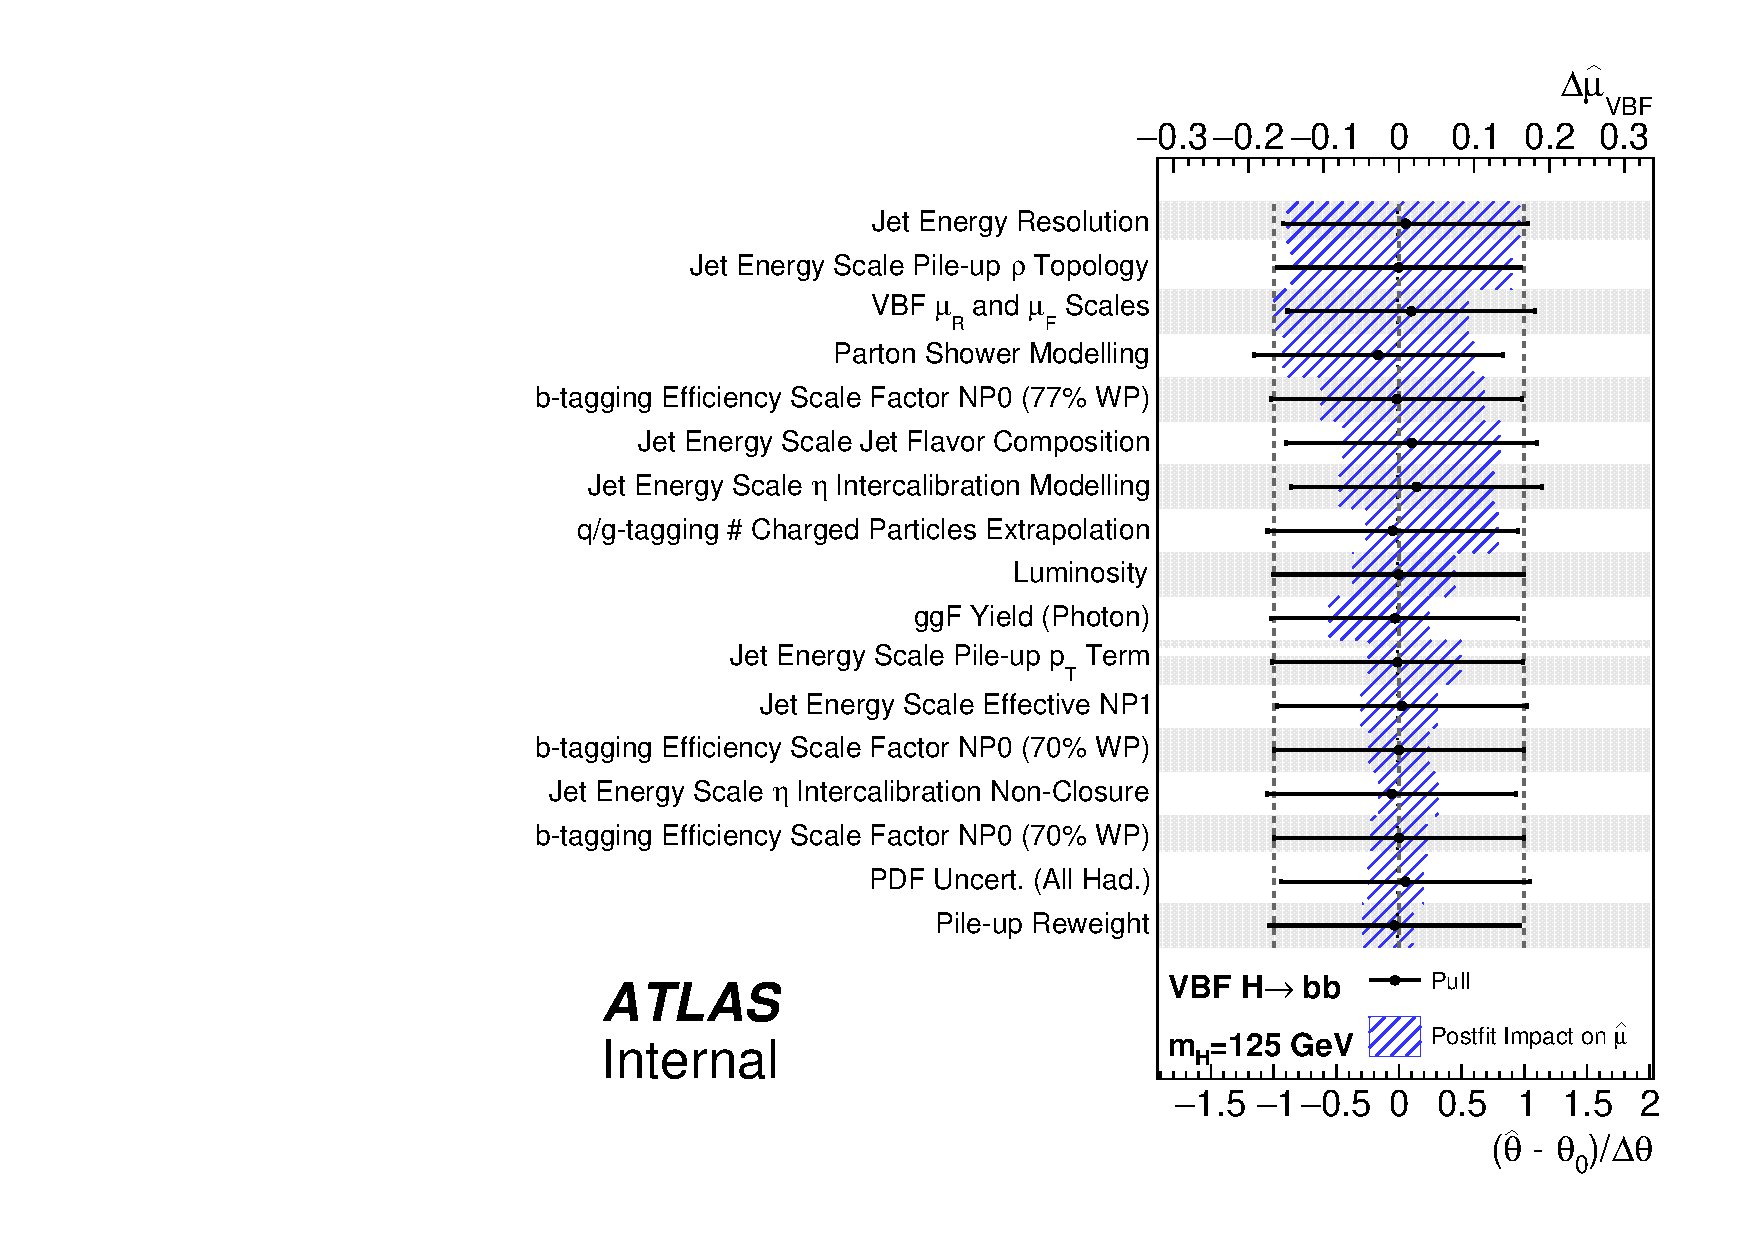
\includegraphics[width=0.8\textwidth]{figures/VBF/VBFHbb_Combined_vbfonly_pulls_125.pdf}
\caption{Data fit pulls for nuisance parameters with a post-fit impact $> 2$ \% for $\mu_{VBF}$ combining VBF inclusive and VBF$+\gamma$ analyses.}
  \label{fig:vbf-vbffitpull_combination}
\end{figure}


\begin{figure}[htbp]
  \centering
 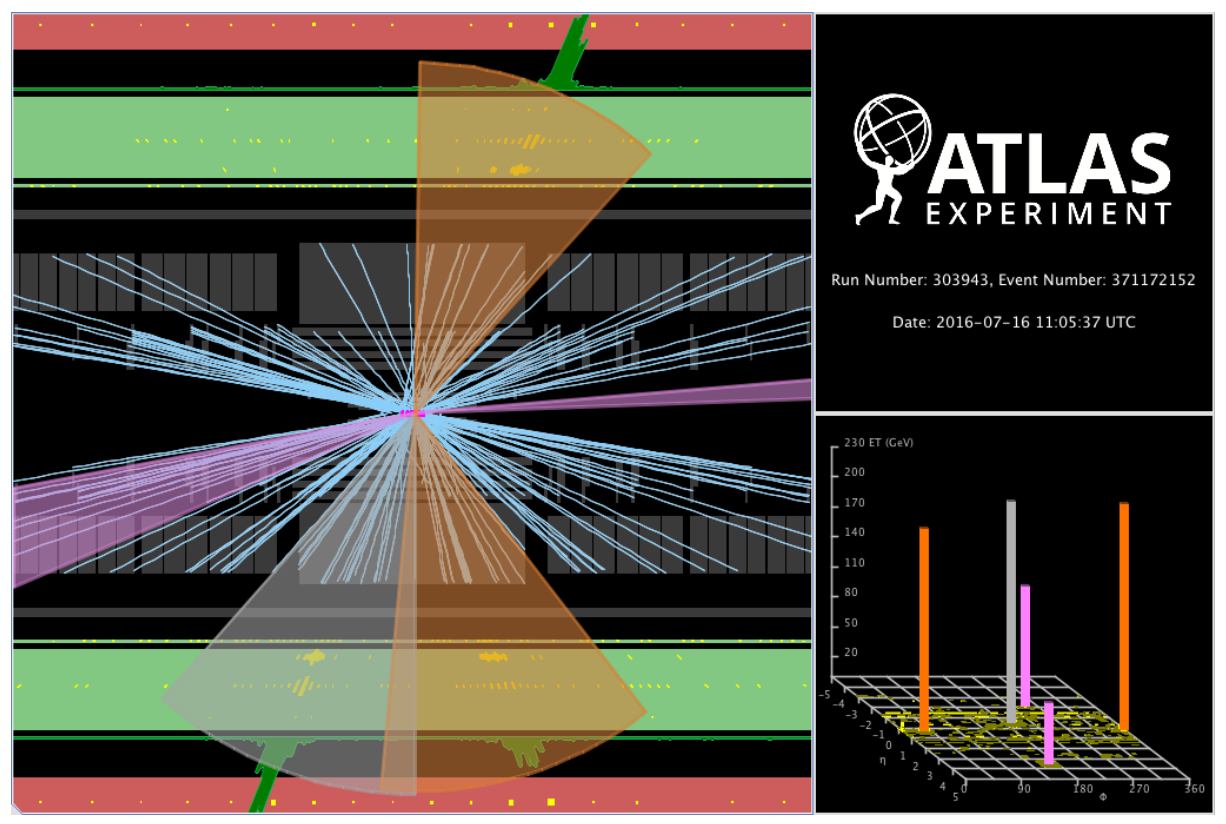
\includegraphics[width=0.8\textwidth]{figures/VBF/EvtDisplay2cen}
\caption{Event display of a \twocentral candidate event in SR I of the with \Mbb = 147 GeV. The cones representing the jets are colored magenta for the forward jets and orange for the b-tagged jets. The transverse momenta of the leading forward jet and sub-leading forward jet are 130.5 GeV and 82.0 GeV respectively. The pseudorapidity of the leading forward jet and sub-leading forward jet are -2.0 and 3.6 respectively}
  \label{fig:vbf-evtdisplay}
\end{figure}



%-------------------------------------------------------------------------------

\FloatBarrier

%-------------------------------------------------------------------------------
\section{Conclusion}
\label{sec:conclusion}
%-------------------------------------------------------------------------------

This paper presents a measurement of various properties of $g\rightarrow b\bar{b}$ at high $p_\text{T}$ and low $\Delta R(b,b)$ from 33 fb$^{-1}$ of $\sqrt{s}=13$ TeV $pp$ collisions recorded by the ATLAS detector.  A flavor-fraction fit is used to remove contributions from processes other than $g\rightarrow b\bar{b}$.  The fitted fractions significantly disagree with the pre-fit \PYTHIA predictions and suggest that further studies could improve the modeling of analyses sensitive to these fractions.  The measured properties are unfolded to correct for the detector acceptance and resolution for direct comparison to particle-level models.  Comparisons are made at particle level between the distributions and various models of jet formation. Simulations from the \SHERPA event generator generally provide a better model than \PYTHIA, especially for the $\Delta\mathrm{\theta}_\text{ppg,gbb}$ observable which is sensitive to the modeling of the gluon polarization. The particle-level spectra are publicly available~\cite{hepdata} for further interpretation and can be used to validate QCD MC predictions and tune their models' free parameters.

%-------------------------------------------------------------------------------
\section*{Acknowledgements}
%-------------------------------------------------------------------------------

% Acknowledgements for papers with collision data
% Version 14-Feb-2018

% Standard acknowledgements start here
%----------------------------------------------
We thank CERN for the very successful operation of the LHC, as well as the
support staff from our institutions without whom ATLAS could not be
operated efficiently.

We acknowledge the support of ANPCyT, Argentina; YerPhI, Armenia; ARC, Australia; BMWFW and FWF, Austria; ANAS, Azerbaijan; SSTC, Belarus; CNPq and FAPESP, Brazil; NSERC, NRC and CFI, Canada; CERN; CONICYT, Chile; CAS, MOST and NSFC, China; COLCIENCIAS, Colombia; MSMT CR, MPO CR and VSC CR, Czech Republic; DNRF and DNSRC, Denmark; IN2P3-CNRS, CEA-DRF/IRFU, France; SRNSFG, Georgia; BMBF, HGF, and MPG, Germany; GSRT, Greece; RGC, Hong Kong SAR, China; ISF, I-CORE and Benoziyo Center, Israel; INFN, Italy; MEXT and JSPS, Japan; CNRST, Morocco; NWO, Netherlands; RCN, Norway; MNiSW and NCN, Poland; FCT, Portugal; MNE/IFA, Romania; MES of Russia and NRC KI, Russian Federation; JINR; MESTD, Serbia; MSSR, Slovakia; ARRS and MIZ\v{S}, Slovenia; DST/NRF, South Africa; MINECO, Spain; SRC and Wallenberg Foundation, Sweden; SERI, SNSF and Cantons of Bern and Geneva, Switzerland; MOST, Taiwan; TAEK, Turkey; STFC, United Kingdom; DOE and NSF, United States of America. In addition, individual groups and members have received support from BCKDF, the Canada Council, CANARIE, CRC, Compute Canada, FQRNT, and the Ontario Innovation Trust, Canada; EPLANET, ERC, ERDF, FP7, Horizon 2020 and Marie Sk{\l}odowska-Curie Actions, European Union; Investissements d'Avenir Labex and Idex, ANR, R{\'e}gion Auvergne and Fondation Partager le Savoir, France; DFG and AvH Foundation, Germany; Herakleitos, Thales and Aristeia programmes co-financed by EU-ESF and the Greek NSRF; BSF, GIF and Minerva, Israel; BRF, Norway; CERCA Programme Generalitat de Catalunya, Generalitat Valenciana, Spain; the Royal Society and Leverhulme Trust, United Kingdom.

The crucial computing support from all WLCG partners is acknowledged gratefully, in particular from CERN, the ATLAS Tier-1 facilities at TRIUMF (Canada), NDGF (Denmark, Norway, Sweden), CC-IN2P3 (France), KIT/GridKA (Germany), INFN-CNAF (Italy), NL-T1 (Netherlands), PIC (Spain), ASGC (Taiwan), RAL (UK) and BNL (USA), the Tier-2 facilities worldwide and large non-WLCG resource providers. Major contributors of computing resources are listed in Ref.~\cite{ATL-GEN-PUB-2016-002}.
%----------------------------------------------



%-------------------------------------------------------------------------------
\clearpage
%\appendix
%\part*{Appendix}
%\addcontentsline{toc}{part}{Appendix}
%-------------------------------------------------------------------------------

%In a paper, an appendix is used for technical details that would otherwise disturb the flow of the paper.
%Such an appendix should be printed before the Bibliography.

%-------------------------------------------------------------------------------
% If you use biblatex and either biber or bibtex to process the bibliography
% just say \printbibliography here
\printbibliography
% If you want to use the traditional BibTeX you need to use the syntax below.
%\bibliographystyle{bib/bst/atlasBibStyleWoTitle}
%\bibliography{atlas-document,bib/ATLAS,bib/CMS,bib/ConfNotes,bib/PubNotes}
%-------------------------------------------------------------------------------

%-------------------------------------------------------------------------------
% Auxiliary material - comment out the following line if you do not have any
\include{atlas-document-auxmat}
%-------------------------------------------------------------------------------

\clearpage

\begin{figure}[htbp]
  \centering
 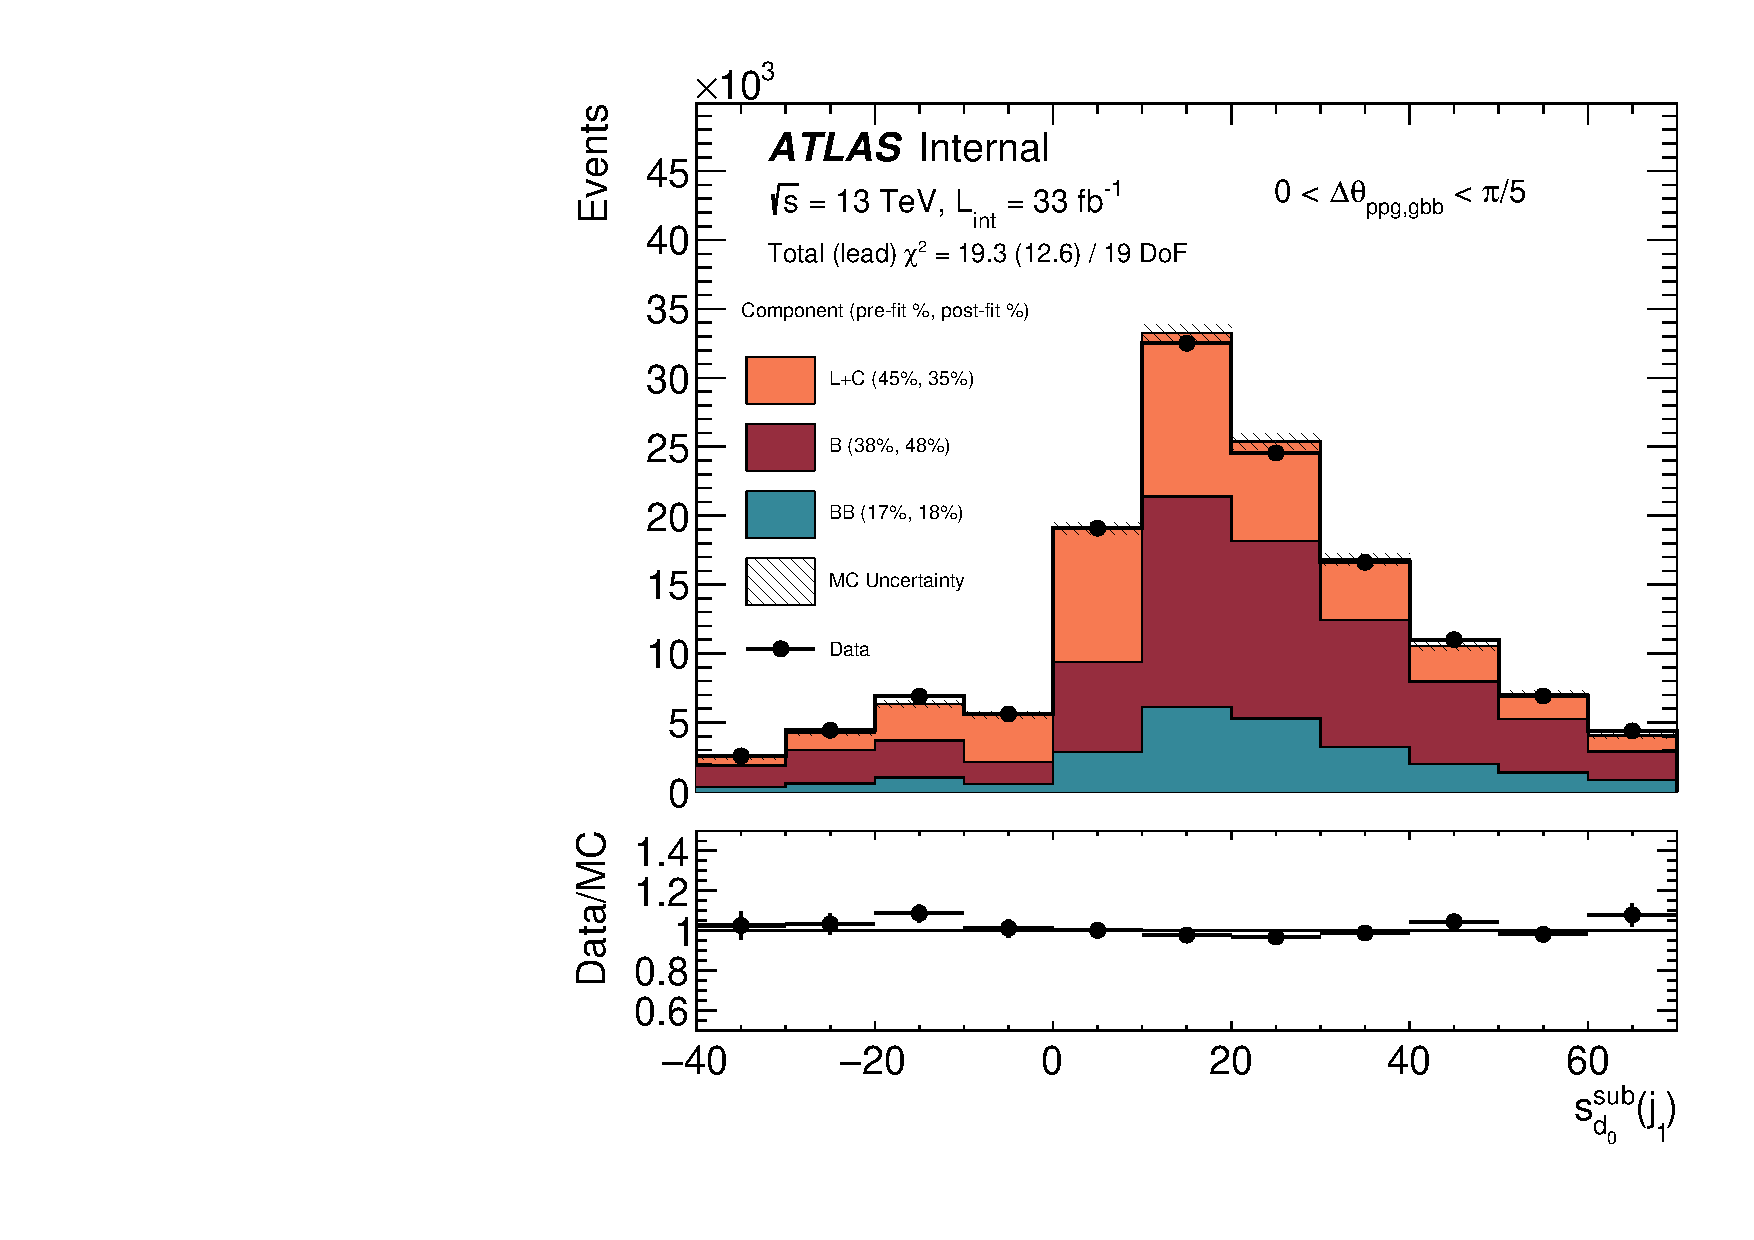
\includegraphics[width=0.48\textwidth]{figures/Canv_Fit_dphi_LpT_INF_SpT_INF_coarse_x}
 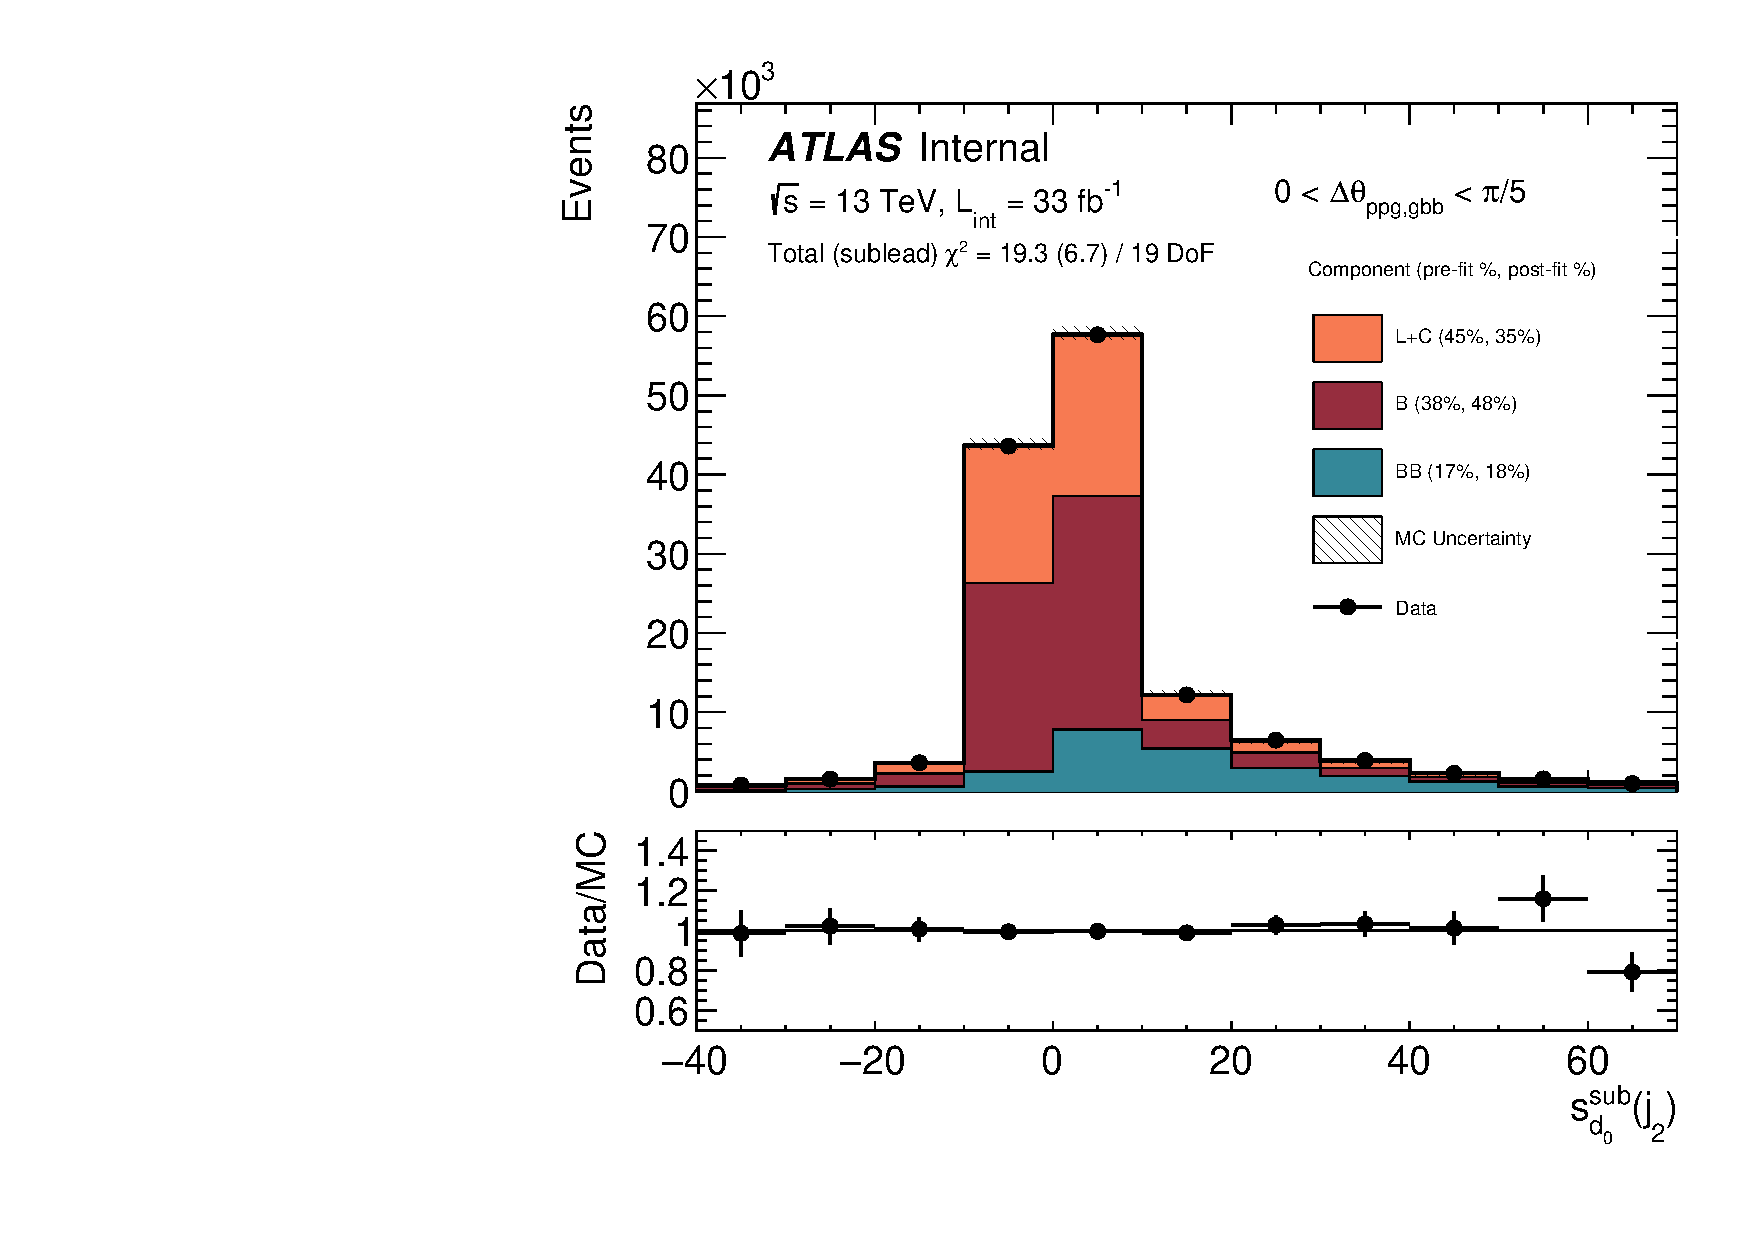
\includegraphics[width=0.48\textwidth]{figures/Canv_Fit_b0_25_dphi_0_3_LpT_INF_SpT_INF_coarse_y}\\
\caption{The distribution of $\subsdzero$ in simulation, post-fit, for the higher $p_\text{T}$ track-jet (left) and for the lower $p_\text{T}$ track-jet (right) in the bin $0<\Delta\mathrm{\theta}_\text{ppg,gbb}<\pi/5$. The three components are the signal double-$b$ (`BB'), the background single $b$ (`B'), and the background non-$b$ components (`L+C').  Percentages reported in the legend indicate the pre- and post-fit fraction of each component.  Only data and MC statistical uncertainties are shown.}
  \label{fig:fits2}
\end{figure}

\begin{figure}[htbp]
  \centering
 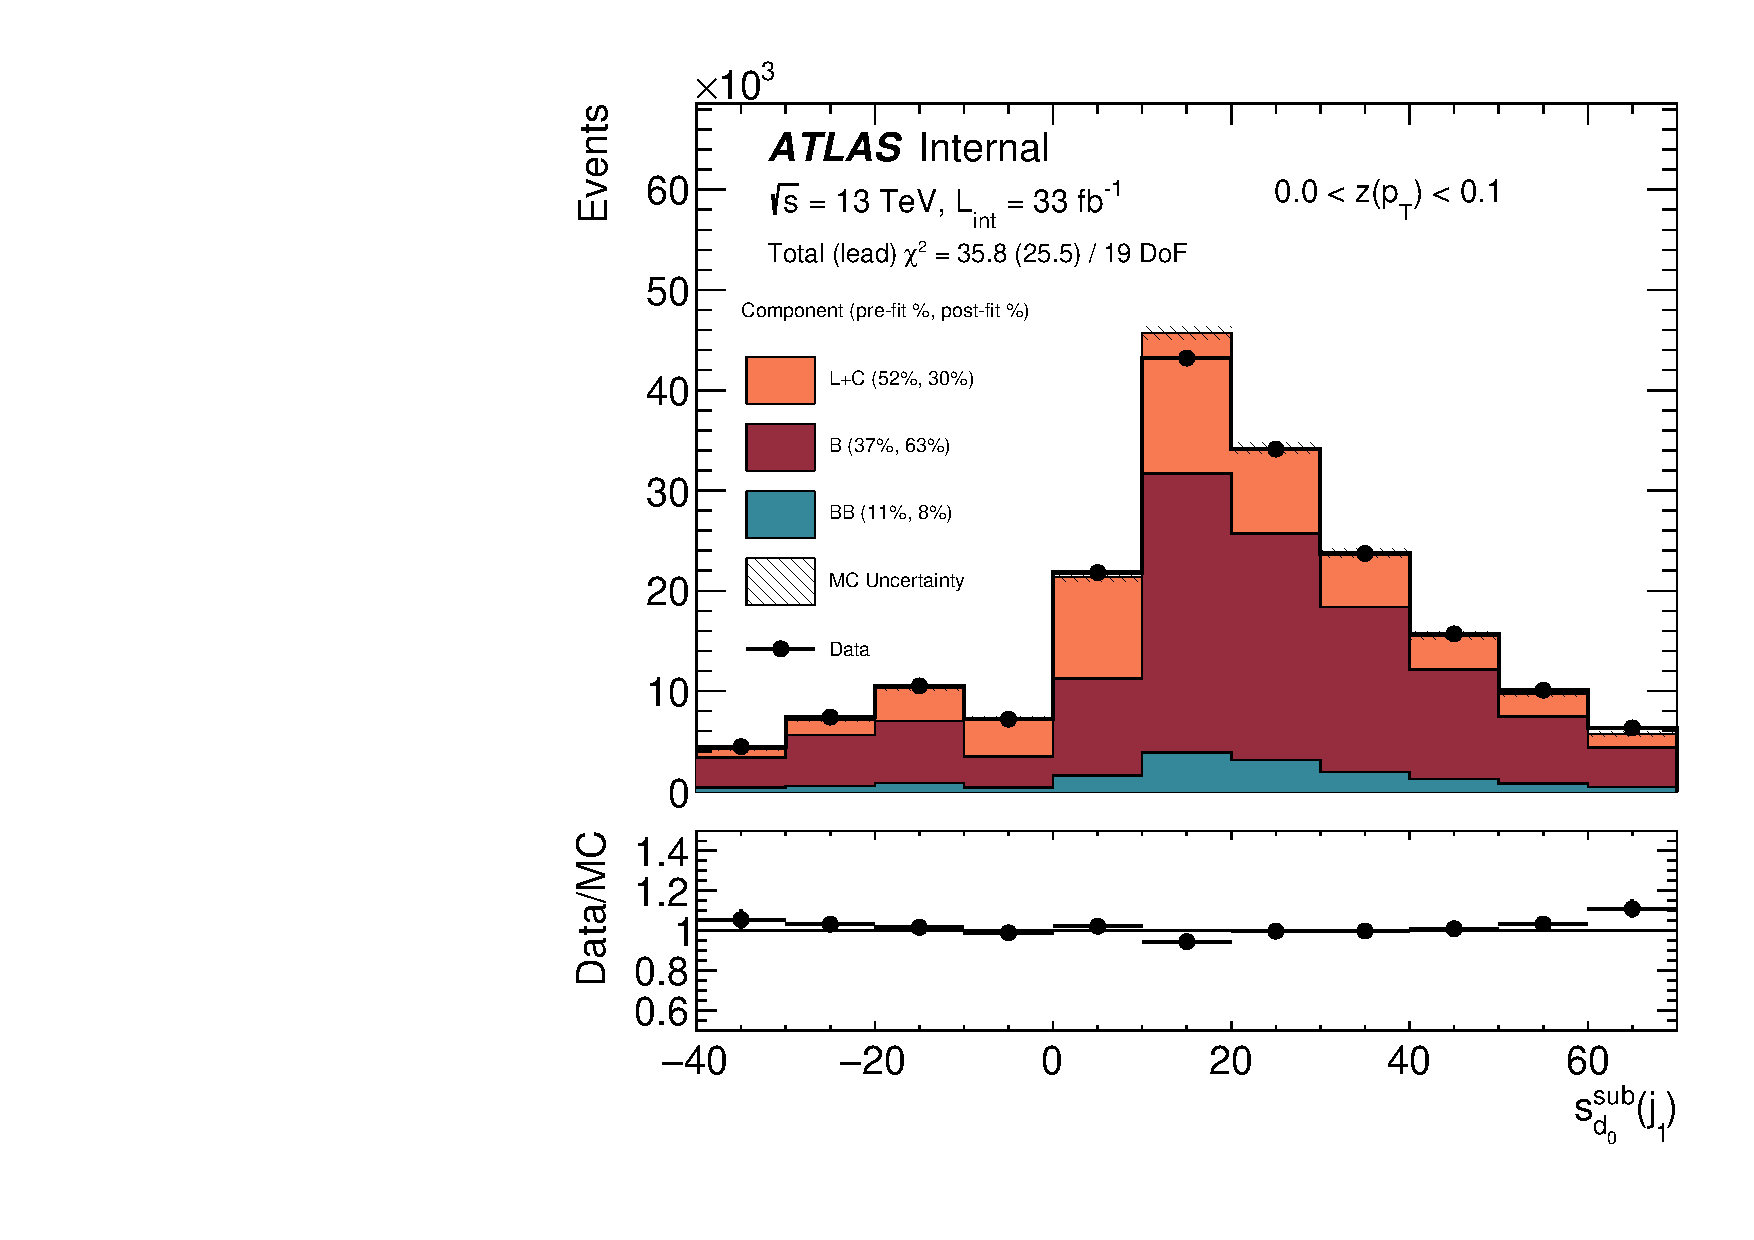
\includegraphics[width=0.48\textwidth]{figures/Canv_Fit_zpt_LpT_INF_SpT_INF_coarse_x}
 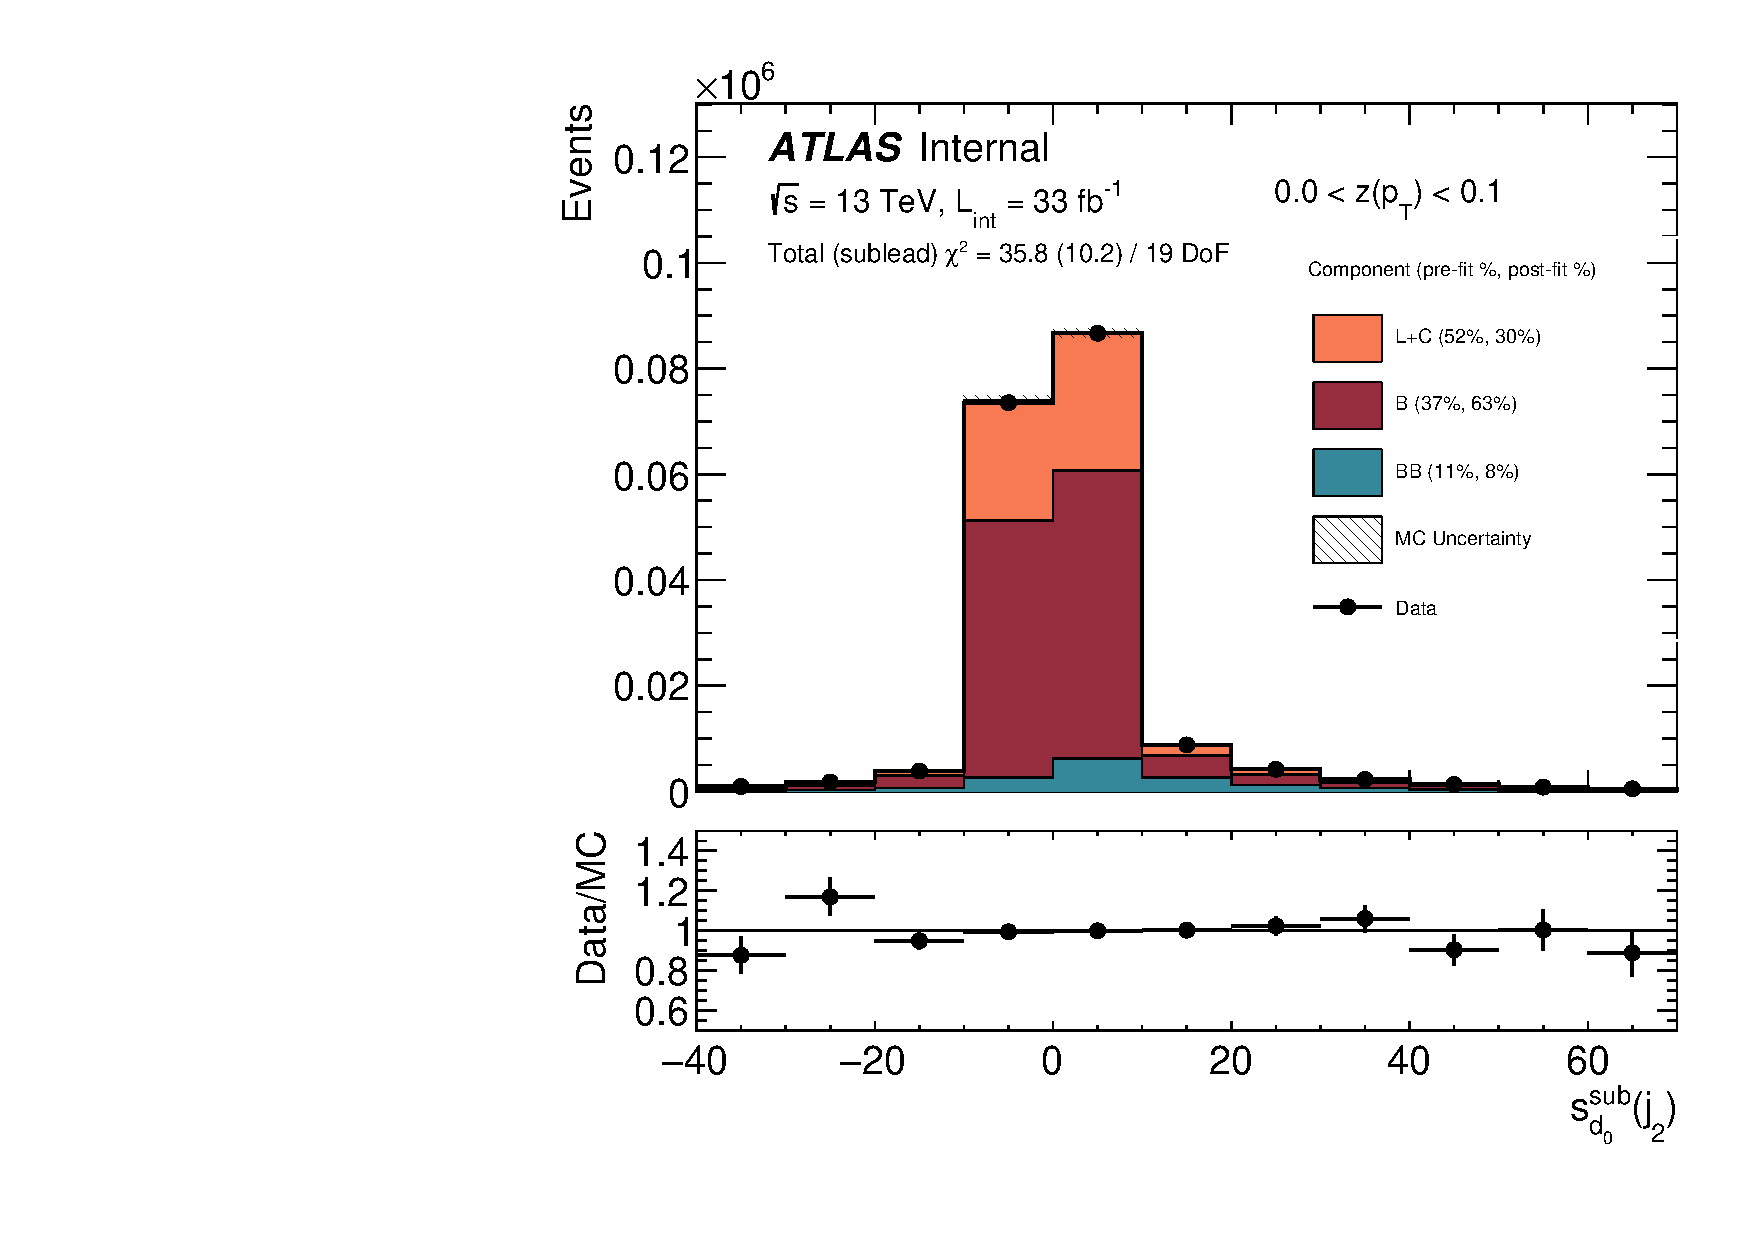
\includegraphics[width=0.48\textwidth]{figures/Canv_Fit_b0_25_zpt_0_3_LpT_INF_SpT_INF_coarse_y.pdf}\\
\caption{The distribution of $\subsdzero$ in simulation, post-fit, for the higher $p_\text{T}$ track-jet (left) and for the lower $p_\text{T}$ track-jet (right) in the bin $0.0<z(p_\text{T})<0.1$. The three components are the signal double-$b$ (`BB'), the background single $b$ (`B'), and the background non-$b$ components (`L+C').  Percentages reported in the legend indicate the pre- and post-fit fraction of each component.  Only data and MC statistical uncertainties are shown.}
  \label{fig:fits3}
\end{figure}

\begin{figure}[htbp]
  \centering
 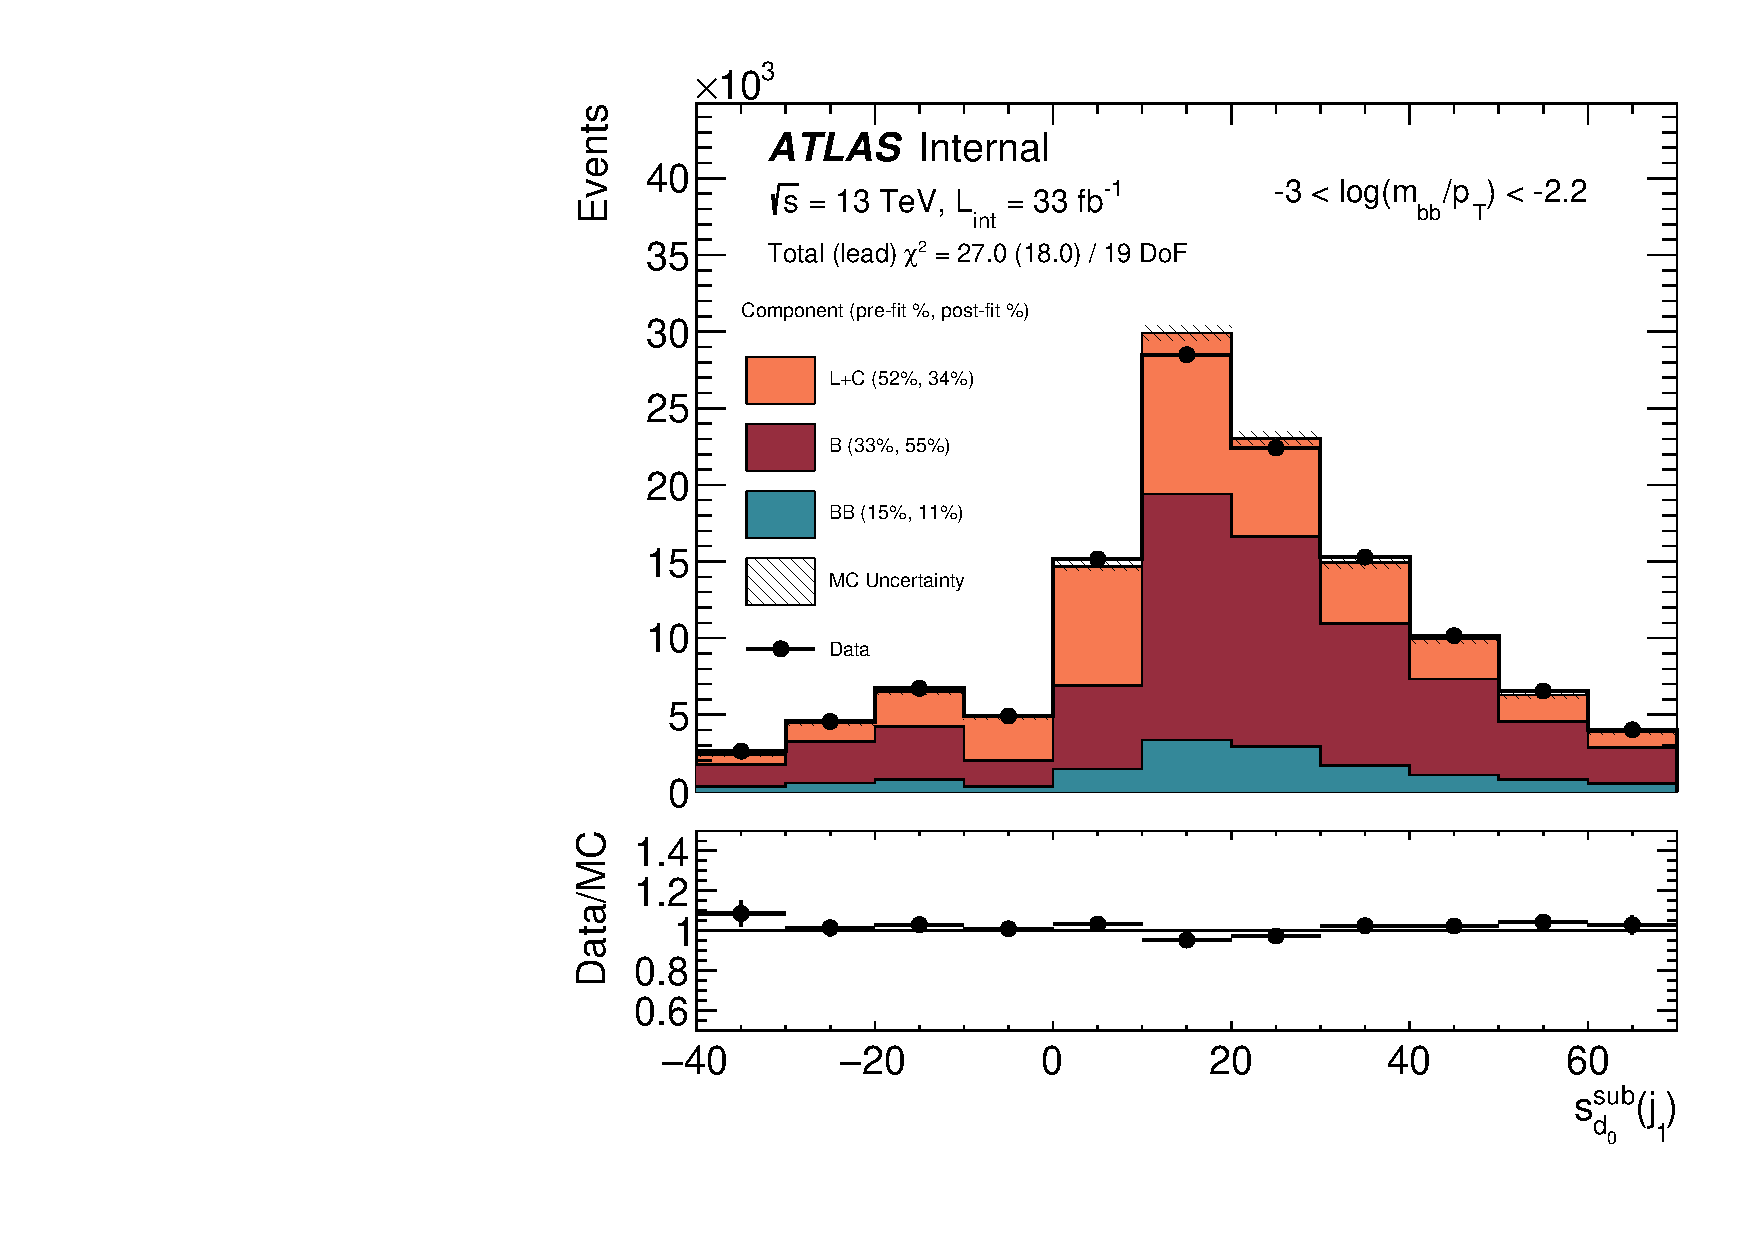
\includegraphics[width=0.48\textwidth]{figures/Canv_Fit_M_LpT_INF_SpT_INF_coarse_x}
 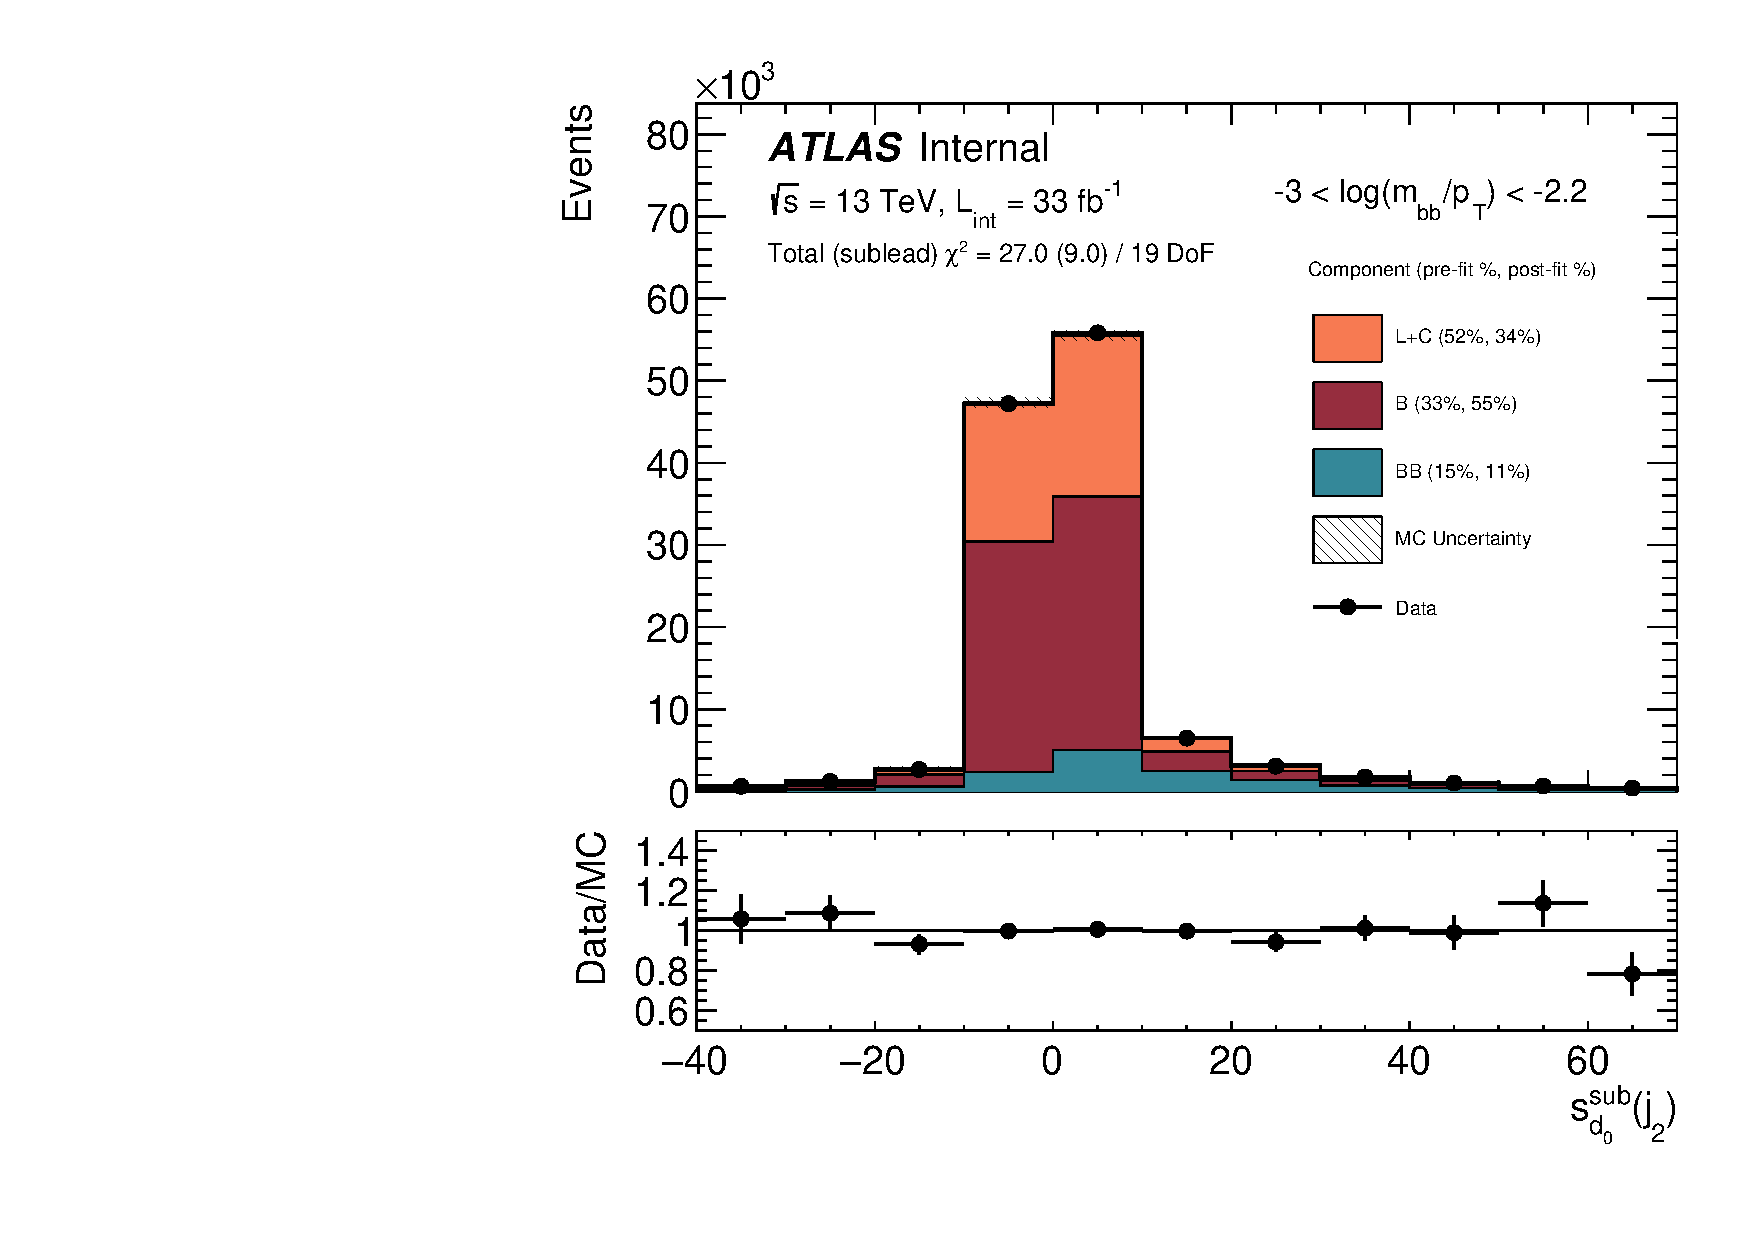
\includegraphics[width=0.48\textwidth]{figures/Canv_Fit_b0_25_M_0_3_LpT_INF_SpT_INF_coarse_y}\\
\caption{The distribution of $\subsdzero$ in simulation, post-fit, for the higher $p_\text{T}$ track-jet (left) and for the lower $p_\text{T}$ track-jet (right) in the bin $-3.0<\log(m/p_\text{T})<-2.2$. The three components are the signal double-$b$ (`BB'), the background single $b$ (`B'), and the background non-$b$ components (`L+C').  Percentages reported in the legend indicate the pre- and post-fit fraction of each component.  Only data and MC statistical uncertainties are shown.}
  \label{fig:fits4}
\end{figure}

%-------------------------------------------------------------------------------
% Extra tables etc. for HepData - comment in the following line if you have any
% \include{atlas-document-hepdata}
%-------------------------------------------------------------------------------

\end{document}
